% uWaterloo Thesis Template for LaTeX 
% Last Updated May 24, 2011 by Stephen Carr, IST Client Services
% FOR ASSISTANCE, please send mail to rt-IST-CSmathsci@ist.uwaterloo.ca

% Effective October 2006, the University of Waterloo 
% requires electronic thesis submission. See the uWaterloo thesis regulations at
% http://www.grad.uwaterloo.ca/Thesis_Regs/thesistofc.asp.

% DON'T FORGET TO ADD YOUR OWN NAME AND TITLE in the "hyperref" package
% configuration below. THIS INFORMATION GETS EMBEDDED IN THE PDF FINAL PDF DOCUMENT.
% You can view the information if you view Properties of the PDF document.

% Many faculties/departments also require one or more printed
% copies. This template attempts to satisfy both types of output. 
% It is based on the standard "book" document class which provides all necessary 
% sectioning structures and allows multi-part theses.

% DISCLAIMER
% To the best of our knowledge, this template satisfies the current uWaterloo requirements.
% However, it is your responsibility to assure that you have met all 
% requirements of the University and your particular department.
% Many thanks to the feedback from many graduates that assisted the development of this template.

% -----------------------------------------------------------------------

% By default, output is produced that is geared toward generating a PDF 
% version optimized for viewing on an electronic display, including 
% hyperlinks within the PDF.

% E.g. to process a thesis called "mythesis.tex" based on this template, run:

% pdflatex mythesis	-- first pass of the pdflatex processor
% bibtex mythesis	-- generates bibliography from .bib data file(s) 
% pdflatex mythesis	-- fixes cross-references, bibliographic references, etc
% pdflatex mythesis	-- fixes cross-references, bibliographic references, etc

% If you use the recommended LaTeX editor, Texmaker, you would open the mythesis.tex
% file, then click the pdflatex button. Then run BibTeX (under the Tools menu).
% Then click the pdflatex button two more times. If you have an index as well,
% you'll need to run MakeIndex from the Tools menu as well, before running pdflatex
% the last two times.

% N.B. The "pdftex" program allows graphics in the following formats to be
% included with the "\includegraphics" command: PNG, PDF, JPEG, TIFF
% Tip 1: Generate your figures and photos in the size you want them to appear
% in your thesis, rather than scaling them with \includegraphics options.
% Tip 2: Any drawings you do should be in scalable vector graphic formats:
% SVG, PNG, WMF, EPS and then converted to PNG or PDF, so they are scalable in
% the final PDF as well.
% Tip 3: Photographs should be cropped and compressed so as not to be too large.

% To create a PDF output that is optimized for double-sided printing: 
%
% 1) comment-out the \documentclass statement in the preamble below, and
% un-comment the second \documentclass line.
%
% 2) change the value assigned below to the boolean variable
% "PrintVersion" from "false" to "true".

% --------------------- Start of Document Preamble -----------------------

% Specify the document class, default style attributes, and page dimensions
% For hyperlinked PDF, suitable for viewing on a computer, use this:
\documentclass[letterpaper,12pt,titlepage,oneside,final]{book}

% For PDF, suitable for double-sided printing, change the PrintVersion variable below
% to "true" and use this \documentclass line instead of the one above:
%\documentclass[letterpaper,12pt,titlepage,openright,twoside,final]{book}

% Some LaTeX commands I define for my own nomenclature.
% If you have to, it's better to change nomenclature once here than in a 
% million places throughout your thesis!
\newcommand{\package}[1]{\textbf{#1}} % package names in bold text
\newcommand{\cmmd}[1]{\textbackslash\texttt{#1}} % command name in tt font 
\newcommand{\href}[1]{#1} % does nothing, but defines the command so the
% print-optimized version will ignore \href tags (redefined by hyperref pkg).
%\newcommand{\texorpdfstring}[2]{#1} % does nothing, but defines the command
% Anything defined here may be redefined by packages added below...

% This package allows if-then-else control structures.
\usepackage{ifthen}
\newboolean{PrintVersion}
\setboolean{PrintVersion}{false} 
% CHANGE THIS VALUE TO "true" as necessary, to improve printed results for hard copies
% by overriding some options of the hyperref package below.

%\usepackage{nomencl} % For a nomenclature (optional; available from ctan.org)
\usepackage{amsmath,amssymb,amstext} % Lots of math symbols and environments
\usepackage[pdftex]{graphicx} % For including graphics N.B. pdftex graphics driver 

\usepackage{mleftright}

\usepackage{algorithm}
\usepackage[noend]{algpseudocode}
\usepackage{amsmath}
\usepackage[section]{placeins}
\usepackage{color,soul}
\usepackage{caption}
\usepackage{subcaption}
\usepackage[overload]{empheq}
% Hyperlinks make it very easy to navigate an electronic document.
% In addition, this is where you should specify the thesis title
% and author as they appear in the properties of the PDF document.
% Use the "hyperref" package 
% N.B. HYPERREF MUST BE THE LAST PACKAGE LOADED; ADD ADDITIONAL PKGS ABOVE
\usepackage[pdftex,letterpaper=true,pagebackref=false]{hyperref} % with basic options
% N.B. pagebackref=true provides links back from the References to the body text. This can cause trouble for printing.
\hypersetup{
	plainpages=false,       % needed if Roman numbers in frontpages
	pdfpagelabels=true,     % adds page number as label in Acrobat's page count
	bookmarks=true,         % show bookmarks bar?
	unicode=false,          % non-Latin characters in Acrobat’s bookmarks
	pdftoolbar=true,        % show Acrobat’s toolbar?
	pdfmenubar=true,        % show Acrobat’s menu?
	pdffitwindow=false,     % window fit to page when opened
	pdfstartview={FitH},    % fits the width of the page to the window
	pdftitle={uWaterloo\ LaTeX\ Thesis\ Template},    % title: CHANGE THIS TEXT!
	%    pdfauthor={Author},    % author: CHANGE THIS TEXT! and uncomment this line
	%    pdfsubject={Subject},  % subject: CHANGE THIS TEXT! and uncomment this line
	%    pdfkeywords={keyword1} {key2} {key3}, % list of keywords, and uncomment this line if desired
	pdfnewwindow=true,      % links in new window
	colorlinks=true,        % false: boxed links; true: colored links
	linkcolor=blue,         % color of internal links
	citecolor=green,        % color of links to bibliography
	filecolor=magenta,      % color of file links
	urlcolor=cyan           % color of external links
}
\ifthenelse{\boolean{PrintVersion}}{   % for improved print quality, change some hyperref options
	\hypersetup{	% override some previously defined hyperref options
		%    colorlinks,%
		citecolor=black,%
		filecolor=black,%
		linkcolor=black,%
		urlcolor=black}
}{} % end of ifthenelse (no else)

% Setting up the page margins...
% uWaterloo thesis requirements specify a minimum of 1 inch (72pt) margin at the
% top, bottom, and outside page edges and a 1.125 in. (81pt) gutter
% margin (on binding side). While this is not an issue for electronic
% viewing, a PDF may be printed, and so we have the same page layout for
% both printed and electronic versions, we leave the gutter margin in.
% Set margins to minimum permitted by uWaterloo thesis regulations:
\setlength{\marginparwidth}{0pt} % width of margin notes
% N.B. If margin notes are used, you must adjust \textwidth, \marginparwidth
% and \marginparsep so that the space left between the margin notes and page
% edge is less than 15 mm (0.6 in.)
\setlength{\marginparsep}{0pt} % width of space between body text and margin notes
\setlength{\evensidemargin}{0.125in} % Adds 1/8 in. to binding side of all 
% even-numbered pages when the "twoside" printing option is selected
\setlength{\oddsidemargin}{0.125in} % Adds 1/8 in. to the left of all pages
% when "oneside" printing is selected, and to the left of all odd-numbered
% pages when "twoside" printing is selected
\setlength{\textwidth}{6.375in} % assuming US letter paper (8.5 in. x 11 in.) and 
% side margins as above
\raggedbottom

% The following statement specifies the amount of space between
% paragraphs. Other reasonable specifications are \bigskipamount and \smallskipamount.
\setlength{\parskip}{\medskipamount}

% The following statement controls the line spacing.  The default
% spacing corresponds to good typographic conventions and only slight
% changes (e.g., perhaps "1.2"), if any, should be made.
\renewcommand{\baselinestretch}{1} % this is the default line space setting

% By default, each chapter will start on a recto (right-hand side)
% page.  We also force each section of the front pages to start on 
% a recto page by inserting \cleardoublepage commands.
% In many cases, this will require that the verso page be
% blank and, while it should be counted, a page number should not be
% printed.  The following statements ensure a page number is not
% printed on an otherwise blank verso page.
\let\origdoublepage\cleardoublepage
\newcommand{\clearemptydoublepage}{%
	\clearpage{\pagestyle{empty}\origdoublepage}}
\let\cleardoublepage\clearemptydoublepage

%======================================================================
%   L O G I C A L    D O C U M E N T -- the content of your thesis
%======================================================================
\begin{document}
	
	% For a large document, it is a good idea to divide your thesis
	% into several files, each one containing one chapter.
	% To illustrate this idea, the "front pages" (i.e., title page,
	% declaration, borrowers' page, abstract, acknowledgements,
	% dedication, table of contents, list of tables, list of figures,
	% nomenclature) are contained within the file "uw-ethesis-frontpgs.tex" which is
	% included into the document by the following statement.
	%----------------------------------------------------------------------
	% FRONT MATERIAL
	%----------------------------------------------------------------------
	% T I T L E   P A G E
% -------------------
% Last updated May 24, 2011, by Stephen Carr, IST-Client Services
% The title page is counted as page `i' but we need to suppress the
% page number.  We also don't want any headers or footers.
\pagestyle{empty}
\pagenumbering{roman}

% The contents of the title page are specified in the "titlepage"
% environment.
\begin{titlepage}
        \begin{center}
        \vspace*{1.0cm}

        \Huge
        {\bf Trust Region Methods for Training Neural Networks }

        \vspace*{1.0cm}

        \normalsize
        by \\

        \vspace*{1.0cm}

        \Large
        Colleen Kinross \\

        \vspace*{3.0cm}

        \normalsize
        A thesis \\
        presented to the University of Waterloo \\ 
        in fulfillment of the \\
        thesis requirement for the degree of \\
        Master of Science \\
        in \\
        Computer Science \\

        \vspace*{2.0cm}

        Waterloo, Ontario, Canada, 2017 \\

        \vspace*{1.0cm}

        \copyright\ Colleen Kinross 2017 \\
        \end{center}
\end{titlepage}

% The rest of the front pages should contain no headers and be numbered using Roman numerals starting with `ii'
\pagestyle{plain}
\setcounter{page}{2}

\cleardoublepage % Ends the current page and causes all figures and tables that have so far appeared in the input to be printed.
% In a two-sided printing style, it also makes the next page a right-hand (odd-numbered) page, producing a blank page if necessary.
 


% D E C L A R A T I O N   P A G E
% -------------------------------
  % The following is the sample Delaration Page as provided by the GSO
  % December 13th, 2006.  It is designed for an electronic thesis.
  \noindent
I hereby declare that I am the sole author of this thesis. This is a true copy of the thesis, including any required final revisions, as accepted by my examiners.

  \bigskip
  
  \noindent
I understand that my thesis may be made electronically available to the public.

\cleardoublepage
%\newpage

% A B S T R A C T
% ---------------

\begin{center}\textbf{Abstract}\end{center}

Artificial feed-forward neural networks (ff-ANNs) serve as powerful machine learning models for supervised classification problems. They have been used to solve problems stretching from natural language processing to computer vision. ff-ANNs are typically trained using gradient based approaches, which only require the computation of first order derivatives. In this thesis we explore the benefits and drawbacks of training an ff-ANN with a method which requires the computation of second order derivatives of the objective function. We also explore whether stochastic approximations can be used to decrease the computation time of such a method. A numerical investigation was performed into the behaviour of trust region methods, a type of second order numerical optimization method, when used to train ff-ANNs on several datasets. Our study compares a classical trust region approach and evaluates the effect of adapting this method using stochastic variations. The exploration includes three approaches to reducing the computations required to perform the classical method: stochastic subsampling of training examples, stochastic subsampling of parameters and using a gradient based approach in combination with the classical trust region method. We found that stochastic subsampling methods can, in some cases, reduce the CPU time required to reach a reasonable solution when compared to the classical trust region method but this was not consistent across all datasets. We also found that using the classical trust region method in combination with mini-batch gradient descent either successfully matched (within 0.1s) or decreased the CPU time required to reach a reasonable solution for all datasets. This was achieved by only computing the trust region step when training progress using the gradient approach had stalled. 


\cleardoublepage
%\newpage

% A C K N O W L E D G E M E N T S
% -------------------------------

\begin{center}\textbf{Acknowledgements}\end{center}

I would like to thank my supervisors, Professor Yuying Li and Professor Justin Wan, for all of their help and guidance through this process. I learned a lot from both of you and really appreciate all of the hard work you each put into helping me succeed. I would also like to thank all of my labmates for their encouragement and support.
\cleardoublepage
%\newpage

% D E D I C A T I O N
% -------------------

\begin{center}\textbf{Dedication}\end{center}

This is dedicated to my family.
\cleardoublepage
%\newpage

% T A B L E   O F   C O N T E N T S
% ---------------------------------
\renewcommand\contentsname{Table of Contents}
\tableofcontents
\cleardoublepage
\phantomsection
%\newpage

% L I S T   O F   T A B L E S
% ---------------------------
\addcontentsline{toc}{chapter}{List of Tables}
\listoftables
\cleardoublepage
\phantomsection		% allows hyperref to link to the correct page
%\newpage

% L I S T   O F   F I G U R E S
% -----------------------------
\addcontentsline{toc}{chapter}{List of Figures}
\listoffigures
\cleardoublepage
\phantomsection		% allows hyperref to link to the correct page
%\newpage

% L I S T   O F   S Y M B O L S
% -----------------------------
% To include a Nomenclature section
% \addcontentsline{toc}{chapter}{\textbf{Nomenclature}}
% \renewcommand{\nomname}{Nomenclature}
% \printglossary
% \cleardoublepage
% \phantomsection % allows hyperref to link to the correct page
% \newpage

% Change page numbering back to Arabic numerals
\pagenumbering{arabic}

 
	
	%----------------------------------------------------------------------
	% MAIN BODY
	%----------------------------------------------------------------------
	% Because this is a short document, and to reduce the number of files
	% needed for this template, the chapters are not separate
	% documents as suggested above, but you get the idea. If they were
	% separate documents, they would each start with the \chapter command, i.e, 
	% do not contain \documentclass or \begin{document} and \end{document} commands.
	%======================================================================
	\chapter{Introduction}
	%======================================================================
	
	Machine learning has become an increasingly popular subject in industry and academia in recent years. Machine learning is an approach in which computers learn solutions from data directly. In this thesis we will be considering artificial neural networks, often referred to more simply as neural networks. Neural networks, particularly deep neural networks, are of great value for use across many industries, such as self-driving cars \cite{bojarski2016end}, computer vision \cite{krizhevsky2012imagenet}, natural language processing \cite{ma2002natural} and even for mastering the game of Go \cite{silver2016mastering}. In this thesis we study multi-layer feedforward neural networks which are neural networks of more than one layer which only contain connections that are in the direction from input to output. The power of a multi-layer feedforward neural network lies in its ability to learn complex functions. In fact, the multi-layer feedforward neural network is referred to as a universal approximator \cite{hornik1989multilayer}. 
	
	In this thesis, we are interested in supervised training methods for feedforward neural networks. Supervised training refers to training a model based on data that has an `answer key', meaning that there are dependent variables provided for their respective independent variables in the data \cite{hastie2009overview}. In other words, the network is learning how to make predictions based on provided data, where the correct prediction is provided as well as the features used to make that prediction. The typical training approach used for feedforward neural networks is what is sometimes called the `Backpropagation Training Procedure' \cite{priddy2005artificial}. Training involves the formulation of an objective function based on the discrepancy between expected prediction from the `answer key', and the actual prediction made by the neural network based on its current parameters. Once the objective function has been formulated it is minimized using a numerical optimization method. Backpropagation is a method used to compute partial derivatives of the objective function in terms of each parameter value, also known as a weight value. These partial derivatives are then used to construct the gradient, the vector of partial derivatives of the objective function in terms of weights of the network. Using the gradient or stochastic approximation to the gradient, a numerical method can now be applied to reduce the value of the objective function. Typically the objective function is the mean squared prediction error of all of the training samples. 
	
	The standard method for minimizing the objective function of a neural network is gradient descent  \cite{neural1}\cite{neural2}. More recently, there has been interest in deeper networks which require solving very large optimization problems for which online learning methods such as stochastic gradient descent or mini-batch gradient descent are typically used \cite{gulcehre2017robust}\cite{simpson2015oddball}. These methods are useful because each step calculation only requires computation of the first derivatives for a subset of the training set and is therefore typically fast, which can be a benefit to some problems. However, the gradient direction is only the direction of fastest decrease up to the first order. These methods have difficulty in valley type structures where the direction of negative curvature is perpendicular to the gradient direction. In order to improve reduction in the objective value at each step, some methods use first derivatives to approximate second derivatives. These are known as quasi-Newton methods. Examples of successful methods that approximate second order information include the Broyden-Fletcher-Goldfarb-Shanno (BFGS) algorithm which solves the secant equation for the second derivative \cite{Shepherd.1997}. This increases the potential for reduction of the objective function at each step compared to a step of the same magnitude in the gradient direction. However, we can improve upon the accuracy of the step direction by computing second derivatives of the objective function.
	
	Second order numerical optimization methods, those which use second derivatives of the objective function in terms of its parameters, take more time to compute but provide more information and therefore can compute step directions that are closer to the optimal reduction in objective function value over a step. The curvature information, given by second derivatives, is helpful for descending valley type structures effectively and can be more effective at passing through nearly flat areas in the objective function surface \cite{Shepherd.1997}. This information can be significantly slower to compute at each iteration, therefore the benefit of the method must be very large for the speed to be comparable to a first order method. Their relative behaviours depend on the characteristics of the optimization problem being considered. 
	
	Newton's method is a common second order method which solves for the first order critical point of the second order approximation to the objective function at each iteration. One issue with this algorithm is that the Hessian, the matrix containing the second order derivatives of the objective function, can be indefinite if it is not close to a minimum. When the Hessian is not positive semi-definite, Newton's method would point towards a critical point which is not a local minimizer. Because of this, Newton's method is only locally convergent. There are many methods, such as BFGS mentioned earlier, that approximate the second order information while keeping the approximate Hessian positive definite. Other approaches include the Hessian free method which approximates the Hessian by adding an extra value to each eigenvalue of the finite difference approximation of the Hessian matrix \cite{martens2010deep}. There are also trust region type methods during which the minimizer of a bounded second order trust region subproblem is solved at each step where the bound is adjusted based on the model's accuracy \cite{wright1999numerical}. 
	
	In this thesis we study the performance, in terms of CPU time and training error, of the trust region method and variations of the method to train neural networks on several datasets. The trust region method is chosen as the topic of study because it is globally convergent under mild assumptions \cite{shultz1985family}, compared to Newton's method which is only locally convergent. The basic idea of the algorithm is that at each step we consider a region around the current point where the model, constructed based on the first and second order information, is trusted. At this point we solve a constrained minimization problem for this model within the trusted bounds called the trust region subproblem. In order to study whether the basic second order trust region method can be sped up in terms of CPU time required for a reasonable solution, we study stochastic subsampling effects on the method. This is a different approach to second order approximation than that taken by quasi-Newton methods. Rather than approximating second derivatives from first derivatives we are approximating second derivatives of the objective function from the true second order derivatives of randomly subsampled training examples. This is the method used in stochastic gradient descent in order to speed up gradient descent. We wish to determine whether the same approach benefits trust region methods. We also study the effect of subsampling parameters or `weights', which is a method inspired by co-ordinate descent type approaches, where we only consider a subset of the parameters at each step. This reduces the dimensionality of the trust region subproblem.
	
	Through this study we aim to shed light on the behaviour of trust region methods and stochastic variants of trust region methods when used to train feedforward neural networks. We are looking for promising directions of speed up to the trust region method while maintaining the benefit of using second order information, which is improved step direction at each iteration. As feedforward neural networks are used to solve more diverse problems we expect that a greater understanding of the behaviour of a wider range of numerical optimization methods in the specific context of training neural networks will become increasingly valuable.
	
	\section{Summary of Contributions}
	
	We compute second order information from feedforward neural networks using a backpropagation technique proposed by Pearlmutter in 1993 \cite{Pearlmutter.1993}. We also implement the trust region method using a recent approach that involves solving a single generalized eigenvalue problem to determine the trust region subproblem solution at each iteration, rather than an iterative procedure \cite{adachi.paper}. With a complete trust region algorithm we then perform experiments that compare the trust region algorithm to those based on variations of the complete trust region algorithm to collect empirical information of their behaviour as well as seeking quantitative information to indicate which variations, if any, decrease the computational time of the trust region method. More specifically, our contributions are as follows:
	
	\begin{enumerate}
		\item{A study of the benefits and drawbacks of using stochastic subsampling of training examples upon which to solve the trust region subproblem at each iteration compared to using the full training set which is the case for the full trust region algorithm. For gradient methods, subsampling is a very effective speed up approach. This motivated us to study this appraoch in the context of a second order method.}
		\item{We compare the effect of the full trust region algorithm as well as its stochastic variations with and without parameter subsampling. This reduction in dimensionality of the trust region subproblem can reduce the time complexity to compute the solution of the trust region subproblem considerably. We run numerical experiments to see if this change benefits any of the methods (trust region method and it's stochastic subsampling variations) overall.}
		\item{We study the effects of combining mini-batch gradient descent, a stochastic gradient method, with the full trust region algorithm. We determine whether this is an effective way to improve the final objective function value of a stochastic gradient method without the burden of CPU time required to compute second order information at each iteration.}
	\end{enumerate}
	
	
	\section{Outline}
	
	We begin by providing background in Chapter 2 where we define the feedforward artificial neural network (ff-ANN) as well as the trust region method and the specific approach we will be taking to compute the solution to the trust region subproblem from \cite{adachi.paper}. In Chapter 3 we cover the full details of the trust region approach and implementation used in our study. In Chapter 4 we define the various algorithms that will be studied and which variations are used to develop them based on the trust region method from Chapter 3. Chapter 5 contains the main contributions of this thesis. Here we present the results and analysis of the numerical exploration into trust region methods and its variations when used to train neural networks on data from five different datasets. Finally, in Chapter 6 we outline the conclusions from the thesis and highlight directions for future work. 
	
	
	\chapter{Training Feed Forward Artificial Neural Networks}
	
	In this chapter we provide the necessary background information for our investigation. This includes a definition and description of feedforward artificial neural networks (ff-ANNs), some numerical optimization methods used for training ff-ANNs, as well as trust region methods. In addition, we provide the details of the specific trust region method we will be using in this thesis to train our networks.
	
	%----------------------------------------------------------------------
	\section{Feed Forward Artificial Neural Networks}
	%----------------------------------------------------------------------
	An artificial neural network is a set of artificial neurons attached to each other in a network using weighted connections. This type of network can be used as a machine learning model and trained to approximate vectors of dependent variables from their provided vectors of independent variables. An ff-ANN has only single direction connections going in the direction from independent variables to prediction of dependent variables. Training is performed on a set $S$ that contains $m$ instances of independent and dependent variable vector pairs, represented in this thesis as:
	\begin{equation}
	(\mathbf{x}^{k},\mathbf{y}^{k}) \quad  k = 1,2, ..., m \ , 
	\label{equation:training_example}
	\end{equation} 
	where $m$ is the size of the training set $S$, $\mathbf{x}^{k} \in S$ is the $k^{th}$ vector of independent variables and $\mathbf{y}^{k}$ is the associated vector of dependent variables. In this section we briefly define the perceptron then generalize and build on this concept to construct an ff-ANN .
	
	\subsection{Perceptron}
	
	A perceptron is a specific ff-ANN with only a single node and binary output. As an ff-ANN, a perceptron can be trained using supervised learning when given a training set $S$, as in (\ref{equation:training_example}), where $y^{k}$ is a scalar value rather than a vector. Formally, the operation between independent and dependent variables, $(\mathbf{x}^{k},y^{k})$, using a perceptron, is described as:
	\begin{equation}
	z^{k} = \sigma_{H}(\mathbf{w}^{T}\mathbf{x}^{k} + b), 
	\label{equation:perceptron_output}
	\end{equation}
	where $z^{k}$ is the network's prediction of $y^{k}$ based on $\mathbf{x}^{k}$, the vector, $\mathbf{w}$, and scalar, $b$, are parameters which are trained on the training set $S$, and $\sigma_{H}$ is the Heaviside step function defined as:
	\begin{equation}
	\sigma_{H}(x)= 
	\begin{cases}
	1 ,& \text{if } x > 0,\\
	0,              & \text{otherwise}.
	\end{cases}
	\label{equation:heaviside_step}
	\end{equation}
	
	Perceptrons are often presented visually as a directed graph. Figure \ref{perceptron} is an visual representation of a single perceptron where:
	\begin{equation}
	\mathbf{x}^{k} = 
	\begin{pmatrix}
	x_{1}^{k}\\ 
	x_{2}^{k}\\
	x_{3}^{k}
	\end{pmatrix},
	\quad \mathbf{w} = 
	\begin{pmatrix}
	w_{1}\\ 
	w_{2}\\
	w_{3}
	\end{pmatrix},
	\end{equation}
 	and $h^{k}$ is used as an intermediate value defined as:
 	\begin{equation}
 	h^{k} = \mathbf{w}^{T}\mathbf{x}^{k} + b.
 	\end{equation}
	\begin{figure}[h]
		\centering
		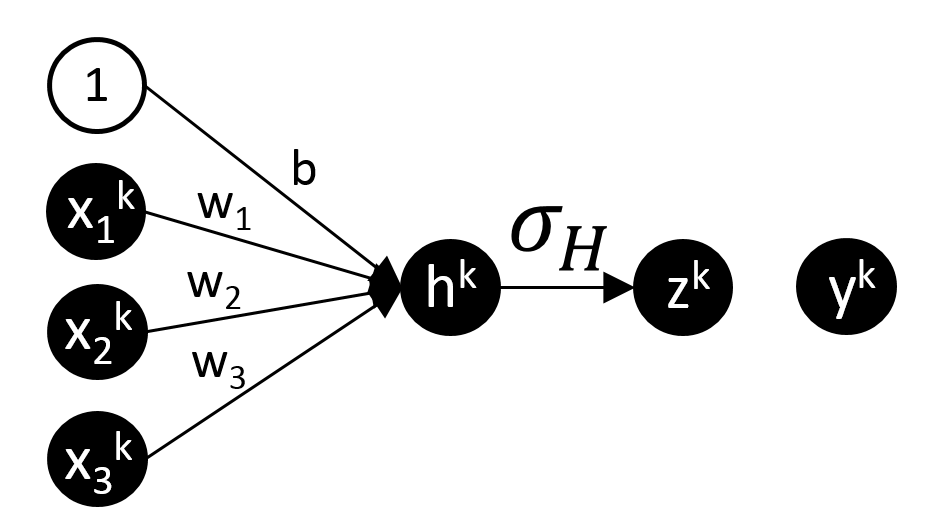
\includegraphics[width=80mm]{../../Desktop/figures/single_perceptron.PNG}
		\caption{Graphical representation of an example perceptron which predicts the output for the $k^{th}$ sample, $z^{k}$ with $\mathbf{x}^{k} 
			\in R^{3}$. The ``1" is a constant multiplier which differentiates regular weights values from the bias value $b$.}
		\label{perceptron}
	\end{figure}
	Perceptrons are linear classifiers, as can be seen from (\ref{equation:perceptron_output}). The perceptron's $k^{th}$ output, $z^{k}$, indicates whether $\mathbf{x}^{k}$ is above or below the hyperplane defined by $\mathbf{w}$ and $b$. Therefore, perceptrons cannot accurately classify data which cannot be separated by a hyperplane, meaning such problems require a more complex model.
	
	\subsection{Multiple Layers for Complex Models}
	
	An ff-ANN is a network of neurons. A perceptron is specific case of a single artificial neuron, one which contains the Heaviside step function as it's activation function. In general, neurons in ff-ANNs can contain any monotonically increasing function as the activation function. In our thesis all neurons use activation functions, $\sigma(.)$, which approximate the Heaviside step function by meeting the criteria:
	
	\begin{equation}
	\sigma(x) \in
	\begin{cases}
	]0.5,1] ,& \text{if } x > 0,\\
	[0,0.5],              & \text{otherwise}.
	\end{cases}
	\label{equation:classification_function}
	\end{equation}
	
	 Meeting this criteria for all activation functions, we can still use the concept of neurons as hyperplanes as described in the previous section for perceptrons. The hyperplane defined by a neuron with an activation function satisfying (\ref{equation:classification_function}) separates the two value ranges in (\ref{equation:classification_function}) rather than determining a simple binary output.
	 
	 An ff-ANN can contain several layers of neurons stacked on top of each other as well as several neurons per layer. By adding multiple layers, the network can learn more complex functions. The output of the neurons at each layer, which is the more general version of (\ref{equation:perceptron_output}), becomes:
	\begin{equation}
	\mathbf{z}_{l}^{k} = \sigma_{l}(\mathbf{W}_{l}\mathbf{z}_{l-1}^{k} + \mathbf{b}_{l}), \quad \text{for} \ l = 1, ... , L,
	\end{equation}
	where $l$ represents the layer number, $\sigma_{l}()$ is the activation function at layer $l$, $L$ is the total number of layers, $\mathbf{W}_{l}$ and $\mathbf{b}_{l}$ contain the weights and biases for layer $l$ where each row contains the parameters for a single neuron, and:
	\begin{equation}
	\mathbf{z}_{0}^{k} = \mathbf{x}^{k}, \quad \text{for} \ k=1, 2, ... , m.
	\end{equation}
	The final classification prediction is the output of the final layer, $\mathbf{z}_{L}^{k}$, for the $k^{th}$ training example. The purpose of having multiple layers is to model more complex non-linear functions. Considering the neurons as hyperplanes, by assuming the neurons' activation functions meet (\ref{equation:classification_function}), a neuron in the second layer then separates the results from the first layer. See Figure \ref{figure:MLP} for an example of a dataset that can be separated using a two layer network but not a single neuron, illustrated using hyperplane representations of neurons. In this example we show that a single hyperplane cannot separate the given example data, however two hyperplanes whose outputs are combined using a single hyperplane can be used to perfectly separate the data.
	\begin{figure}
		\centering
		\begin{subfigure}{.3\textwidth}
			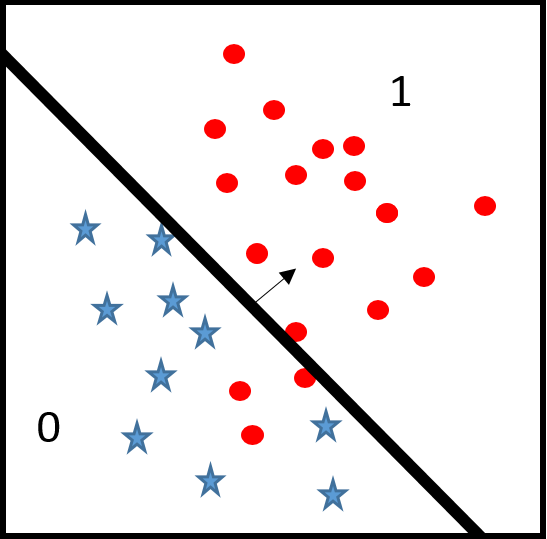
\includegraphics[width=\textwidth]{../../Desktop/figures/single_neuron.PNG}
			\caption{}
		\end{subfigure}
		\begin{subfigure}{.3\textwidth}
			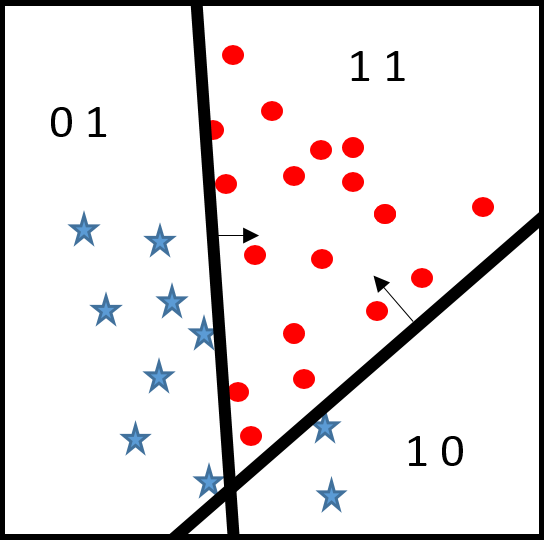
\includegraphics[width=\textwidth]{../../Desktop/figures/first_layer_2neurons.PNG}
			\caption{}
		\end{subfigure}
		\begin{subfigure}{.3\textwidth}
			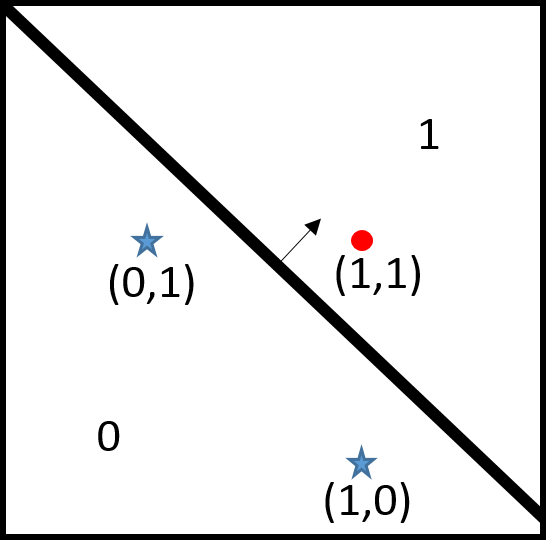
\includegraphics[width=\textwidth]{../../Desktop/figures/secon_layer_1neuron.PNG}
			\caption{}
		\end{subfigure}
		\caption{Visualization of the capacity increase from having multiple layers in a network. Subplot a) shows the classification potential for a single perceptron. Subplots b) and c) show the potential classification performed by 3 perceptrons, 2 in the first layer and 1 in the second.}
		\label{figure:MLP}
	\end{figure}
	
	
	\subsection{Training}
	
	Now that we have provided intuition for why ff-ANNs have the potential to model complex functions, we focus this section on how the parameters of a network are tuned or ``trained" to meet potential. The goal of training is to fit the network to the training data by solving an optimization problem. Typically the objective function, $f(\mathbf{W}_{1},...,\mathbf{W}_{L},\mathbf{b}_{1},...,\mathbf{b}_{L})$, used for this optimization problem is the mean squared error of the set of all $m$ training examples, which can be written as: 
	\begin{equation}
	f(\mathbf{W}_{1},...,\mathbf{W}_{L},\mathbf{b}_{1},...,\mathbf{b}_{L}) = \frac{1}{m}\sum_{k=1}^{m}{(\mathbf{y}^{k} - \mathbf{z}_{L}^{k})^{T}(\mathbf{y}^{k} - \mathbf{z}_{L}^{k})},
	\label{equation:objective_function}
	\end{equation}
	where $\mathbf{z}_{L}^{k}$ is the network's prediction for $\mathbf{y}^{k}$ which depends on weights $\mathbf{W}_{l}$ and biases $\mathbf{b}_{l}$ for all layers $l$, $l=1,...,L$. The optimization problem for training the network is therefore:
	\begin{equation}
	\begin{aligned}
	& \underset{\mathbf{W}_{1},...,\mathbf{W}_{L},\mathbf{b}_{1},...,\mathbf{b}_{L}}{\text{min}}
	& & \frac{1}{m}\sum_{k=1}^{m}{(\mathbf{y}^{k} - \mathbf{z}_{L}^{k})^{T}(\mathbf{y}^{k} - \mathbf{z}_{L}^{k})}.\\
	\end{aligned}
	\label{equation:optimization}
	\end{equation}
	The ultimate objective of training a ff-ANN, and machine learning models in general, is to maximize the accuracy of predicted dependent variable $\mathbf{z}$ for independent variable $\mathbf{x}$ that is outside of the set $S$, in addition to maintaining model accuracy for the training data in $S$. Accuracy of the model on the training set is attained through the use of a numerical optimization method. Various methods are used, each with different benefits and drawbacks. This will be discussed in \S{2.2}.
	
	\subsection{Overfitting}
	
	Overfitting describes fitting a model to a training set such that it performs poorly on unseen data compared to on the training data. In other words, the trained model does not generalize well. As previously discussed, ff-ANNs can model very complex functions. When there is a small training set, it may learn a function influenced by the noise of the training set rather than purely the signal shared by unseen and training data alike, leading to this lack of generalizability \cite{dropout}. Since many problems are tackled using machine learning where the underlying model dimensionality is not known prior to learning, we do not know how large our ff-ANN should be to prevent overfitting without over-simplifying the model. There are many techniques to avoid overfitting without shrinking the network. In our experiments we use a regularization term which penalizes large values of the parameters. It is a way to reduce the capacity of the network and therefore helps prevent overfitting. Specifically the final objective function with our added regularization term has the following form:
	\begin{equation}
	f(\mathbf{x}) = g(\mathbf{x}) + \lambda_{r}\|\mathbf{x}\|_{2}^{2},
	\label{equation:regularization}
	\end{equation}
	where $g(\mathbf{x})$ is the initial objective function, $\mathbf{x}$ is the parameters for the objective function and $f(\mathbf{x})$ is the resulting objective function when using regularization for the problem, $\lambda_{r}$ is what is known as the `regularization' parameter which tunes the level of impact of the regularization term on the original objective function and $\|\mathbf{x}\|_{2}^{2}$ is the 2-norm of the parameters, $\mathbf{x}$.
	
	\section{Optimization Methods for Training ff-ANNs}
	
	For simplicity of discussion, we consider a general unconstrained optimization problem:
	\begin{equation}
	\begin{aligned}
	& \underset{\mathbf{w}\in \mathbb{R}^{n}}{\text{min}}
	& & f(\mathbf{w}).\\
	\end{aligned}
	\label{equation:optimization_simple}
	\end{equation}
	Note that (\ref{equation:optimization}) can be transformed into the form of (\ref{equation:optimization_simple}) by adding the regularization component as in (\ref{equation:regularization}) and vectorizing parameters $\mathbf{W}_{l}$, and $\mathbf{b}_{l}$ for $l = 1,...,L$ into a single vector $\mathbf{w}$, which is discussed in Appendix \ref{appendix:forandback}.
	
	As described in \S{2.1.3}, a numerical optimization method is required to solve (\ref{equation:optimization}). A lot of work has been done in numerical optimization for ff-ANNs that can be sorted into two categories, those that use only first-order information and those that also use second-order information of an ff-ANN objective function, (\ref{equation:objective_function}). 
	
	The particular challenges for solving large ff-ANN training problems are:
	\begin{enumerate}
		\item {Large number of training examples, $m$,}
		\item {Large number of dimensions (weights, including biases), $n$. }
	\end{enumerate}
	For instance, a network with 7 layers and 100 hidden nodes per layer would have $n=70700$ ($100^{2}$ weights and $100$ biases for each layer) and the value of $m$ can be in the millions. The following characteristics of a ff-ANN objective function surface pose additional challenges to solving (\ref{equation:optimization_simple}) are \cite{Shepherd.1997}:
	\begin{enumerate}
		\item {Large plateaus (flat or nearly flat areas),}
		\item {Narrow valleys,}
		\item {Many saddle points (exponentially increasing with number of parameters, $n$).}
	\end{enumerate}
	This means that numerical optimization methods need to perform \textbf{well} on a problem with these characteristics to be considered suited for ff-ANNs. Typically the definition of \textbf{well} is based on a mixture of speed (training time), training error, prediction accuracy of test set and the final objective function value. In this thesis we will mainly focus on training time and training error.
	
	\subsection{First Order Methods}
	
	Here we will describe some common optimization methods used for training ff-ANNs using only first order information. 
	\begin{enumerate}
		\item {\textbf{Gradient Descent} is typically only used for small datasets which has the update defined by 
			\begin{equation}
			\mathbf{w}_{k} = \mathbf{w}_{k-1} - \eta{\nabla}{f(\mathbf{w}_{k-1})},
			\label{equation:gd_update}
			\end{equation}
			where $\eta$ is the learning rate. When $\eta$ is small enough and kept constant, with random initialization, gradient descent does not converge to a saddle point almost surely \cite{gd_converges.paper}.
		}
		\item{\textbf{Stochastic Gradient Descent} is a commonly known and used method which approximates gradient descent using only a single example at each step. Each iteration $i$ has the update:
			\begin{equation}
			\mathbf{w}_{k} = \mathbf{w}_{k-1} - \eta\widetilde{\nabla}{f(\mathbf{w}_{k-1})},
			\label{equation:sgd_update}
			\end{equation}
			where $\eta$ is the learning rate chosen by the user which is decreased in magnitude throughout training using a predefined schedule, and $\widetilde{\nabla}{f(\mathbf{w}_{k-1})}$ refers to the approximation of the gradient of the objective function at point $\mathbf{w}_{k-1}$ based on a single, uniformly randomly selected, training example. 
		}   
		\item{\textbf{Mini-batch Gradient Descent} is a method that uses the same update function as shown in (\ref{equation:sgd_update}) but with $\widetilde{\nabla}{f(\mathbf{w}_{k-1})}$ computed as an approximation to the gradient of the objective function at point $\mathbf{w}_{k-1}$ based on a \textbf{subset} of the set of training examples $S$.}
	\end{enumerate}
	First order methods compute steps very quickly. However, they can experience difficulties in some regions, such as in valleys. A valley is an example of a characteristic often seen in ff-ANN problems \cite{Shepherd.1997} that slows down first order methods. First order methods experience difficulties in this case because the gradient direction is almost perpendicular to the direction of the local minimum. Figure \ref{figure:valley}, which is from \cite{martens2010deep}, depicts this concept. These gradient methods also have difficulties in small gradient areas such as large pseudo-plateaus, since the length of the step taken at each iteration is proportionate to the size of the gradient for a constant learning rate.
	
	\begin{figure}[h]
		\centering
		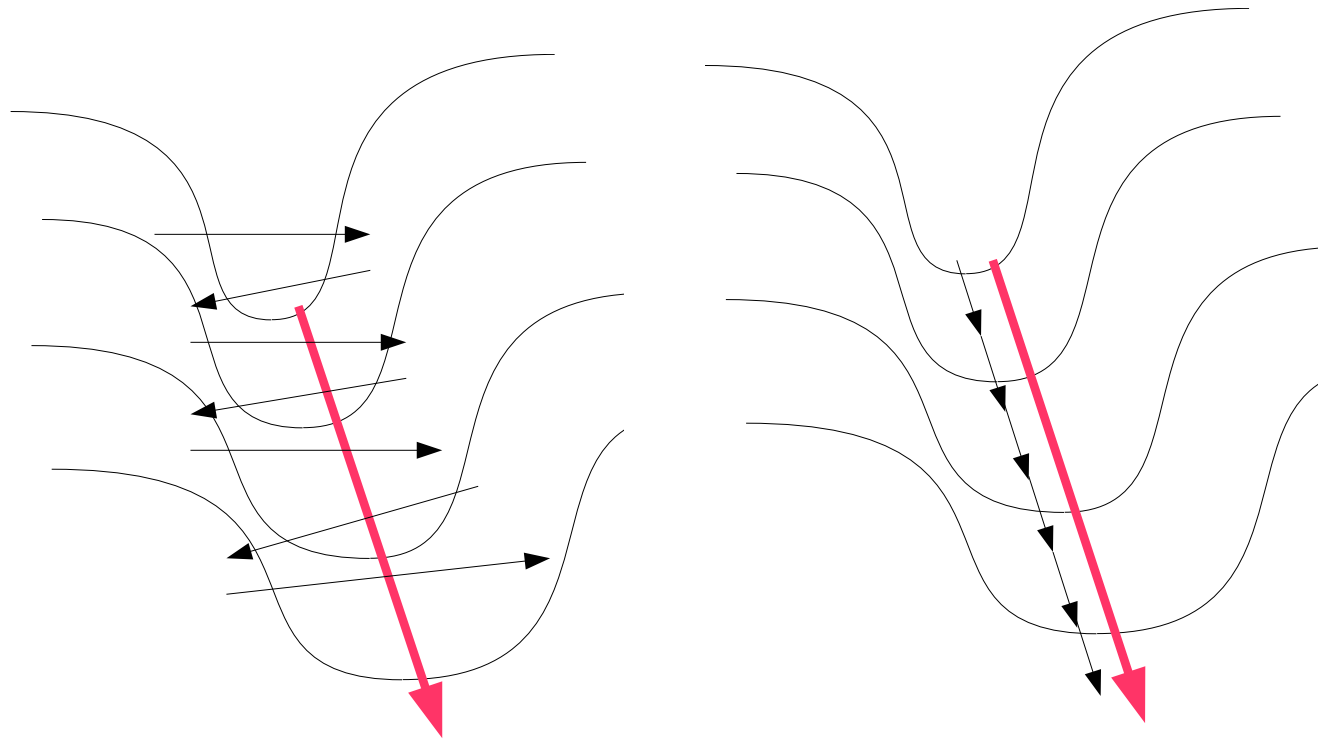
\includegraphics[width=0.5\linewidth]{../../Desktop/figures/Deeplearning_HF_valley.PNG}
		\caption{This is Figure 1 from \cite{martens2010deep} which shows an example of a valley characteristic. On the left the arrows point towards the gradient direction and the red arrow points towards the shortest path to the smallest value visible. On the right are arrows pointing in the direction of a method considering curvature and therefore avoiding the gradient direction which is, in this case, in a direction of high positive curvature.}
		\label{figure:valley}
	\end{figure}
	
	\subsection{Second Order Methods} \label{section:second_order}
	
	The first group of methods presented below are approximate second order methods which are faster to compute and do not contain exact second order information. Instead, they estimate Hessian information using various approaches. Some examples are:
	
	\begin{enumerate}
		\item{\textbf{Quasi-Newton methods} estimate the Hessian matrix (second order information) using only first order derivatives. The full Newton's method updates the iterate as follows:
			\begin{equation}
			\mathbf{w}_{k} = \mathbf{w}_{k-1} - (\nabla^{2}{f(\mathbf{w}_{k-1})})^{-1}\nabla{f(\mathbf{w}_{k-1})},
			\label{equation:newtons}
			\end{equation}
			where $\nabla^{2}{f(\mathbf{w}_{k-1})}$ is the Hessian matrix of $f(
			\mathbf{w}_{k-1})$. This step is the solution to the first order critical point of the second order approximation of $f(\mathbf{w}_{k-1})$ using the Taylor series expansion, (\ref{equation:taylor_series}). Quasi-Newton methods replace $(\nabla^{2}{f(\mathbf{w}_{k-1})})$ with an approximation to the Hessian. A common quasi-Newton method is the \textbf{BFGS (Broyden-Fletcher-Goldfarb-Shanno) algorithm} which approximates the Hessian using the secant equation \cite{Shepherd.1997}.  
		}
		\item{\textbf{Finite Difference Newton Methods} are methods where $(\nabla^{2}{f(\mathbf{w}_{k-1})})$ in (\ref{equation:newtons}) is replaced by a finite difference approximation to the Hessian which uses only first order information \cite{Shepherd.1997}.}
		\item{\textbf{Levenberg-Marquardt} is an algorithm for non-linear least squares problems, which has an update of the following form \cite{Shepherd.1997}:
			\begin{equation}
			\mathbf{w}_{k} = \mathbf{w}_{k-1} + [\mathbf{J}^{T}_{k-1}\mathbf{J}^{}_{k-1} + \lambda\mathbf{I}]^{-1}\mathbf{J}^{T}_{k-1}\mathbf{r}_{k-1}.
			\end{equation}    
			Here $\mathbf{r}_{k-1}$ is the residual vector which contains values $(\mathbf{y}^{k} - \mathbf{z}_{L}^{k})_{i}$ for all indices $i=1,...,n_{L}$ where $\mathbf{y}^{k} \in \mathbb{R}^{n_{L}}$, and all training examples $k = 1,...,m$, identified by the superscript. The iteration index is $k-1$, identified by the subscript. The matrix $\mathbf{J}_{k-1}$ is the Jacobian of $\mathbf{r}_{k-1}$ in terms of each weight, and $\lambda$ is a damping factor which is adapted based on descent speed \cite{Shepherd.1997}. }    
	\end{enumerate}
	These methods are quite effective at approximating curvature in many instances without the computational time cost of actually computing it directly. BFGS in particular is a very well known approach for incorporating second order information based on recent updates. These, however, do not have the full second order information, e.g., the negative curvature information may be absent in the Hessian update. There are also methods that use exact second order information which we are interested in for this thesis. 
	\begin{enumerate}
		\item{\textbf{Newton's Method} is a classical second order optimization method which is only locally convergent. The Newton's method update is defined by (\ref{equation:newtons}). This method is the inspiration for some  second order methods for neural network learning such as the ``Approximate saddle-free Newton" method proposed by \cite{saddle_free}.}
		\item{\textbf{Trust Region Methods} are globally convergent methods. At each iteration a solution to a subproblem which approximates the original problem, in a trusted region, based on the first and second order information of the objective function, is used to determine a step towards the solution for the original problem. This is the approach we focus on for this thesis. }
	\end{enumerate}
	We specifically investigate a trust region method with exact Hessian information in this thesis as well as modified versions based on subsampling of parameters and training examples. Part of our motivation in looking at trust region methods is that they are well suited to non-convex problems since a global minimizer to the subproblem is computed at each iteration. This does not mean a global minimizer will be computed for the problem but does lead to convergence to a local minimizer. 
	
	\section{Trust Region Methods}
	The idea of a trust region method is to solve a subproblem at each iteration based on a model that is trusted within a certain radius around the current point. Trust region methods consist of the following steps \cite{TRM.book}:
	\begin{enumerate}
		\item {Subproblem definition.} \label{model def}
		\item {Step calculation: solving the ``Trust Region Subproblem".} \label{step calc}
		\item {Acceptance of the trial point.} \label{accept step}
		\item {Trust-region radius update.} \label{update radius}
	\end{enumerate}
	In this section we will go through each step and specify the approach that will be used in our numerical exploration. Initialization specifies a guess for solution $\mathbf{w}$. In our investigation, the initial guess is uniformly pseudo-random values in the range of [-0.5,0.5]. The weight matrices, $\mathbf{W}_{l}$ at each layer $l$, are then normalized by dividing each matrix by the sum of the absolute value of all their matrix elements. 
	
	\subsection{Subproblem Definition}
	
	Trust region methods typically use a quadratic approximation as the model for the objective function, $f(\mathbf{w})$. At the current iterate, the second order approximation to the objective function, $f(\mathbf{w} + \mathbf{p})$ is:
	
	\begin{equation}
	\begin{split}
	\tilde{f}(\mathbf{w} + \mathbf{p}) =  &f(\mathbf{w}) + \nabla f(\mathbf{w})^{T}\mathbf{p} + \frac{1}{2}\mathbf{p}^{T}\nabla^{2} f(\mathbf{w})\mathbf{p} \\
	= & f(\mathbf{w}) + \mathbf{g}^{T}\mathbf{p} + \frac{1}{2}\mathbf{p}^{T}\mathbf{H}\mathbf{p}, 
	\end{split}
	\label{equation:taylor_series}
	\end{equation}
	where $\mathbf{p}$ is the step (change in parameter values) we wish to find, $\mathbf{w}$ is the current parameter vector of the function $f$, $\mathbf{g}=\nabla f(\mathbf{w})$ is the gradient and $\mathbf{H}= \nabla^{2} f(\mathbf{w})$ is the Hessian matrix at $\mathbf{w}$. 
	
	In this thesis $\mathbf{H}$ denotes the exact Hessian rather than an approximation, which is common among numerical methods for ff-ANNs as discussed in \S{\ref{section:second_order}}. 
	
	%======================================================================
	\subsection{Step Calculation: Solving the Trust Region Subproblem}
	%======================================================================
	
	The step calculation of a trust region method computes the minimizer of the quadratic approximation within a trust region \cite{TRM.book} formally written as:
	\begin{equation}
	\begin{aligned}
	& \underset{\mathbf{p}}{\text{min}}
	& & \mathbf{g}^{T}\mathbf{p} + \frac{1}{2}\mathbf{p}^{T}\mathbf{Hp} \\
	& \text{s.t.}
	& & \mathbf{p}^{T}\mathbf{p} \leq \gamma^{2},
	\label{equation:TRS}
	\end{aligned}
	\end{equation}
	where $\gamma$ is the radius of the trusted region. Throughout this thesis, we will refer to the objective function of the trust region subproblem as $\delta(\mathbf{p})$, therefore:
	\begin{equation}
	\delta(\mathbf{p}) = \mathbf{g}^{T}\mathbf{p} + \frac{1}{2}\mathbf{p}^{T}\mathbf{Hp}.
	\label{equation:delta}
	\end{equation}
	
	Traditionally, the trust region subproblem is solved using an iterative method involving repeatedly computing solutions to linear equations or eigenvalue problems. It is demonstrated in a recent paper, \cite{adachi.paper}, that the trust region subproblem can be solved by a single generalized eigenvalue problem and linear equation. This makes the trust region method more appealing since it is simple to implement with the possibility of improved computational efficiency. We provide the details of this computation.  
	
	\subsubsection{Optimality Conditions}
	
	In this section we present and explain the optimality conditions for the solution to the trust region subproblem (TRS), (\ref{equation:TRS}), for the simple case when the solution is unique. The TRS is a special example of a non-convex problem with strong duality \cite{boyd}. A solution to the dual problem is the Lagrangian multiplier which can be used to compute the solution to the primal problem. In the following section we will derive the optimality conditions for the TRS using the strong duality property of the problem. Firstly, in order to satisfy primal feasibility (\ref{equation:TRS}), we have:
	\begin{equation}
	\mathbf{p}^{T}\mathbf{p} \leq \gamma^2.
	\label{equation:inbounds}
	\end{equation}
	The Lagrangian function of (\ref{equation:TRS}) is:
	\begin{equation}
	\begin{split}
	\mathcal{L}(\mathbf{p},\lambda) = &\mathbf{g}^{T}\mathbf{p} + \frac{1}{2}\mathbf{p}^{T}\mathbf{Hp} + \frac{1}{2}\lambda (\mathbf{p}^{T}\mathbf{p} - \gamma^{2}),\\ = &\mathbf{g}^{T}\mathbf{p} + \frac{1}{2}\mathbf{p}^{T}(\mathbf{H} + \lambda\mathbf{I})\mathbf{p} - \frac{1}{2}\lambda\gamma^{2},
	\label{equation:lagrangian}
	\end{split}
	\end{equation}
	where $\lambda$ is the Lagrange multiplier. To satisfy complimentary slackness, $\lambda$ and $\mathbf{p}$ must satisfy:
	\begin{equation}
	\lambda(\mathbf{p}^{T}\mathbf{p} - \gamma^{2}) = 0.
	\label{equation:complementary_slackness}
	\end{equation}
	The dual function becomes:
	\begin{equation}
	\begin{aligned}
	d(\lambda) & = \underset{\mathbf{p}}{\inf}
	\ \mathcal{L}(\mathbf{p},\lambda)  \\
	& = -\frac{1}{2}\lambda\gamma^{2} + \underset{\mathbf{p}}{\inf}
	\ (\mathbf{g}^{T}\mathbf{p} + \frac{1}{2}\mathbf{p}^{T}(\mathbf{H} + \lambda\mathbf{I})\mathbf{p}). \\
	\label{equation:dual}
	\end{aligned}
	\end{equation}
	The infimum of the quadratic function in (\ref{equation:dual}) is $-\infty$ when $(\mathbf{H} + \lambda\mathbf{I})$ is indefinite. For a value of $\lambda$ such that $(\mathbf{H} + \lambda\mathbf{I})$ is singular we refer the reader to the ``hard case" described in \cite{adachi.paper}.  When $(\mathbf{H} + \lambda\mathbf{I}) \succ \mathbf{0}$ we can compute $d(\lambda)$ by computing the first order stationary point of $\mathcal{L}(\mathbf{p},\lambda)$ in terms of $\mathbf{p}$, which, given positive definiteness of $(\mathbf{H} + \lambda\mathbf{I})$, means that this is a global minima of (\ref{equation:lagrangian}) in terms of $\mathbf{p}$. The first order condition gives us:
	\begin{equation}
	\begin{aligned}
	\nabla_{\mathbf{p}} \mathcal{L}(\mathbf{p},\lambda) & = \mathbf{g} + (\mathbf{H} + \lambda\mathbf{I}) \mathbf{p} = \mathbf{0} \\
	& \rightarrow (\mathbf{H} + \lambda\mathbf{I})\mathbf{p} = -\mathbf{g}.
	\end{aligned}
	\label{equation:grad_lagrangian}
	\end{equation}
	We can now simplify the infimum from (\ref{equation:dual}) by using (\ref{equation:grad_lagrangian}) and assuming ($\mathbf{H} + \lambda\mathbf{I}) \succ \mathbf{0}$:
	\begin{equation}
	\begin{aligned}
	\underset{\mathbf{p}}{\inf}
	&(\mathbf{g}^{T}\mathbf{p} + \frac{1}{2}\mathbf{p}^{T}(\mathbf{H} + \lambda\mathbf{I})\mathbf{p}) \\ & \quad = -\mathbf{g}^{T}(\mathbf{H} + \lambda\mathbf{I})^{-1}\mathbf{g} + \frac{1}{2}\mathbf{g}^{T}(\mathbf{H} + \lambda\mathbf{I})^{-1}(\mathbf{H} + \lambda\mathbf{I})(\mathbf{H} + \lambda\mathbf{I})^{-1}\mathbf{g}   \\
	& \quad = -\mathbf{g}^{T}(\mathbf{H} + \lambda\mathbf{I})^{-1}\mathbf{g} + \frac{1}{2}\mathbf{g}^{T}(\mathbf{H} + \lambda\mathbf{I})^{-1}\mathbf{g} \\
	& \quad = - \frac{1}{2}\mathbf{g}^{T}(\mathbf{H} + \lambda\mathbf{I})^{-1}\mathbf{g}.
	\end{aligned}
	\label{equation:infimum}
	\end{equation}
	 Using (\ref{equation:infimum}) to simplify (\ref{equation:dual}), the dual function, we get:
	\begin{equation}
	d(\lambda)= 
	-\frac{1}{2}\lambda\gamma^{2} - \frac{1}{2}\mathbf{g}^{T}(\mathbf{H} + \lambda\mathbf{I})^{-1}\mathbf{g},
	\label{equation:dual2}
	\end{equation}
	 for values of $\lambda$ such that:
	\begin{equation}
	(\mathbf{H} + \lambda\mathbf{I}) \succ \mathbf{0}.
	\label{equation:possemdef}
	\end{equation}
	 The remaining discussion is on a technique by Adachi et al \cite{adachi.paper} to determine the value of $\lambda$ which maximizes (\ref{equation:dual2}). A stationary point must satisfy:
	\begin{equation}
	\begin{aligned}
	d^{\prime}(\lambda)) & = \frac{1}{2} ( -\gamma^{2} + \mathbf{g}^{T}(\mathbf{H} + \lambda\mathbf{I})^{-2}\mathbf{g}) \\ & = 0. \\
	\end{aligned}
	\label{equation:grad_d}
	\end{equation}
	Using the eigenvalue decomposition for $\mathbf{H}$,
	\begin{equation}
	\mathbf{H} = \mathbf{V}^{T}\mathbf{D}\mathbf{V},
	\end{equation}
	where $\mathbf{D}$ is the diagonal matrix such that $\mu_{i} = \mathbf{D}_{ii}$ is the $i^{th}$ eigenvalue of $\mathbf{H}$ by decreasing algebraic size (ie $\mu_{1}$ is the largest eigenvalue of $\mathbf{H}$), and $\mathbf{V}$ is the matrix of eigenvectors where $\mathbf{V}_{i}$, the $i^{th}$ column vector of \textbf{V}, is the eigenvector corresponding to $\mu_{i}$. We can now write (\ref{equation:grad_d}) as:
	\begin{equation}
	\begin{aligned}
	2d^\prime(\lambda) & = -\gamma^{2} + \mathbf{g}^{T}(\mathbf{V}^{T}(\mathbf{D} + \lambda\mathbf{I})\mathbf{V})^{-2}\mathbf{g} \\
	& = -\gamma^{2} + \mathbf{g}^{T}(\mathbf{V}^{T}(\mathbf{D} + \lambda\mathbf{I})\mathbf{V}\mathbf{V}^{T}(\mathbf{D} + \lambda\mathbf{I})\mathbf{V})^{-1}\mathbf{g}  \\
	& = -\gamma^{2} + \mathbf{g}^{T}(\mathbf{V}^{T}(\mathbf{D} + \lambda\mathbf{I})(\mathbf{D} + \lambda\mathbf{I})\mathbf{V})^{-1}\mathbf{g}  \\ 
	& = -\gamma^{2} + \mathbf{g}^{T}(\mathbf{V}^{T}(\mathbf{D} + \lambda\mathbf{I})^{2}\mathbf{V})^{-1}\mathbf{g}  \\ 
	& = -\gamma^{2} + \mathbf{g}^{T}\mathbf{V}(\mathbf{D} + \lambda\mathbf{I})^{-2}\mathbf{V}^{T}\mathbf{g} \\
	& = -\gamma^{2} + \sum_{i=1}^{n}{\frac{(\mathbf{g}^{T}\mathbf{V}_{i})^{2}}{(\mu_{i} + \lambda)^{2}}} = 0\\ 
	&  \rightarrow \sum_{i=1}^{n}{\frac{(\mathbf{g}^{T}\mathbf{V}_{i})^{2}}{(\mu_{i} + \lambda)^{2}}} = \gamma^{2}.
	\end{aligned}
	\label{equation:grad_lagrangian2}
	\end{equation}
	We define $\phi(\lambda)$ as:
	\begin{equation}
	\phi(\lambda) = \sum_{i=1}^{n}{\frac{(\mathbf{g}^{T}\mathbf{V}_{i})^{2}}{(\mu_{i} + \lambda)^{2}}}.
	\label{phi}
	\end{equation}
	Now, note that $(\mu_{i} + \lambda)$ is the $i^{th}$ eigenvalue of $(\mathbf{H} + \lambda\mathbf{I})$ so in order to satisfy the requirement in (\ref{equation:possemdef}), $\mu_{n} + \lambda > 0$ where $\mu_{n}$ is the smallest eigenvalue of the Hessian matrix, $\mathbf{H}$. The $\lambda$ which fulfills this constraint as well as (\ref{equation:grad_lagrangian2}), exists and is unique when $\mathbf{g}^{T}\mathbf{V}_{n}\neq0$ since the value of $\phi(\lambda)$ is $\infty$ when $-\lambda = \mu_{n}$ and then always decreasing for $\lambda > |\mu_{n}|$ and approaches zero. A visualization of $\phi(\lambda)$ can be seen in \cite{TRM.book}, Figure 7.3.2. There is a case where the value of $\lambda$ which maximizes (\ref{equation:dual2}) makes ($\mathbf{H}+\lambda\mathbf{I}$) semi-positive definite and singular which is discussed in \cite{adachi.paper}. 

	To summarize, in order for a solution $\mathbf{p}$ to be optimal in the case that ($\mathbf{H} + \lambda\mathbf{I}) \succ \mathbf{0}$, it must satisfy primal feasibility, (\ref{equation:inbounds}), (\ref{equation:possemdef}), and complementary slackness, (\ref{equation:complementary_slackness}). Now that we have established optimality conditions for the TRS, we need to determine how to compute a solution that satisfies these conditions. The dual problem (\ref{equation:dual2}) can be solved by an iterative method to determine a solution to $\phi(\lambda) = \gamma^{2}$ where $\mathbf{H} + \lambda \mathbf{I} \succ 0$. For example, \cite{TRM.book}, finds a model minimizer using a numerical approach of adjusting $\lambda$ and solving for (\ref{equation:grad_lagrangian}) and re-adjusting $\lambda$ until a suitable $\mathbf{p}$ is achieved. As previously mentioned, in this thesis we follow a more recent approach by \cite{adachi.paper} which, for the boundary case, developed a generalized eigenvalue problem with a solution from which a solution to the TRS can be directly computed. It also takes advantage of complementary slackness to devise a two step approach described in the following section. 
	
	\subsubsection{Solving TRS via a Generalized Eigenvalue Problem}
	
	The method proposed by \cite{adachi.paper} uses a two pronged approach. They compute two steps, $\mathbf{p}_{1}$ and $\mathbf{p}_{0}$ where $\mathbf{p}_{1}$ is the optimal step for the trust region subproblem when (\ref{equation:inbounds}) is an active constraint, and $\mathbf{p}_{0}$ is a point such that $\nabla\delta(\mathbf{p}_{0}) = 0$ where $\delta(.)$ is defined by (\ref{equation:delta}). If $\mathbf{p}_{0}$ is a feasible solution, meaning (\ref{equation:inbounds}) is satisfied, then $\mathbf{p}$ is the step, out of $\mathbf{p}_{1}$ and $\mathbf{p}_{0}$, which produces the lower objective function value of the TRS, $\delta(\mathbf{w + p})$. This decision is presented as Algorithm \ref{algorithm:trialpoint}.
	
	Here we describe the details of the two parts of the method proposed in \cite{adachi.paper} as well as some explanation to show that this solution does, in fact, correspond to 
	a solution to the TRS, (\ref{equation:TRS}). For further details on the derivation of this approach we refer a reader to \cite{adachi.paper}. 
	
	\subsubsection{Interior Case}
	
	If a solution to (\ref{equation:TRS}) is in the interior then the following must be satisfied:
	\begin{subequations}
		\begin{align}
		\quad \mathbf{Hp} = & -\mathbf{g}, \label{equation:p0} \\
		\quad \mathbf{H} \succeq & \ \mathbf{0},\label{equation:p0_posdef} \\ 
		||\mathbf{p}|| < & \ \gamma, \label{equation:p0_bounds}  
		\end{align}
	\end{subequations}
	adapted from (\ref{equation:grad_lagrangian}), (\ref{equation:possemdef}) and (\ref{equation:inbounds}) respectively for this case, since $\lambda = 0$ in order to satisfy complementary slackness, (\ref{equation:complementary_slackness}).
	
	Define $\mathbf{p}_{0}$ to be a solution to (\ref{equation:p0}), which is unique when $\mathbf{H}$ is non-singular. If $\mathbf{H}$ is singular any of the feasible solutions can be submitted as the $\mathbf{p}_{0}$ solution. In the case where the hyperplane of optimal solutions intersects the trust region sphere, there will be at least one boundary case solution. Otherwise none of the possible solutions to $\mathbf{p}_{0}$ would satisfy (\ref{equation:p0_bounds}) and would therefore not be valid steps. Because of this, we can ensure that there is always a boundary solution which is a global minimizer in the case that $\mathbf{H}$ is singular. In our approach we do not check for singularity. Rather, we set a maximum number of iterations on our linear equation solver, which is the conjugate gradient method as will be discussed in the following chapter, and only consider solutions that satisfy the all of the above equations. 
	
	\subsubsection{Boundary Case via a Generalized Eigenvalue Problem}
	
	If a solution is on the boundary then it satisfies (\ref{equation:possemdef}), (\ref{equation:grad_lagrangian}), and:
	\begin{equation}
	\mathbf{p}^{T}\mathbf{p} = \gamma^{2}.
	\label{equation:boundary}
	\end{equation}
	We define $\mathbf{p}_{1}$ to be the vector that satisfies these conditions. In order to compute $\mathbf{p}_{1}$, \cite{adachi.paper} formulated a generalized eigenvalue problem such that $\mathbf{p}_{1}$ can be computed based on the eigenvalue, $\lambda_{*}$, and associated eigenvector:
	\begin{equation}
	\mathbf{v} = \begin{bmatrix}\mathbf{v}_{1} \\ \mathbf{v}_{2} \end{bmatrix}.
	\end{equation}
	where $\mathbf{v}_{1} \in \mathbb{R}^{n}$, $\mathbf{v}_{2} \in \mathbb{R}^{n}$, together with $\lambda_{*}$, satisfy:
	\begin{equation}
	\begin{bmatrix}
	-\mathbf{I} & \mathbf{H} \\
	\mathbf{H} & -\mathbf{gg}^{T}/\gamma^{2}
	\end{bmatrix}
	\begin{bmatrix}
	\mathbf{v}_{1} \\
	\mathbf{v}_{2} 
	\end{bmatrix}
	= -\lambda_{*}
	\begin{bmatrix}
	\mathbf{0} & \mathbf{I} \\
	\mathbf{I} & \mathbf{0}
	\end{bmatrix}
	\begin{bmatrix}
	\mathbf{v}_{1} \\
	\mathbf{v}_{2} 
	\end{bmatrix},
	\label{equation:M_def}
	\end{equation}
	and $\lambda_{*}$ is the largest eigenvalue satisfying this equation. We define the lefthand side of (\ref{equation:M_def}) to be matrix $\mathbf{M}$ for simplicity. That is:
	\begin{equation}
	\mathbf{M} = 
	\begin{bmatrix}
	-\mathbf{I} & \mathbf{H} \\
	\mathbf{H} & -\mathbf{gg}^{T}/\gamma^{2}.
	\end{bmatrix}
	\label{equation:M}
	\end{equation}
		
	The paper by Adachi et al \cite{adachi.paper} states that the optimal boundary solution is:
	\begin{equation}
	\mathbf{p}_{1} = - \frac{\gamma^{2}}{\mathbf{g}^{T}\mathbf{v}_{2}}\mathbf{v}_{1}.
	\label{equation:p1}
	\end{equation}
	We can verify this by checking that the optimality conditions are satisfied. Firstly, we re-write (\ref{equation:M_def}) as two equations:
	\begin{equation}
	-\mathbf{v}_{1} + \mathbf{H}\mathbf{v}_{2} = -\lambda_{*}\mathbf{v}_{2},
	\label{equation:M_def1}
	\end{equation}
	and
	\begin{equation}
	\mathbf{H}\mathbf{v}_{1}-\mathbf{gg}^{T}\mathbf{v}_{2}/\gamma^{2} = -\lambda_{*}\mathbf{v}_{1}.
	\label{equation:M_def2}
	\end{equation}
	Rearranging (\ref{equation:M_def2}) we get:
	\begin{equation}
	(\mathbf{H} + \lambda_{*}\mathbf{I})(- \frac{\gamma^{2}}{\mathbf{g}^{T}\mathbf{v}_{2}}\mathbf{v}_{1}) = -\mathbf{g},
	\label{equation:M_def2_rearranged}
	\end{equation}
	which is equivalent to (\ref{equation:grad_lagrangian}) with the RHS of (\ref{equation:p1}) replaced by $\mathbf{p}_{1}$. Therefore the dual feasibility, (\ref{equation:grad_lagrangian}), is satisfied. Rearranging (\ref{equation:M_def1}) we get:
	
	\begin{equation}
	\mathbf{v}_{1} = (\mathbf{H} + \lambda_{*}\mathbf{I})\mathbf{v}_{2}.
	\label{equation:v1v2}
	\end{equation}
	Now we are able to show that $\mathbf{p}_{1}$ satisfies (\ref{equation:boundary}):
	\begin{align*}
	\mathbf{p}_{1}^{T}\mathbf{p}_{1} =  & (- \frac{\gamma^{2}}{\mathbf{g}^{T}\mathbf{v}_{2}}\mathbf{v}_{1})^{T}(- \frac{\gamma^{2}}{\mathbf{g}^{T}\mathbf{v}_{2}}\mathbf{v}_{1}) & \text{using (\ref{equation:p1})},\\
	= & \frac{\gamma^{4}}{(\mathbf{g}^{T}\mathbf{v}_{2})^{2}}\mathbf{v}_{1}^{T}\mathbf{v}_{1}, \\
	= & \frac{\gamma^{4}}{(\mathbf{g}^{T}\mathbf{v}_{2})^{2}}\mathbf{v}_{2}^{T}(\mathbf{H} + \lambda_{*}\mathbf{I})^{T}\mathbf{v}_{1} & \text{using (\ref{equation:v1v2}),} \\ 
	= & \frac{\gamma^{4}}{(\mathbf{g}^{T}\mathbf{v}_{2})^{2}}\mathbf{v}_{2}^{T}(\mathbf{g}\frac{\mathbf{g}^{T}\mathbf{v}_{2}}{\gamma^{2}}) & \text{using (\ref{equation:M_def2_rearranged})},\\
	= & \frac{\gamma^{4}}{(\mathbf{g}^{T}\mathbf{v}_{2})^{2}}\frac{(\mathbf{g}^{T}\mathbf{v}_{2})^{2}}{\gamma^{2}}, \\
	= &\gamma^{2}.
	\end{align*}
	The condition (\ref{equation:possemdef}) is satisfied by taking the eigenvalue/eigenvector pair of (\ref{equation:M_def}) with the eigenvalue of the largest algebraic value which is explained in \cite{adachi.paper}. In the case where $(\mathbf{H} + I\lambda_{*})$ is singular, we have what is considered the ``hard case" which rarely occurs. See \cite{adachi.paper} for an approach to dealing with this case.  
	
	\subsubsection{Choosing the trial point}
	
	The trial point $\mathbf{p}$ is chosen based on the decision as described in Algorithm \ref{algorithm:trialpoint} which considers both $\mathbf{p}_{0}$ and $\mathbf{p}_{1}$ to determine the global minimizer, $\mathbf{p}$, to (\ref{equation:TRS}).
	\begin{algorithm}
		\caption{Selecting Global Minimizer, $\mathbf{p}$, to (\ref{equation:TRS})}\label{algorithm:trialpoint}
		\begin{algorithmic}[1]
			\State $\delta(.)$ from (\ref{equation:delta}), $\mathbf{w}$ and $\gamma$ are known
			\If {$||\mathbf{p}_{0}|| \leq \gamma \text{ and } \delta(\mathbf{p}_{0}) < \delta(\mathbf{p}_{1})$}
			\State {$\mathbf{p} \gets \mathbf{p}_{0}$}
			\Else {}
			\State $\mathbf{p} \gets \mathbf{p}_{1}$
			\EndIf 
		\end{algorithmic}
	\end{algorithm}
	
	\subsection{Acceptance of the trial point}
	
	In order to determine the acceptability of the step, as well as adjust the trust region size adaptively, we use a ratio $\rho$ defined as:
	\begin{equation}
	\rho = \frac{f(\mathbf{w} + \mathbf{p}) - f(\mathbf{w})}{\delta(\mathbf{p})},
	\label{equation:rho}
	\end{equation}
	which is the ratio of true change in objective function to the estimated objective function value change based on our model, $\delta(\mathbf{p})$, defined by (\ref{equation:delta}). 
	
	We follow the method presented in Fletcher (1987) \cite{Fletcher.1987} where a parameter, we refer to as $lb$, that satisfies $0 < lb < 1$, is used as the threshold for whether or not the step leads to a sufficient decrease in the objective function. This decision is presented as Algorithm \ref{algorithm:accept_trial_point}.
	
	\begin{algorithm}
		\caption{Acceptance of the trial point \cite{Fletcher.1987}}\label{algorithm:accept_trial_point}
		\begin{algorithmic}[1]
			\State $lb \in (0,1)$
			\State compute $\rho$ using (2.21)
			\If{$\rho \geq lb$}
			\State $\mathbf{w} \gets \mathbf{w} + \mathbf{p}$
			\Else
			\State $\mathbf{w} \text{ is unchanged}$
			\EndIf
		\end{algorithmic}
	\end{algorithm}
	
	\subsection{Trust region radius update}
	
	In this section we describe the method in \cite{Fletcher.1987} for adaptive adjustment of the trust region radius, $\gamma$. This update method is presented in Algorithm \ref{trust region size}. In this method we use two parameters $ub$ and $lb$ where $lb$ is the same value as in Algorithm \ref{algorithm:accept_trial_point} and $ub$ is used to determine when the trusted region can be expanded. These parameters must satisfy:
	\begin{equation}
	0 < lb < ub < 1.
	\label{equation:lbub}
	\end{equation}
	Conceptually this algorithm increases the radius of the trusted area when the model at the previous step is deemed very accurate, $\rho > ub$, shrink it if it was deemed insufficiently accurate, $\rho < lb$, and keep it constant otherwise. The shrinking is controlled by a parameter, $\alpha_{s}$ where $0 < \alpha_{s} < 1$, and the growth is controlled by a parameter $\alpha_{g} > 1$. When $\mathbf{w}$ is kept constant, $\mathbf{g}$ and $\mathbf{H}$ remain unchanged and can be re-used for the next iteration, reducing computation time. 
	\begin{algorithm}
		\caption{Adaptive adjustment of trust region size}\label{trust region size}
		\begin{algorithmic}[1]
			\State $lb$, $ub$, $\alpha_{g}$ and $\alpha_{s}$ are given where $lb$ and $ub$ satisfy (\ref{equation:lbub}), $\alpha_{g} > 1$ and $0 < \alpha_{s} < 1$
			\State compute $\rho$ using (2.21)
			\If{$\rho < lb$}
			\State $\gamma \gets \gamma\alpha_{s}$
			\ElsIf{$\rho > ub$}
			\State $\gamma = \max(\gamma,\alpha_{g}||\mathbf{p}||)$
			\EndIf
		\end{algorithmic}
	\end{algorithm}
	
	\subsection{Method Summary}
	For clarity and the reader's reference, we present the full trust region algorithm used in this thesis in Algorithm \ref{trust region method} which combines all steps described in this section and includes the stopping criteria, e.g. stopping when $||\mathbf{g}|| > 10^{-8}$.
	\begin{algorithm}
		\caption{Full Trust Region Algorithm to Solve (\ref{equation:optimization_simple})}\label{trust region method}
		\begin{algorithmic}[1]
			\State $lb$, $ub$, $\alpha_{g}$ and $\alpha_{s}$ are given where $lb$ and $ub$ satisfy (\ref{equation:lbub}), $\alpha_{g} > 1$ and $0 < \alpha_{s} < 1$
			\State $\mathbf{w}$ $\gets$ initialized randomly 
			\State $\gamma \gets 1$
			\While{$||\mathbf{g}|| > 10^{-8}$}
			\If{$\mathbf{w}$ was updated on the previous iteration}
			\State $\mathbf{g}$, $\mathbf{H}$ $\gets$ computed based on $\mathbf{w}$
			\State compute $\mathbf{p}_{0}$ s.t. $\mathbf{Hp}_{0} = -\mathbf{g}$
			\EndIf
			\State compute $\mathbf{p}_{1}$ from (\ref{equation:p1}) 
			\If {$||\mathbf{p}_{0}|| \leq \gamma \text{ and } \delta(\mathbf{p}_{0}) < \delta(\mathbf{p}_{1})$}
			\State {$\mathbf{p} \gets \mathbf{p}_{0}$}
			\Else {}
			\State $\mathbf{p} \gets \mathbf{p}_{1}$
			\EndIf 
			\State compute $f(\mathbf{w} + \mathbf{p})$ and $\delta(\mathbf{p})$ 
			\State compute $\rho$ from (\ref{equation:rho})
			\If{$\rho < lb$}
			\State $\gamma \gets \gamma\alpha_{s}$
			\Else{}
			\State $\mathbf{w} \gets \mathbf{w} + \mathbf{p} $
			\If{$\rho > ub$}
			\State $\gamma = \max(\gamma,\alpha_{g}||\mathbf{p}||)$
			\EndIf
			\EndIf
			\EndWhile
			\State return $\mathbf{w}$
		\end{algorithmic}
	\end{algorithm}
	
	
	%----------------------------------------------------------------------
	\chapter{Solving the Trust Region Subproblem for Feedforward Neural Networks}
	%----------------------------------------------------------------------
	In the previous chapter we discussed trust region methods and an approach to solving the trust region subproblem by using a generalized eigenvalue problem proposed by Adachi et al. \cite{adachi.paper}. In this chapter we will propose a complete algorithm for using the trust region algorithm to train an ff-ANN. The algorithm follows the generalized eigenvalue framework using methods that are suited to training feedforward neural networks (ff-ANNs) to build upon Algorithm \ref{trust region method}. The following problems need to be addressed in order to solve the TRS:
	\begin{enumerate}
		\item Computing second order derivatives for the objective function of an ff-ANN.
		\item Computing the eigenvector associated with the largest eigenvalue for the generalized eigenvalue problem (\ref{equation:M_def}).
		\item Solve the system of linear equations defined by (\ref{equation:p0}) where $\mathbf{H}$ is symmetric, and possibly indefinite. 
	\end{enumerate}
	This chapter discusses known algorithms that will be used to address the three problems in order to use the generalized eigenvalue framework.
	
	
	\section{Computing the Solution to the TRS}
	
	The trust region subproblem, (\ref{equation:TRS}), is solved using the approach described in Chapter 2. The approach is left where two solutions need to be computed: one to solve the linear system of equations, (\ref{equation:p0}), and the other requires computing the largest eigenvalue and it's associated eigenvector for the generalized eigenvalue problem (\ref{equation:M_def}). In this section we fill in these gaps to show how our solution was implemented.
	
	\subsection{Computing Second Order Derivatives}
	
	We compute second order information of the objective function, (\ref{equation:objective_function}) with regularization, by using the ``Pearlmutter Trick". This method uses a second round of forward and backpropagation after the first, which computes the gradient. Using this method, the product $\mathbf{H}_{k}\mathbf{v}$ can be computed for any vector $\mathbf{v}$ where $\mathbf{H}_{k}$ is the Hessian matrix of the objective function for the ff-ANN being trained, at the $k^{th}$ iteration. The details of the method as it applies to ff-ANNs, are described in Appendix \ref{appendix:pearlmutter}.
	
	\subsection{Conjugate Gradient}
	
	As mentioned, the solution to the system of linear equations (\ref{equation:p0}) must be computed in order to compute the solution to the TRS. The conjugate gradient method is used as a fast descent method for solving this system of linear equations. The particular implementation used is that in the MATLAB \textit{pcg} function. This method can be used either with a function call to an implementation of the Pearlmutter Trick, defined in Appendix \ref{appendix:pearlmutter}, or by being provided the computed Hessian.
	
	 The Hessian of the objective function at iteration $k$, $\mathbf{H}_{k}$, is sometimes indefinite. In context of the TRS algorithm however, the $\mathbf{p}_{0}$ step is only considered when $\mathbf{H}_{k}$ happens to be positive definite. If conjugate gradient does not converge to a minimizer because $\mathbf{H}_{k}$ is indefinite, we know that $\mathbf{p}_{1}$, the boundary solution, is the solution to the TRS.  
	  
	 \begin{algorithm}
	 	\caption{Conjugate Gradient, Algorithm 6.11 from \cite{demmel.book}}\label{algorithm:cg}
	 	\begin{algorithmic}[1]
	 		\Procedure{cg}{$\mathbf{A}$,$\mathbf{p}$}
	 		\State \textbf{Given} $\delta$ 
	 		\State $\mathbf{x}_{0} \gets \mathbf{0}$
	 		\State $\mathbf{r}_{0} \gets \mathbf{b}$
	 		\State $\mathbf{p}_{0} \gets \mathbf{b}$ 
	 		\State $k \gets 0$
	 		\While{$ \|{\mathbf{r}_{k}}\| > \delta$} 
	 		\State $k = k + 1$
	 		\State $\alpha_{k} = \mathbf{r}^{T}_{k-1}\mathbf{r}_{k-1}/(\mathbf{p}^{T}_{k-1}\mathbf{A}\mathbf{p}_{k-1})$
	 		\State $\mathbf{x}_{k} = \mathbf{x}_{k} + \alpha_{k}\mathbf{p}_{k-1}$
	 		\State $\mathbf{r}_{k} = \mathbf{r}_{k} + \alpha_{k}\mathbf{A}\mathbf{p}_{k-1}$ 
	 		\State $\mu_{k} = (\mathbf{r}^{T}_{k}\mathbf{r}_{k})/(\mathbf{r}_{k-1}^{T}\mathbf{r}_{k-1})$ 
	 		\State $\mathbf{p}_{k} = \mathbf{r}_{k} + \mu_{k}\mathbf{p}_{k-1}$
	 		\EndWhile 
	 		\Return{$\mathbf{x}_{k}$} 
	 		\EndProcedure
	 		\label{algorithm:cg}
	 	\end{algorithmic}
	 \end{algorithm}
		
	\subsection{Implicitly Restarted Arnoldi Method}
	
	The Implicitly Restarted Arnoldi Method (IRAM) is used to compute the eigenvalue/vector pair corresponding to the smallest eigenvalue of (\ref{equation:M_def}). A definition of this approach is presented in \cite{IRAM}. The particular implementation of this algorithm used is the MATLAB \textit{eigs} function. 
	
	\subsection{Computing $\mathbf{H}_{k}$}
	
	Using the ``Pearlmutter Trick'' proposed by \cite{Pearlmutter.1993} and it's specific application to ff-ANNs, we can now write a simple function to compute the Hessian matrix of the ff-ANN at each iteration $k$, $\mathbf{H}_{k}$, as we show in Algorithm \ref{algorithm:hv}. We do not require computation of the full $\mathbf{H}_{k}$ since 
	the product $\mathbf{H}_{k}\mathbf{v}$, for any vector $\mathbf{v}$, is sufficient for the algorithm. However, computing $\mathbf{H}_{k}$ is found to be beneficial in some instances, which will be discussed in Chapter 4.
	\makeatletter
	\def\BState{\State\hskip-\ALG@thistlm}
	\makeatother
	
	\begin{algorithm}
		\caption{Compute $\mathbf{H}_{k}$, using the Pearlmutter Trick \cite{Pearlmutter.1993}}
		\begin{algorithmic}[1]
			\Procedure{computeHk:}{}
			\State $\mathbf{H} \gets \text{initialize } n \times n \text{ matrix}$
			\State $n \gets \text{number of parameters}$
			\State $\mathbf{I} \gets \text{identity matrix in }\mathbb{R}^{n\times n}$
			\For{$i = 1$ to $n$}
			\State $\mathbf{H}_{i} = Hv(\mathbf{I}_{i})$
			\EndFor
			\State \textbf{return} $\mathbf{H}$
			\EndProcedure
			\Procedure{$Hv(\mathbf{v})$:}{}
			\State [Four Pass Procedure in \S{3.1.1}]
			\State \textbf{return} $\mathbf{H}_{k}\mathbf{v}$
			\EndProcedure			
		\end{algorithmic}
		\label{algorithm:hv}
	\end{algorithm}

	\subsection{Computing The Boundary Solution, $\mathbf{p}_{1}$}
	
	As described in Chapter 2, we can compute the boundary case solution, $\mathbf{p}_{1}$, from the solution to the generalized eigenvalue problem, (\ref{equation:M_def}), which is computed using the MATLAB $eigs$ function. In Algorithm \ref{algorithm:p1} we show our implementation of the $getp1$ method which returns the boundary case solution. In this algorithm we call a method $Mv()$ defined below $getp1$ which, given a vector $\mathbf{v} \in \mathbb{R}^{2n}$ , returns the product, $\mathbf{Mv}$, where $\mathbf{M}$ is defined in (\ref{equation:M}). This method calls $Hv()$ which is presented as a subroutine of Algorithm \ref{algorithm:hv}.
	
	\begin{algorithm}
		\caption{Compute $\mathbf{p}_{1}$}
		\begin{algorithmic}[1]
		\Procedure{$getp1$}{}
		\State given $\gamma$, $\mathbf{g} = $vectorized$(\nabla{f(\mathbf{w})})$
		\State eigvec = eigs($Mv()$)
		\State $\mathbf{y}_{1} \gets \textit{eigvec}[0:n-1]$
		\State $\mathbf{y}_{2} \gets \textit{eigvec}[n:2n-1]$
		\State $\mathbf{p}_{1} \gets -sign(\mathbf{g}^{T}\mathbf{y}_{2}) \gamma \frac{\mathbf{y}_{1}}{|\mathbf{y}_{1}|}$
		\State $\textbf{return} \ \mathbf{p}_{1}$ 
		\EndProcedure
		\Procedure{$Mv(v)$}{}
		\State $\mathbf{v}_{1} \gets \mathbf{v}[1:n]$
		\State $\mathbf{v}_{2} \gets \mathbf{v}[n+1:2n]$
		\State $Mv[1:n] \gets -\mathbf{v}_{1} + Hv(\mathbf{v}_{1})$  
		\State $Mv[n+1:2n] \gets Hv(\mathbf{v}_{2}) - \mathbf{g}\mathbf{g}^{T}\mathbf{v}_{2}/\gamma^{2}$
		\State \textbf{return} $Mv$ 
		\EndProcedure
	\end{algorithmic}
	\label{algorithm:p1}
	\end{algorithm}  
	
	\subsection{Summary of TRS Solution Method}

	We now have all the pieces to put together a full algorithm. This algorithm is presented as Algorithm \ref{algorithm:trs} and can be fully implemented to solve the trust region subproblem \cite{adachi.paper} which is a $step$ or iteration of the trust region method. This is the implementation used for experimentation in our numerical investigation, Chapter 5. Note that $pcg$ refers to the MATLAB function, $getp1$ is the procedure defined in Algorithm \ref{algorithm:p1} and $Hv()$ is from Algorithm \ref{algorithm:hv}. The $Mv()$ function is called from $getp1$ and is therefore still present in the complete algorithm.  
	
	\begin{algorithm}
		\caption{Solving the TRS}\label{algorithm:trs}
		\begin{algorithmic}[1]
			\Procedure{Step k:}{}
			\State $\alpha_{s}$, $\alpha_{g}$ as defined in Algorithm \ref{trust region method} 
			\State $\mathbf{g}_{k}$ is computed using the backpropagation, see Appendix \ref{appendix:forandback}
			\State $\mathbf{p}_{1} \gets getp1$
			\State $\mathbf{p}_{0} \gets pcg$     
			\State $\delta(\mathbf{p}_{1}) \gets (\mathbf{p}_{1})^{T}g + \frac{1}{2}(\mathbf{p}_{1})^{T}Hv(\mathbf{p}_{1})$
			\State $\delta(\mathbf{p}_{0}) \gets (\mathbf{p}_{0})^{T}g + \frac{1}{2}(\mathbf{p}_{0})^{T}Hv(\mathbf{p}_{0})$
			\If {$||\mathbf{p}_{0}|| \leq \gamma \text{ and } \delta(\mathbf{p}_{1}) > \delta(\mathbf{p}_{0})$}
			\State $\mathbf{p}^{*} \gets \mathbf{p}_{0}$
			\State $\delta(\mathbf{p}^{*}) \gets \delta(\mathbf{p}_{0})$
			\Else
			\State $\mathbf{p}^{*} \gets \mathbf{p}_{1}$
			\State $\delta(\mathbf{p}^{*}) \gets \delta(\mathbf{p}_{1})$
			\EndIf
			\State $\Delta f \gets f(\mathbf{w} + \mathbf{p}^{*}) - f(\mathbf{w})$
			\State $\rho \gets \frac{\Delta f}{\delta(\mathbf{p}^{*})}$
			\If {$\rho < lb$}
			\State $\gamma \gets \gamma \alpha_{s}$
			\Else 
			\State $\mathbf{w} = \mathbf{w} + \mathbf{p}^{*}$
			\If {$\rho > ub$}
			\State $\gamma \gets \gamma \alpha_{g}$
			\EndIf
			\EndIf
			\EndProcedure
		\end{algorithmic}
	\end{algorithm}
	 
	\chapter{Modified Trust Region Methods}
	
	This thesis seeks to study the behaviour of the trust region method, $\mathbf{TRM}$, and variations of this method for training ff-ANNs. We take several different approaches to variations of $\mathbf{TRM}$. Most of our modifications are meant to reduce the runtime of the method for each step computation. This means that we can expect each iteration will contribute less to the solving the overall problem, but it will be computed faster. Numerical investigation into the speed of the objective function reduction in terms of CPU time for each method will provide us with information as to which approaches are effective at speeding up the $\mathbf{TRM}$.
	
	\subsection{Challenge: Stochastic Variations on the \textbf{TRM}}
	
	The trust region radius update is one of the main components of the trust region method. It is the mechanism that ensures the objective of the trust region subproblem is an accurate approximation to the change of the true objective while keeping the trust region size as large as possible to ensure fast progress. The idea being that when the quadratic model is not accurate for the current point, we increase its accuracy by shrinking the trust region size at that step. This relies on continuity between iterations, where we can predict how accurate the approximation at a particular iteration will be, based on the previous iteration. Unfortunately, this is not necessarily possible when we are subsampling training examples to estimate the gradient and Hessian information. This leads to an interesting question that motivates most of the investigation in this thesis: Is it possible to harness the benefits of TRM while using a stochastic subsampling method at each iteration? This is a concern for the \textbf{TRM} and is not for Newton's method which does not rely on information from a previous iteration to determine step size, which means this problem is interesting but challenging. We kept this in mind when developing the following approaches to stochastic subsampling of training samples.
	
	\section{Stochastic Subsampling of Training Samples}
	
	In the context of this thesis, stochastic subsampling of training samples (SSTS) refers to approximating the objective function, gradient, and Hessian using only a subset of training samples at each iteration. We define $\mathbf{c}_{k} \in \mathbb{R}^{b_{m}}$ to be an array that contains the parameter indices randomly selected for the stochastic approximation at iteration $k$, where $b_{m} < m$ is the batch size of training samples used each iteration. The approximated objective function becomes:
	\begin{equation}
	f^{m}(\mathbf{w}_k) = \frac{1}{2b_{m}}\sum_{r=1}^{b_{m}}{(\mathbf{z}_{L}^{(c_{k})_{r}} - \mathbf{y}^{(c_{k})_{r}})^{T}(\mathbf{z}_{L}^{(c_{k})_{r}} - \mathbf{y}^{(c_{k})_{r}})} + \lambda^{reg}\mathbf{w}_{k}^{T}\mathbf{w}_{k},
	\end{equation}
	where $f^{m}$ refers to the approximation of the objective function based on training example subsampling and $\lambda^{reg}$ is the regularization constant. The approximate objective function for the TRS is then:
	\begin{equation}
	\delta^{m}(\mathbf{p}_{k}) = (\mathbf{g}_{k}^{m})^{T}\mathbf{p}_{k} + \frac{1}{2}(\mathbf{p}_{k})^{T}\mathbf{H}_{k}^{m}\mathbf{p}_{k},
	\end{equation}
	where $\mathbf{p}_{k} \in \mathbb{R}^{b_{m}}$, 
	\begin{equation}
	\mathbf{g}_{k}^{m} = \nabla f^{m}(\mathbf{w}_{k}),
	\end{equation}
	and
	\begin{equation}
	\mathbf{H}_{k}^{m} = \nabla^{2} f^{m}(\mathbf{w}_{k}).
	\end{equation}
	We want to determine whether SSTS can be used with a standard trust region size, $\gamma$, update approach, Algorithm \ref{trust region size}. In order to determine the effectiveness of SSTS in the context of the otherwise unchanged $\mathbf{TRM}$ we implement the Batch Trust Region Method ($\mathbf{BTRM}$). The value of $b_{m}$ for this method is given by a hyperparamter $b_{m}^{large}$ which has a value specifically chosen for the dataset. The approach for choosing the value is presented in Appendix \ref{appendix:hyperparameters}.
	
	For our second group of stochastic variations we note that this SSTS method for approximating the gradient, $\mathbf{g}_{k}$, by $\mathbf{g}_{k}^{m}$ is the same method used for stochastic gradient methods such as stochastic gradient descent (\textbf{SGD}) and mini-batch gradient descent (\textbf{MBGD}), where the update is:
	\begin{equation}
	\mathbf{w}_{k+1} = \mathbf{w}_{k} + \eta \mathbf{g}_{k}^{m}, 
	\end{equation}
	where $\eta$ is the learning rate and \textbf{SGD} refers to the special case of $\mathbf{MBGD}$ where $b_{m} = 1$. We want to study whether this approach, as used for stochastic gradient methods, is also effective for \textbf{TRM}. Therefore, we use subsampling with a single training sample and with a batch size to mirror \textbf{SGD} and \textbf{MBGD} respectively. We develop two methods for numerical experimentation: stochastic trust region method (\textbf{STRM}) and mini-batch trust region method (\textbf{MBTRM}). For \textbf{STRM} we have $b_{m} = 1$ and for \textbf{MBTRM} we use $b_{m} = b_{m}^{small}$ where $b_{m}^{small}$ is a hyperparameter chosen based on the dataset. The hypothesis is that we can gain some of the benefit that is seen in \textbf{SGD} and \textbf{MBGD} compared to plain gradient descent (\textbf{GD}). Both of these methods, in general, greatly decrease the CPU time it takes to compute an approximate solution, an example of which that was performed on the MNIST dataset \cite{mnist} is shown in Figure \ref{figure:SMBGDGD}. This example illustrates the improvements stochastic subsampling methods make to the speed of gradient descent. Note that \textbf{GD} does eventually reduce the objective function value in this example, Figure \ref{figure:SMBGDGD} is meant to demonstrate timing differences only.
	
	\begin{figure}[h]
		\centering
		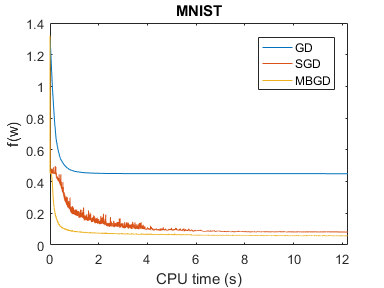
\includegraphics[width=0.6\linewidth]{../../Desktop/Figures/MNIST_SMBGDGD.png}
		\caption{Training an ff-ANN to predict MNIST using \textbf{SGD}, \textbf{MBGD} and \textbf{GD} for comparison. }
		\label{figure:SMBGDGD}
	\end{figure}
	
	\begin{algorithm}
		\caption{Adaptive Trust Region Reduction Schedule (ATRRS)}
		\begin{algorithmic}[1]
			\Function{$\gamma = $ updateGamma($a$, $k$, $e_{c}$, $e_{c-1}$ and $\gamma$)}{}
			%\State{$\gamma = $ updateGamma($a$, $r$, $e^{*}_{a}$, $e_{a}$ and $\gamma$)}		
			\If{$k$ mod $a == 0$}
			\If{$e_{c} > e_{c-1} + tol$}
			\State $\gamma \gets \gamma / 2$
			\Else
			\State do nothing
			\EndIf
			\Else
			\State do nothing
			\EndIf
			\EndFunction
		\end{algorithmic}	
		\label{algorithm:assrs-simple}	
	\end{algorithm}
	
	A learning rate schedule that is often used in practice for stochastic gradient methods is to half the learning rate when progress slows averaging over an epoch \cite{tutorial}. We use a trust region update schedule for our stochastic trust region methods inspired by this learning rate schedule. This schedule is shown in Algorithm \ref{algorithm:assrs-simple}, where $a$ is a block size, $k$ is the number of steps taken so far and the value computed as:
	\begin{equation}
	e_{c} = \frac{1}{a}\sum_{k = a(c-1) + 1}^{ac}{f^{m}(\mathbf{w}_{k})},
	\end{equation}
	where $e_{c}$ is the average gradient during $c^{th}$ epoch and
	\begin{equation}
	c = \left \lfloor{k/a}\right \rfloor.
	\end{equation}
	Recall that $\gamma$ is the trust region size, or ``step size" in the context of adjusted trust region methods.
	 We refer to this schedule we use as the adaptive trust region reduction schedule (ATRRS) and compute only the $\mathbf{p}_{1}$ step from (\ref{equation:p1}). This schedule takes into account the average approximated objective function over a set number of iterations, which we refer to as a \textbf{block}, that has number of iterations $a$. For our experiments we define $a$ to be:
	\begin{equation}
	a = \text{min}(\frac{m}{b_{m}^{small}}, b_{m}^{large}),
	\end{equation}
	where $b_{m}^{small}$ is the value of $b_{m}$ for \textbf{MBTRM} and $b_{m}^{large}$ is approximately the number of training samples that can adequately represent the dataset in order to run \textbf{TRM} which is $b_{m}$ for \textbf{BTRM}. The parameters $b_{m}^{small}$ and $b_{m}^{large}$, known as hyperparameters, are chosen for our experiments using an hyperparameter protocol defined in Appendix \ref{appendix:hyperparameters}, which is run previous to training. This choice of iteration span is to either wait until $m$ training samples have been considered (with possible overlap), or consider a \textbf{block} of $b_{m}^{large}$ iterations which is not dependent on the dataset size itself but rather the characteristics of the data. This means that in cases where $b_{m}$ is small, $b_{m}^{large}$ is used as an upper bound for how often to check progress of the stochastic method. It can also be used for stochastic trust region implementations in online learning contexts where the total training set size is not set.
	
	Since these methods use a small value of $b_{m}$ the computation of $\mathbf{p}_{1}$ is faster using the ``Pearlmutter Trick" each time the product $\mathbf{H}_{k}\mathbf{v}$ must be computed for some vector $\mathbf{v}$ it will take $O(b_{m}n)$ computations rather than $O(mn)$.
	
	\section{Weight Subsampling}

	The other dimension which we can reduce, in the hopes of reducing CPU time for training, is the number of parameters $n$, which is the size of $\mathbf{w}_{k}$ for any iteration $k$. In this thesis we refer to weight subsampling as the random selection of indices of $\mathbf{w}_{k}$, which are the variables of the TRS, at iteration $k$, over which to minimize. We define $\mathbf{a}_{k} \in \mathbb{R}^{b_{w}}$, where $b_{w} < n$ is the number of weights in the subset, to be an array that contains the random indices selected for the weight subset at iteration $k$. Considering only the parameters which have indices contained in $\mathbf{a}_{k}$, the corresponding objective function for the approximate TRS (trust region subproblem) is:
	\begin{equation}
	\delta^{w}(\mathbf{p}_{k}^{w}) = (\mathbf{g}_{k}^{w})^{T}\mathbf{p}_{k}^{w} + \frac{1}{2}(\mathbf{p}_{k}^{w})^{T}\mathbf{H}_{k}^{w}\mathbf{p}_{k}^{w}
	\label{equation:w_subset}
	\end{equation}
	where $\mathbf{p}^{w} \in \mathbb{R}^{b_{w}}$, 
	\begin{equation}
	(\mathbf{g}^{w}_{k})_{i} = (\mathbf{g}_{k})_{(\mathbf{a}_{k})_{i}},
	\end{equation}
	and
	\begin{equation}
	(\mathbf{H}^{w}_{k})_{ij} = (\mathbf{H}_{k})_{(\mathbf{a}_{k})_{i}(\mathbf{a}_{k})_{j}}.
	\end{equation}
	
	In our investigation we want to see how weight subsampling affects the behaviour of the $\mathbf{TRM}$, therefore we implement an algorithm called the trust region method with weight subsampling, \textbf{TRMWS}, which follows Algorithm \ref{algorithm:trs} with the following changes. At the beginning of each iteration a new set of weight indices, $\mathbf{a}_{k}$, are randomly chosen and throughout the iteration, the weight subset version of the gradient, $\mathbf{g}_{k}^{w}$ and that of the Hessian $\mathbf{H}_{k}^{w}$ is used in the place of the full gradient and Hessian at that iteration, $\mathbf{g}_{k}$ and $\mathbf{H}_{k}$ respectively. This means that the variables whose indices are not present in $\mathbf{a}_{k}$ are not updated in iteration $k$.
	
	We also wish to study the effect of weight subsampling on stochastic variations of $\mathbf{TRM}$ that already incorporate SSTS, therefore, we implemented three methods: stochastic trust region method with weight subsampling, $\mathbf{STRMWS}$, mini-batch trust region method with weight subsampling, $\mathbf{MBTRMWS}$, and batch trust region method with weight subsampling, $\mathbf{BTRMWS}$, which are all extensions of methods from the previous section with the addition of weight subsampling.

	
	\section{Hybrid Approach}
	
	The final approach we consider is a hybrid method combining mini-batch gradient descent, $\textbf{MBGD}$, and $\textbf{TRM}$ in order to retain the speed benefit generally seen with $\mathbf{MBGD}$, a well known approach to training ff-ANNs, while decreasing the objective function value using a $\textbf{TRM}$ step occasionally. Note that for the experiments in this thesis the implementation of \textbf{MBGD} and stochasti gradient descent, \textbf{SGD}, updates the learning rate using Algorithm \ref{algorithm:assrs-simple} where trust region size, $\gamma$, is replaced by learning rate, $\eta$, for the stochastic-type gradient method \ref{equation:sgd_update}. 
	
	\begin{algorithm}
		\caption{\textbf{MBGD} $\eta$ Update and \textbf{TRM} Step Incorporation}
		\begin{algorithmic}[1]
			\Function{$\eta = $ checkProgress($a$, $k$, $e_{c}$, $e_{c-1}$ and $\eta$)}{}		
			\If{$r$ mod $a == 0$}
			\If{$e_{c} > e_{c-1} + tol$}
			\State $\eta \gets \eta / 2$
			\State [Take one \textbf{TRM} step with $\gamma = \eta$]
			\Else
			\State do nothing
			\EndIf
			\Else
			\State do nothing
			\EndIf
			\EndFunction
		\end{algorithmic}	
		\label{algorithm:TRMMBGD}	
	\end{algorithm}
	
	Our hybrid approach, which we refer to as \textbf{TRMMBGD}, is to follow $\mathbf{MBGD}$ but each time the learning rate is halved due to a lack of progress between iteration blocks, the learning algorithm solves the TRS for the next step rather than using the approximate gradient step and then returns to $\mathbf{MBGD}$ on the following iteration. This is shown in Algorithm \ref{algorithm:TRMMBGD}. By using a TRS step only when we are not seeing progress in reducing the objective function with \textbf{MBGD}, we hope to benefit heavily from the fast first order decent by $\mathbf{MBGD}$ and reserve solving the TRS for when it would be most beneficial.
	
	\section{Full Hessian vs Hessian Free}
	
	Our methods can all be performed using either a function which computes the product $\mathbf{H}_{k}\mathbf{v}$ for any given vector $\mathbf{v}$, or by using the full Hessian $\mathbf{H}_{k}$ which must be computed first. When using a Hessian free approach, the ``Pearlmutter Trick" (see Appendix \ref{appendix:pearlmutter}) must be performed each time $\mathbf{H}_{k}\mathbf{v}$ is computed for some vector $\mathbf{v}$. This takes $O(mn)$ computations where $m$ is the number of training samples and $n$ is the number of parameters. Computing $\mathbf{H}_{k}\mathbf{v}$ when we compute $\mathbf{H}_{k}$ only takes $O(n^{2})$ and often $n < m$. This, however, requires the added cost of computing $\mathbf{H}_{k}$. We simplified this discussion by using symbols $n$, $m$, and $\mathbf{H}_{k}$ which are the symbols relevant to the $\mathbf{TRM}$. This discussion is also true for $b_{w}$, any value of $b_{m}$ and the approximate or lower dimension Hessian matrix being used. It is therefore relevant to all method variations presented in this chapter.
	
	In order to decide for which methods we compute the full Hessian matrix and for which we did not, we timed the first 1000 iterations (or fewer for those that converged prior to 1000 iterations) of all methods on all datasets using both approaches. These results are presented in Appendix \ref{appendix:fhhf}.  We chose to keep the Hessian computation approach for each method consistent across datasets for our experimental results. If a method computed each step taking on average less CPU time using the Hessian free approach for the majority of datasets, the Hessian free approach was used for all datasets in experimentation and otherwise the full Hessian approach was used. We show the resulting choice of Hessian computation in Table \ref{table:FHHF}. 
	
	
	\begin{table}[h]
		\begin{center}
			\begin{tabular}{ |c|c| }  
				\hline
				\textbf{Method} & \textbf{Hessian Computation Approach}  \\
				\hline 
				\textbf{TRM} & FH\\
				\textbf{TRMWS} & FH\\
				\textbf{BTRM} & \textbf{HF}\\
				\textbf{BTRMWS} & FH \\
				\textbf{MBTRM} & \textbf{HF} \\ 
				\textbf{MBTRMWS} & FH \\
				\textbf{STRM} &\textbf{HF} \\
				\textbf{STRMWS} & FH \\
				\textbf{TRMMBGD} &\textbf{HF} \\
				\hline
			\end{tabular}
			\caption{The approach used for computing Hessian information in each method. HF refers to ``Hessian Free" and FH refers to ``Full Hessian". HF is in bold to more easily distinguish between the two values. }
			\label{table:FHHF}
		\end{center}
	\end{table}
	
	
	\section{Summary}
	
	Descriptions of labels for the methods used in this investigation are presented in Table \ref{table:algorithms}, which use the definitions of weight subsampling and stochastic subsampling of training samples (SSTS) from this chapter. These methods cover a broad range of approaches to reduce the computations required for a step of the base method, $\mathbf{TRM}$. The method of choosing hyperparameters ($b_{w}$, $b_{m}^{large}$, $b_{m}^{small}$ etc) is defined in Appendix \ref{appendix:hyperparameters}.
	
	\begin{table}[h]
		\begin{center}
			\begin{tabular}{ |c|l| }  
				\hline
				\textbf{Label} & \textbf{Method definition / description}  \\
				\hline
				\textbf{TRM} &  standard trust region method, Algorithm \ref{trust region method}. \\
				\textbf{TRMWS} & \textbf{TRM} with weight subsampling. \\
				\textbf{BTRM} & \textbf{TRM} with SSTS.\\
				\textbf{BTRMWS} & \textbf{TRM} with SSTS and weight subsampling.  \\
				\textbf{MBTRM} & \textbf{TRM} with SSTS, using only the $\mathbf{p}_{1}$ step and \\ &
				the adaptive trust region reduction schedule (ATRRS), Algorithm \ref{algorithm:assrs-simple}. \\ 
				\textbf{MBTRMWS} & \textbf{MBTRM} with weight subsampling as well. \\
				\textbf{STRM} & special case of \textbf{MBTRM} where $b_{m} = 1$. \\
				\textbf{STRMWS} & special case of \textbf{MBTRMWS} where $b_{m} = 1$. \\
				\textbf{MBGD} & Mini-batch gradient descent with learning rate updated using the \\ & Algorithm \ref{algorithm:assrs-simple}  after replacing $\gamma$ by the learning rate.\\
				\textbf{SGD} & \textbf{MBGD} with $b_{m} = 1$. \\
				\textbf{TRMMBGD} & \textbf{MBGD} where \textbf{TRM} step is used when \textbf{MBGD}'s progression slows. \\
				\hline
			\end{tabular}
			\caption{Training algorithm definitions used for numerical exploration, and their labels, which will be used to reference them.}
			\label{table:algorithms}
		\end{center}
	\end{table}
	
	
	\chapter{Numerical Results}
	
	
	In this chapter we present the results from a large array of experiments. We compare methods, defined in Table \ref{table:algorithms}, performed on various datasets in order to gain insight into their behaviour when used for training ff-ANNs. 
	
	
	\section{Experimental Set-up}
	
	The algorithms presented in Chapter 4 are implemented in MATLAB and available at  https://github.com/cwkinros/Stochastic\_TRM\_Exploration. Experiments were run on individual nodes of the University of Waterloo Chardonnay cluster consisting of 8 nodes. Each of these nodes have 2x Intel E5-2671 (8C) CPUs, 128 GB of memory and 15T LSI SAS2308 of disk space. The nodes run Linux and the specific experiments are run in the 64-bit R2013b version of MATLAB on these machines.
	
	\subsection{Datasets}
	
	Sizes of datasets are displayed in Table \ref{table:datasets}. The datasets were chosen to have a variety of sizes in terms of the number of independent variables, $n_{0}$, and the number of classes, both which affect the number of parameters, $n$, in the resulting ff-ANN. They also have differing numbers of training examples, $m$. They cover a few application domains as shown in Table \ref{table:datasettopics}, and are expected to have different properties. For instance, most datasets have separable classes, except Habe where the class label appears virtually unrelated to the independent variables as can be seen in Figure \ref{figure:haberman}.
	
	\begin{table}[h]
		\begin{center}
			\begin{tabular}{ |c|c|c|c|c| }  
				\hline
				\textbf{label} & \textbf{$m$} & \textbf{$n_{0}$} & \textbf{\# classes} & $n$  \\
				\hline
				MNIST & 60000 & 100 & 10 & 1120 \\
				Derm & 366 & 33 & 6 & 406 \\
				IRIS & 150 & 4 & 3 & 83\\
				Nurs & 12960 & 8 & 5 & 145 \\
				Habe & 306 & 3 & 2* & 51 \\ 
				\hline
			\end{tabular}
			\caption{Datasets used for experimentation. *Habe uses a single dependent variable with two states, each to represent one of the classes.}
			\label{table:datasets}
		\end{center}
	\end{table}
	
	\begin{table}[h]
		\begin{center}
			\begin{tabular}{ |c|l|c| }  
				\hline
				\textbf{label} & \textbf{Description} & \textbf{Source}\\
				\hline
				MNIST & handwritten digits & \cite{mnist}\\
				\hline
				Derm & differential diagnosis of erythemato-squamous diseases & \cite{Derm}\\
				\hline
				IRIS & predict class of iris plant & \cite{IRIS}\\
				\hline
				Nurs & rank applications to nursery schools & \cite{Nurs}\\
				\hline
				Habe & predict survival status for patients with breast cancer  & \cite{Habe}\\ 
				\hline
			\end{tabular}
		\end{center}
		\caption{Datasets used for experimentation.}
		\label{table:datasettopics}
		%\end{center}
	\end{table}
	
	\begin{figure}[h]
		\centering
		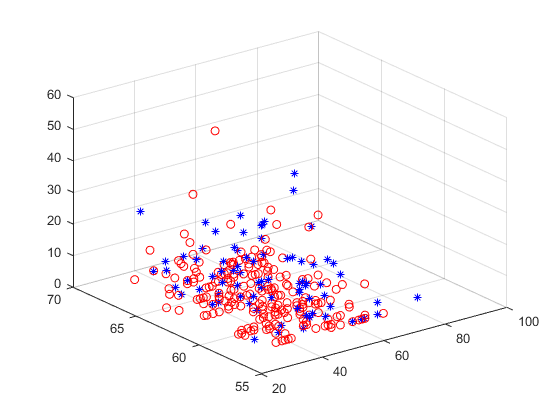
\includegraphics[width=0.5\linewidth]{../../Desktop/figures/haberman_data.png}
		\caption{Visualization of Habe dataset where classes are represented by shape and colour. This shows the difficulty in learning this dataset, there is no clear separation between classes.}
		\label{figure:haberman}
	\end{figure}
	
	
	\subsection{Network Structure}
	
	The networks used for experimentation are two-layer, fully connected ff-ANNs. The activation function used is the sigmoid function, both at the hidden layer and at the final layer:
	
	\begin{equation}
	\sigma_{1}(x) = \sigma_{2}(x) = \frac{1}{1 - e^{-x}}.
	\end{equation}
	
	An example of the network structure, applied to the Derm dataset, is shown in Figure \ref{figure:structure}. The value for $n_{0}$ depends on the dataset, and can be seen in Table \ref{table:datasets}, and $n_{2}$ is the number of classes in the networks shown in Table
	\ref{table:datasets} for our experiments, with the exception of the Habe dataset where we use $n_{2} = 1$ for a two class problem. All networks for the five datasets in Table \ref{table:datasets} contain 10 hidden units. 
	
	
	\begin{figure}[h]
		\centering
		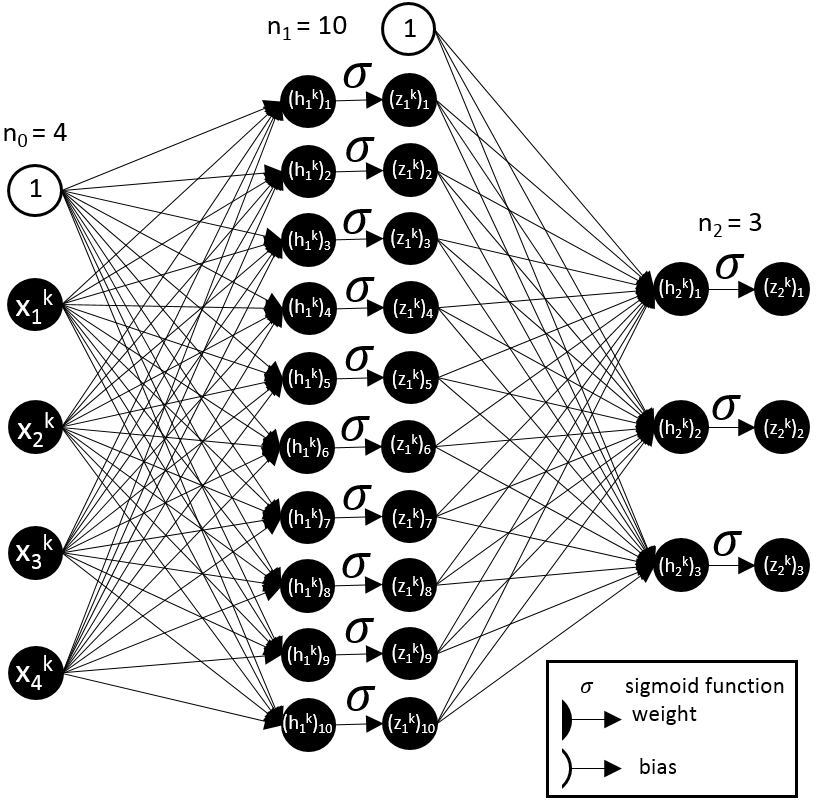
\includegraphics[width=1.0\linewidth]{../../Desktop/figures/structure.PNG}
		\caption{Structure of ff-ANN for learning the Derm dataset. Used as visual example to show resulting structure for a given $n_{0}$ and $n_{2}$ which are based on the dataset.}
		\label{figure:structure}
	\end{figure}

	
	\section{Methods for Comparison}
	
	In this section we define criteria we use for ranking optimization curves, the curve representing the objective function value over time, while undergoing an iterative optimization method. It can be difficult to make comparisons between two different optimization curves that display different behaviours. In order to be specific in our analysis of optimization algorithms we define a ranking method. To begin, we first present the two possible comparison approaches include:
	\begin{enumerate}
		\item CPU time taken to reach a specific objective function value.
		\item Objective function value achieved within a certain time.
	\end{enumerate}
	
	Both of these metric comparisons involve choosing either a specific objective function value or time to set as a fixed value and then compare using the other metric. The final measurement can depend on this choice, making it critical that there is an objective procedure used to make the choice. We will analyze the majority of the experimental results using the metric defined in the following section, which uses the data to define an objective function value for CPU time measurements. Simpler comparison methods will be explained when they are used.
	
	\subsection{Time Required for a Reasonable Solution}
	
	The main comparison method we use in our numerical investigation is what we refer to as time required for a reasonable solution (TRRS). This follows the first metric concept where we compare the CPU time taken to reach a specific objective function value. The specific objective function value used is dependent on the methods being compared which means that the TRRS can only be used to compare two methods, otherwise this objective function may differ and change the result. 
	
	Before we define TRRS, we will first introduce a few notations. Suppose $K_{a}$ and $K_{b}$ are the final iteration numbers for method $a$ and $b$, respectively. Let $cpu(K_{a})$ ($cpu(K_{b})$) be the CPU time taken for performing $K_{a}$ ($K_{b}$) iterations by method $a$ (method $b$). For the purpose of comparison, we will fix the time for both methods and the fixed time is chosen to be the minimum of the two:
	\begin{equation}
	T = min(cpu(K_{a}), cpu(K_{b})).
	\end{equation}
	
	Accordingly, let $K_{T}^{a}$ ($K_{T}^{b}$) be the smallest iteration number for method $a$ (method $b$) such that $cpu(K_{T}^{a}) >= T$ $(cpu(K_{T}^{b}) >= T)$. 
	
	We then consider the values of the objective function for all iterates generated by the two methods and find the minimum one. More precisely, we define:
	\begin{equation}
	\kappa = min(f(\mathbf{w}_{k_{a}}^a), f(\mathbf{w}_{k_{b}}^b))       \quad k_{a} = 0, 1, ..., K_{T}^{a}, \  k_{b} = 0, 1, ..., K_{T}^{b}
	\end{equation}
	where $\mathbf{w}_{k_{a}}^{a}$ and $\mathbf{w}_{k_{b}}^{b}$ are the approximate solutions generated by method $a$ and method $b$, respectively.
	
	Now we call a solution, $\mathbf{w}_{k}$, a reasonable solution if $f(\mathbf{w}_{k})$ is close to k. Specifically,
	\begin{equation}
	f(\mathbf{w}_{k}) <= \psi,
	\end{equation}
	where
	\begin{equation}
	\psi = k + \Delta |f(\mathbf{w}_0) - k|.
	\end{equation}	
	Here $\mathbf{w}_{0}$ is the vector of initial parameters and $\Delta$ is given by the user.
	
	Finally, TRRS for method $a$ is defined to be $cpu(K_{a}^{\psi})$ where $K_{a}^{\psi}$ is the first iteration such that $\mathbf{w}_{K_{a}^{\psi}}^a$ is considered a reasonable solution. TRRS for method $b$ is defined similarly.
		
	\section{CPU time of TRM vs SGD}
	
	The first question we wanted to answer in this investigation is simply: How much slower is the \textbf{TRM} compared to \textbf{SGD}. We run \textbf{SGD} to train each dataset in Table \ref{table:datasettopics}. At this point we search for the smallest objective function value achieved during \textbf{SGD} training and define our CPU time metric to be when the CPU time at the first iteration that a method reaches within 1\% (based on the initial objective function) of the smallest objective function value achieved by \textbf{SGD}. The results are presented in Table \ref{t_trm_sgd}. 
	
	These results show that it takes \textbf{TRM} much longer, in terms of CPU time,
	to reach the goal objective function value computed using the \textbf{SGD} results, than \textbf{SGD}. The proportional time discrepancy is particularly large for MNIST and Derm datasets which both have a larger number of parameters. MNIST has by far the largest magnitude increase in time, which makes sense since it has both the largest number of parameter and the largest number of training samples. 
	
	\begin{table}[h] 
		\centering 
		\begin{tabular}{ |c|l|l| } 
			\hline 
			\textbf{Dataset} & CPU time (s) \textbf{TRM} & CPU time (s) \textbf{SGD}\\ 
			\hline 
			Derm &5.0535 & $\mathbf{0.23578}$\\ 
			\hline 
			Habe &0.14527 & $\mathbf{0.092241}$\\ 
			\hline 
			IRIS &0.46323 & $\mathbf{0.18152}$\\ 
			\hline 
			MNIST &2607.145 & $\mathbf{4.2025}$\\ 
			\hline 
			Nurs &39.7811 & $\mathbf{5.3361}$\\ 
			\hline 
		\end{tabular} 
		\caption{Time taken to reach within 1\% of minimum $f(\mathbf{w})$ achieved by \textbf{SGD} for both \textbf{SGD} and \textbf{TRM}.} \label{t_trm_sgd} \end{table}
	
	\section{Using TRM and MBGD in Hybrid: TRMMBGD}
	
	In this section we explore whether we can make an improvement to traditional stochastic gradient methods, specifically \textbf{MBGD}, using the \textbf{TRM} step when necessary. Recall the mechanism for switching between the two described in \S{4.3}, which combines them by prioritizing \textbf{MBGD} and only using \textbf{TRM} when \textbf{MBGD} is not effectively reducing the objective function. 
	
	The results of this experiment are found in Figure \ref{figure:TRMMBGD}. The two methods, \textbf{MBGD} and \textbf{TRMMBGD} perform very similarly at low CPU time with \textbf{MBGD} slightly outperforming \textbf{TRMMBGD} in terms of values of TRRS for $\Delta=5\%$ and $10\%$, shown in Tables \ref{TRMMBGD5} and \ref{TRMMBGD10} respectively.  In all TRRS tables, the faster method based on the $\Delta$ used in each set of results, is in bold. The dash represents when there is no TRRS for a method, which means that the method did not achieve a reasonable solution based on the definition of reasonable in \S{5.2.1}. Looking at values of TRRS for $\Delta=1\%$, shown in Table \ref{TRMMBGD1}, we see that either $\textbf{TRMMBGD}$ performs as well as $\mathbf{MBGD}$, where there is less than a 0.1 second discrepency for the TRRS, or in the case of Habe, IRIS and Nurs, \textbf{TRMMBGD} achieves a better solution overall. The most extreme improvement in objective function value is seen by IRIS in Figure \ref{TRMMBGD1}, where \textbf{TRMMBGD} continues to make significant improvements to the objective function while the objective function being minimized by \textbf{MBGD} has stopped decreasing in magnitude. 
	
	In conclusion, we find that \textbf{TRMMBGD} is an effective improvement over \textbf{MBGD}. In some cases the two methods perform very similarly, whereas for some datasets the optimization curve of \textbf{TRMMBGD} performs similarly early on but achieves a lower final objective function eventually. 
	
	
	\begin{figure}
		\centering
		\begin{subfigure}{.45\textwidth}
			\includegraphics[width=\textwidth]{../../Desktop/Figures/Derm_TRMMBGD23.png}
		\end{subfigure}
		\begin{subfigure}{.45\textwidth}
			\includegraphics[width=\textwidth]{../../Desktop/Figures/IRIS_TRMMBGD23.png}
		\end{subfigure}
		\begin{subfigure}{.45\textwidth}
			\includegraphics[width=\textwidth]{../../Desktop/Figures/Habe_TRMMBGD23.png}
		\end{subfigure}
		\begin{subfigure}{.45\textwidth}
			\includegraphics[width=\textwidth]{../../Desktop/Figures/Nurs_TRMMBGD23.png}
		\end{subfigure}
		\begin{subfigure}{.45\textwidth}
			\includegraphics[width=\textwidth]{../../Desktop/Figures/MNIST_TRMMBGD23.png}
		\end{subfigure}
		\caption{Running TRMMBGD vs MBGD for training ff-ANNs on five datasets.}
		\label{figure:TRMMBGD}
	\end{figure}
	
\begin{table}[h] 
	\centering 
	\begin{tabular}{ |c|l|l| } 
		\hline 
		\textbf{Dataset} & CPU time (s) \textbf{MBGD} & CPU time (s) \textbf{TRMMBGD}\\ 
		\hline 
		Derm & $\mathbf{0.18436}$ &0.23661\\ 
		\hline 
		Habe & - & $\mathbf{1.8206}$\\ 
		\hline 
		IRIS & - & $\mathbf{0.37217}$\\ 
		\hline 
		MNIST &2.096 & $\mathbf{1.925}$\\ 
		\hline 
		Nurs &1.9246 & $\mathbf{1.4415}$\\ 
		\hline 
	\end{tabular} 
	\caption{TRRS results for $\Delta = 1 \%$} \label{TRMMBGD1} \end{table}
	
\begin{table}[h] 
	\centering 
	\begin{tabular}{ |c|l|l| } 
		\hline 
		\textbf{Dataset} & CPU time (s) \textbf{MBGD} & CPU time (s) \textbf{TRMMBGD}\\ 
		\hline 
		Derm & $\mathbf{0.040571}$ &0.044899\\ 
		\hline 
		Habe & $\mathbf{0.35471}$ &0.45047\\ 
		\hline 
		IRIS & - & $\mathbf{0.28553}$\\ 
		\hline 
		MNIST &0.38535 & $\mathbf{0.35748}$\\ 
		\hline 
		Nurs & $\mathbf{0.40615}$ &0.51935\\ 
		\hline 
	\end{tabular} 
	\caption{TRRS results for $\Delta = 5 \%$} \label{TRMMBGD5} \end{table}
	
\begin{table}[h] 
	\centering 
	\begin{tabular}{ |c|l|l| } 
		\hline 
		\textbf{Dataset} & CPU time (s) \textbf{MBGD} & CPU time (s) \textbf{TRMMBGD}\\ 
		\hline 
		Derm &0.026375 & $\mathbf{0.025359}$\\ 
		\hline 
		Habe &0.16741 & $\mathbf{0.15084}$\\ 
		\hline 
		IRIS & - & $\mathbf{0.23544}$\\ 
		\hline 
		MNIST &0.22061 & $\mathbf{0.19866}$\\ 
		\hline 
		Nurs &0.23353 & $\mathbf{0.21426}$\\ 
		\hline 
	\end{tabular} 
	\caption{TRRS results for $\Delta = 10 \%$} \label{TRMMBGD10} \end{table}
	
	\section{Stochastic TRMs}
	
	We devote this section to evaluating whether or not stochastic subsampling improves the performance of $\mathbf{TRM}$ in terms of the TRRS measure, from \S{5.2.1}, for either of the trust region size update schemes discussed in Chapter 4. We also present figures of the methods' progress over time, as we have done in the previous section, to provide insight into their behaviour.
	
	\subsection{Adaptive Trust Region Reduction Scheme}
	
	In this section we study the effectiveness of applying stochastic sampling methods, used with the adaptive trust region reduction scheme (ATRRS) in Algorithm \ref{algorithm:assrs-simple}, to $\mathbf{TRM}$. We want to measure TRRS for $\mathbf{TRM}$ and its variatons based on stochastic sampling, $\mathbf{MBTRM}$ and $\mathbf{STRM}$, in order to determine if stochastic sampling variations are an effective way to speed up the $\mathbf{TRM}$ method on ff-ANN when paired with the adaptive trust region reduction scheme. 

	We set up an experiment to determine whether or not stochastic subsampling of training examples is an effective method for speeding up $\mathbf{TRM}$. The experiment involves running $\mathbf{TRM}$, $\mathbf{STRM}$ and $\mathbf{MBTRM}$ on the five datasets listed in Table \ref{table:datasets} and recording CPU time and the true objective function, $f(\mathbf{w}_{k})$, at each iteration $k$. The results of this experiment are displayed in Figure \ref{figure:SMBTRMTRM}. Results in Figure \ref{figure:SMBTRMTRM} are cutoff on the x-axis at the minimum total CPU time between all three methods, based on the protocol for measuring TRRS. These graphs show significant differences in the objective function values at any time between \textbf{MBTRM} and \textbf{STRM} that are not seen between $\mathbf{SGD}$ and $\mathbf{MBGD}$. Specifically, $\mathbf{MBTRM}$ seems to reduce the objective function in all cases, despite sometimes not doing as well as \textbf{TRM}. On the other hand, in the case of the Derm dataset, \textbf{STRM} does not even decrease the objective function from the initial value. 
	
	\begin{figure}
		\centering
		\begin{subfigure}{.45\textwidth}
			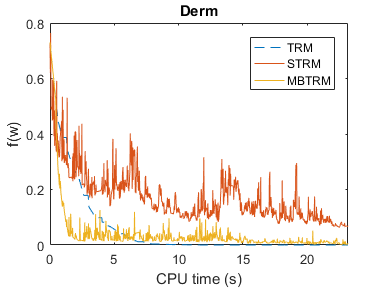
\includegraphics[width=\textwidth]{../../Desktop/Figures/Derm_SMBTRMTRM.png}
		\end{subfigure}%
		\begin{subfigure}{.45\textwidth}
			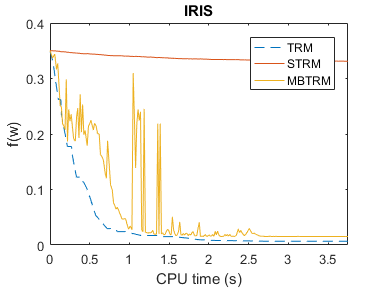
\includegraphics[width=\textwidth]{../../Desktop/Figures/IRIS_SMBTRMTRM.png}
		\end{subfigure}
		\begin{subfigure}{.45\textwidth}
			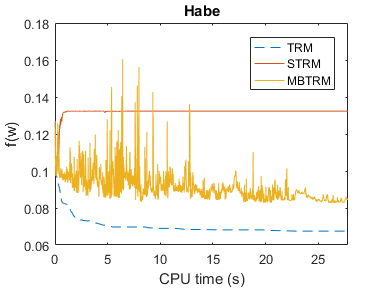
\includegraphics[width=\textwidth]{../../Desktop/Figures/Habe_SMBTRMTRM.png}
		\end{subfigure}
		\begin{subfigure}{.45\textwidth}
			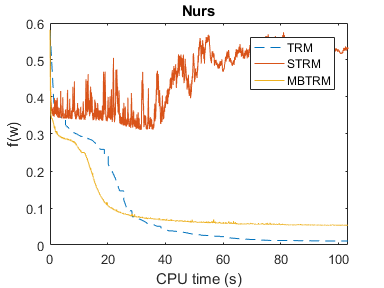
\includegraphics[width=\textwidth]{../../Desktop/Figures/Nurs_SMBTRMTRM.png}
		\end{subfigure}
		\begin{subfigure}{.45\textwidth}
			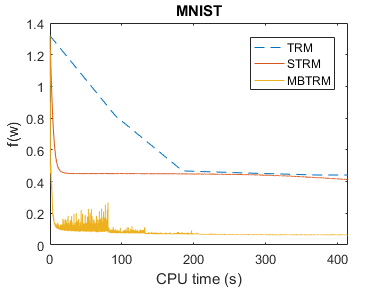
\includegraphics[width=\textwidth]{../../Desktop/Figures/MNIST_SMBTRMTRM.png}
		\end{subfigure}
		\caption{Comparing \textbf{TRM} with stochastic training example subsampling \textbf{TRM} methods (\textbf{STRM} and \textbf{MBTRM}), based on objective function, $f(\mathbf{w})$, vs CPU time.}
		\label{figure:SMBTRMTRM}
	\end{figure}
	
	
	We use TRRS to quantitatively evaluate \textbf{MBTRM} and \textbf{STRM} as potential faster variations of \textbf{TRM}. We measure the time required to obtain a reasonable solution (TRRS) where $\Delta = 1\%$, $5\%$, $10\%$. We compare both \textbf{MBTRM} and \textbf{STRM} against $\mathbf{TRM}$, and the results are displayed in Tables \ref{SMBTRMTRM1}, \ref{SMBTRMTRM5}, and \ref{SMBTRMTRM10} respectively. Recall that TRRS is a measure between two methods only, therefore we compare \textbf{MBTRM} to \textbf{TRM} and \textbf{STRM} to \textbf{TRM} separately. In each table (\ref{SMBTRMTRM1}, \ref{SMBTRMTRM5}, \ref{SMBTRMTRM10}) columns 2 and 3 contain the results from measuring TRRS for \textbf{TRM} and \textbf{MBTRM} and columns 4 and 5 show the results from measuring TRRS for \textbf{TRM} and \textbf{STRM}.
	
	We find that \textbf{TRM} has a lower TRRS than \textbf{STRM} for all training runs, except for in the case of MNIST where \textbf{STRM} gets to $\Delta = 10\%$ faster than $\textbf{TRM}$. Once we decrease $\Delta$ to $5\%$ and $1\%$, \textbf{TRM} outperforms \textbf{STRM}. This indicates that generally, \textbf{STRM} as a variation of \textbf{TRM}, is not an effective speed up approach compared to the performance of the original \textbf{TRM} method.
	
	Results were found to be more mixed when we compare TRRS between \textbf{MBTRM} and \textbf{TRM}. We find that for $\Delta = 5\%$ and $10\%$ \textbf{MBTRM} actually achieves a faster TRRS than \textbf{TRM} on MNIST and Derm datasets. This is somewhat unexpected since Nurs has a larger number of training samples than Derm and therefore would appear to be a better candidate for a mini-batch method. 
	
	Recall from \S4.4 that the algorithms \textbf{MBTRM} and \textbf{STRM} both use the Hessian Free approach where the `Pearlmutter Trick' is called with $O(nb_{m})$ time complexity each time we compute the product $\mathbf{H}_{k}\mathbf{v}$ for any $\mathbf{v} \in \mathbb{R}^{n}$ where $\mathbf{H}_{k}$ is the Hessian of the objective function at iteration $k$. This is in contrast to the method in $\mathbf{TRM}$ where we compute the Hessian matrix fully before solving for $\mathbf{p}_{1}$ and $\mathbf{p}_{0}$. 
	
	Finally, we note that \textbf{MBTRM} has a lower TRRS when used to train using the MNIST dataset, even for the case when $\Delta = 1\%$. In conclusion, for some datasets we find that \textbf{MBTRM} can improve upon \textbf{TRM} however it is not a consistent trend across a diverse range of datasets.
	
	\begin{table}[h] 
		\centering 
		\begin{tabular}{ |c||l|l||l|l||l|l| } 
			\hline 
			\textbf{Dataset} & \textbf{TRM} & \textbf{MBTRM} & \textbf{TRM} & \textbf{STRM} & \textbf{TRM} & \textbf{BTRM} \\ 
			\hline 
			\hline 
			Derm & $\mathbf{7.3726}$ &14.8783 & $\mathbf{7.3726}$ & - &7.3726 & $\mathbf{2.827}$\\ 
			\hline 
			Habe & $\mathbf{15.8215}$ & - & $\mathbf{11.8777}$ & - & $\mathbf{21.0525}$ & -\\ 
			\hline 
			IRIS & $\mathbf{1.8912}$ & - & $\mathbf{1.8912}$ & - & $\mathbf{1.8912}$ & -\\ 
			\hline 
			MNIST & - & $\mathbf{83.7168}$ & $\mathbf{1574.484}$ & - & - & $\mathbf{1799.908}$\\ 
			\hline 
			Nurs & $\mathbf{67.7825}$ & - & $\mathbf{67.7825}$ & - & $\mathbf{67.7825}$ & -\\ 
			\hline 
		\end{tabular} 
		\caption{TRRS results for $\Delta = 1 \%$} \label{SMBTRMTRM1}  \end{table}
	
\begin{table}[h] 
	\centering 
	\begin{tabular}{ |c||l|l||l|l||l|l| } 
		\hline 
		\textbf{Dataset} & \textbf{TRM} & \textbf{MBTRM} & \textbf{TRM} & \textbf{STRM} & \textbf{TRM} & \textbf{BTRM} \\ 
		\hline 
		\hline 
		Derm &5.8078 & $\mathbf{1.455}$ & $\mathbf{5.8078}$ & - &5.8078 & $\mathbf{1.383}$\\ 
		\hline 
		Habe & $\mathbf{2.652}$ & - & $\mathbf{2.3852}$ & - & $\mathbf{3.477}$ & -\\ 
		\hline 
		IRIS & $\mathbf{0.84902}$ &1.1691 & $\mathbf{1.0384}$ & - & $\mathbf{1.0384}$ &1.8596\\ 
		\hline 
		MNIST & - & $\mathbf{6.4677}$ & $\mathbf{1389.245}$ & - & - & $\mathbf{146.8234}$\\ 
		\hline 
		Nurs & $\mathbf{41.1667}$ & - & $\mathbf{41.1667}$ & - &41.1667 & $\mathbf{32.9154}$\\ 
		\hline 
	\end{tabular} 
	\caption{TRRS results for $\Delta = 5 \%$} \label{SMBTRMTRM5} \end{table}
	
\begin{table}[h] 
	\centering 
	\begin{tabular}{ |c||l|l||l|l||l|l| } 
		\hline 
		\textbf{Dataset} & \textbf{TRM} & \textbf{MBTRM} & \textbf{TRM} & \textbf{STRM} & \textbf{TRM} & \textbf{BTRM} \\ 
		\hline 
		\hline 
		Derm &4.4035 & $\mathbf{1.2892}$ & $\mathbf{4.4035}$ &20.9612 &4.4035 & $\mathbf{1.024}$\\ 
		\hline 
		Habe & $\mathbf{1.3666}$ & - & $\mathbf{1.3274}$ & - & $\mathbf{1.4662}$ & -\\ 
		\hline 
		IRIS & $\mathbf{0.71805}$ &0.97309 & $\mathbf{0.71805}$ & - & $\mathbf{0.71805}$ &1.3308\\ 
		\hline 
		MNIST & - & $\mathbf{3.932}$ &1111.175 & $\mathbf{605.5431}$ & - & $\mathbf{9.3117}$\\ 
		\hline 
		Nurs & $\mathbf{32.7128}$ &37.7004 & $\mathbf{32.7128}$ & - &32.7128 & $\mathbf{11.8563}$\\ 
		\hline 
	\end{tabular} 
	\caption{TRRS results for $\Delta = 10 \%$} \label{SMBTRMTRM10} \end{table}
	
	\subsection{Traditional TRM $\gamma$ Update Scheme}
	
	We train the same networks using \textbf{BTRM} and \textbf{TRM} in order to test whether using stochastic sampling of training examples on the full \textbf{TRM} method, including the traditional \textbf{TRM} update scheme, is an effective method for improving $\mathbf{TRM}$ performance in terms of TRRS. The batch size is chosen using the hyperparameter value search scheme (see Appendix \ref{appendix:hyperparameters}). The hyperparameter which defined the batch size is $b_{m}^{large}$. The value of $b_{m}^{large}$ is greater than that of $b_{m}^{small}$ for all datasets, which is why we use the label ``large". We expect that a greater batch size will mean that the approximation of the trust region subproblem more closely resembles the actual subproblem. Therefore, we expect that the use of the traditional trust region size update in Algorithm \ref{trust region size} will be effective at predicting what size of region can be accurately modeled using the previous step accuracy.
	
	The optimization curves produced by running this experiment on each dataset, are presented in Figure \ref{figure:BTRMTRM}. Visually, we can see that the \textbf{BTRM} curves start out faster than \textbf{TRM} for training most datasets besides Iris, where the speed is similar, and Habe, where \textbf{BTRM} is found to be essentially ineffective at minimizing the objective function. This result for Habe is expected for any stochastic method since subsets are not sufficiently representative of the full set as we discovered in Figure \ref{figure:haberman}. The low signal to noise ratio means that it is possible that the noise of the stochastic approximation has more effect on the step choice than the underlying signal we wish to learn.
	
	 We can see the quantitative TRRS measurements in Tables \ref{SMBTRMTRM1}, \ref{SMBTRMTRM5} and \ref{SMBTRMTRM10} in columns 6 and 7. In the results for the MNIST and Derm datasets we see that for all values of $\Delta$, \textbf{BTRM} outperforms \textbf{TRM} in terms of TRRS. On the Nurs dataset we see that for $\Delta = 5\%$ and $10\%$ \textbf{BTRM} reaches a reasonable solution faster than \textbf{TRM} but does not reach within $1\%$ of the final solution for the \textbf{TRM}. This means that \textbf{BTRM} successfully speeds up \textbf{TRM} for training Nurs, but it is at the expense of the quality of final solution. For IRIS the results are slightly worse when trained with \textbf{BTRM} compared to \textbf{TRM}, but reasonably similar. Training using the Habe dataset resulted in no cases where \textbf{BTRM} outperforms \textbf{TRM} which we have discussed during the discussion of Figure \ref{figure:BTRMTRM}.
	 
	We conclude that \textbf{BTRM} can decrease the TRRS compared to \textbf{TRM} for training ff-ANNs on datasets where the signal to noise ratio is high. We hypothesize that stochastic methods perform poorly since the poor signal to noise ratio means that the direction of each stochastic step may be more influenced by the noise of the small subset of samples rather than the underlying trend. To understand this more clearly, imagine performing a linear regression problem on a dataset with a very small signal to noise ratio. With 1000 samples, the signal may be picked up but with only 2 the predicted linear relationship will be heavily influenced by noise effecting the two points. 
	
	\begin{figure}
		\centering
		\begin{subfigure}{.45\textwidth}
			\includegraphics[width=\textwidth]{../../Desktop/figures/Derm_BTRMTRM3.png}
		\end{subfigure}%
		\begin{subfigure}{.45\textwidth}
			\includegraphics[width=\textwidth]{../../Desktop/figures/IRIS_BTRMTRM3.png}
		\end{subfigure}
		\begin{subfigure}{.45\textwidth}
			\includegraphics[width=\textwidth]{../../Desktop/figures/Habe_BTRMTRM3.png}
		\end{subfigure}
		\begin{subfigure}{.45\textwidth}
			\includegraphics[width=\textwidth]{../../Desktop/figures/Nurs_BTRMTRM3.png}
		\end{subfigure}
		\begin{subfigure}{.45\textwidth}
			\includegraphics[width=\textwidth]{../../Desktop/figures/MNIST_BTRMTRM3.png}
		\end{subfigure}
		\caption{Comparing \textbf{TRM} with stochastic training example subsampling \textbf{TRM} method, \textbf{BTRM}, based on objective function over CPU time.}
		\label{figure:BTRMTRM}
	\end{figure}

	
	\section{Reducing the Dimentionality of TRS}
	
	We experiment with weight subsampling added to the \textbf{TRM} algorithm to train ff-ANNs using the five datasets with both \textbf{TRMWS} and \textbf{TRM} and comparing the results. The results of these experiments are shown in Figure \ref{figure:TRMWS}. Specifically, we plot the objective function vs the CPU time as we have done for stochastic methods in the previous sections. In terms of the qualitative behaviour we can see that for datasets Derm, IRIS and MNIST, this method is beneficial. For Habe, weight subsampling actually slows down the overall progress initially but it eventually surpases \textbf{TRM} in objective function over CPU time. 
	
	In order to compare these methods quantitatively, we display the TRRS in Tables \ref{table:TRMWS1}, \ref{table:TRMWS5} and \ref{table:TRMWS10} for the TRRS parameter $\Delta = 1\%$, $5\%$ and $10\%$ respectively. We observe improvement in terms of TRRS for training ff-ANNs on Derm, IRIS and MNIST for all values of $\Delta$ when adding weight subsampling to \textbf{TRM}. For Nurs we see that \textbf{TRM} has a shorter TRRS for all values of $\Delta$ displayed, however we note in Figure \ref{figure:TRMWS} that Nurs is faster at getting a very approximate solution and is passed before the $\Delta=10\%$ mark. Finally, we see that \textbf{TRMWS} outperforms \textbf{TRM} on the Habe dataset for only the lowest value of $\Delta$. These are mixed results, but we observe that \textbf{TRMWS} is faster at the beginning of training for $80\%$ of our datasets, and has a better TRRS for $\Delta=1\%$ on $80\%$ datasets as well. Therefore we can conclude that the variation, \textbf{TRMWS}, improves \textbf{TRM} in many cases.
	
\begin{table}[h] 
	\centering 
	\begin{tabular}{ |c||l|l||l|l|| } 
		\hline 
		\textbf{Dataset} & \textbf{TRM} & \textbf{TRMWS} & \textbf{BTRM} & \textbf{BTRMWS} \\ 
		\hline 
		\hline 
		Derm &7.3726 & $\mathbf{4.2109}$ & $\mathbf{2.827}$ & -\\ 
		\hline 
		Habe & - & $\mathbf{152.2109}$ & - & $\mathbf{19.1976}$\\ 
		\hline 
		IRIS & - & $\mathbf{2.9561}$ & $\mathbf{32.9446}$ & -\\ 
		\hline 
		MNIST & - & $\mathbf{1218.143}$ & $\mathbf{1799.908}$ & -\\ 
		\hline 
		Nurs & $\mathbf{67.7825}$ & - &251.4025 & $\mathbf{226.7159}$\\ 
		\hline 
	\end{tabular} 
	\caption{TRRS results for $\Delta = 1 \%$} \label{table:TRMWS1} \end{table}
\begin{table}[h] 
	\centering 
	\begin{tabular}{ |c||l|l||l|l|| } 
		\hline 
		\textbf{Dataset} & \textbf{TRM} & \textbf{TRMWS} & \textbf{BTRM} & \textbf{BTRMWS} \\ 
		\hline 
		\hline 
		Derm &5.8078 & $\mathbf{1.7998}$ & $\mathbf{1.383}$ &2.1279\\ 
		\hline 
		Habe & $\mathbf{4.4892}$ &53.3771 & - & $\mathbf{0.64488}$\\ 
		\hline 
		IRIS &1.1462 & $\mathbf{0.77798}$ &2.4622 & $\mathbf{1.6066}$\\ 
		\hline 
		MNIST & - & $\mathbf{564.9604}$ & $\mathbf{146.8234}$ & -\\ 
		\hline 
		Nurs & $\mathbf{41.1667}$ & - &23.1261 & $\mathbf{20.7021}$\\ 
		\hline 
	\end{tabular} 
	\caption{TRRS results for $\Delta = 5 \%$} \label{table:TRMWS5} \end{table}
	\begin{table}[h] 
		\centering 
		\begin{tabular}{ |c||l|l||l|l|| } 
			\hline 
			\textbf{Dataset} & \textbf{TRM} & \textbf{TRMWS} & \textbf{BTRM} & \textbf{BTRMWS} \\ 
			\hline 
			\hline 
			Derm &4.4035 & $\mathbf{1.1238}$ &3.6755 & $\mathbf{1.1415}$\\ 
			\hline 
			Habe & $\mathbf{1.6481}$ &5.6479 &1.1263 & $\mathbf{0.41935}$\\ 
			\hline 
			IRIS &0.71805 & $\mathbf{0.60017}$ & $\mathbf{0.70417}$ &0.85703\\ 
			\hline 
			MNIST & - & $\mathbf{176.2933}$ &57.9639 & $\mathbf{13.7871}$\\ 
			\hline 
			Nurs & $\mathbf{32.7128}$ &42.1636 &10.9396 & $\mathbf{4.7036}$\\ 
			\hline 
		\end{tabular} 
		\caption{TRRS results for $\Delta = 10 \%$} \label{table:TRMWS10} \end{table}
	
		We have evaluated the effect of adding weight subsampling to the basic $\mathbf{TRM}$ method, now we wish to see if weight subsampling improves other methods such as methods that already include stochastic subsampling of training samples, SSTS. Firstly, we test the effect of weight subsampling on $\mathbf{BTRM}$ by comparing the behaviour and TRRS of the method with it's weight subset variation, $\mathbf{BTRMWS}$. The results of these experiments are shown in Figure \ref{figure:BTRMWS} and the TRRS values are shown in columns 4 and 5 of Tables \ref{table:TRMWS1}, \ref{table:TRMWS5} and \ref{table:TRMWS10}. Qualitatively and quantitatively we observe a much smaller effect of weight subsampling when it is applied to $\mathbf{BTRM}$ vs $\mathbf{TRM}$, though in all cases except for IRIS, the TRRS for $\Delta=10\%$ is lower for $\mathbf{BTRMWS}$ than for $\mathbf{BTRM}$. These findings suggest that weight subsampling has a smaller and more consistent effect, across different datasets, when applied to $\mathbf{BTRM}$ than when applied to $\mathbf{TRM}$. 
	
	Next, we test weight subsampling applied to stochastic trust region methods, \textbf{MBTRM} and \textbf{STRM}, to see if we get the same results as for $\mathbf{BTRM}$. These results can be seen in Figure \ref{figure:SMBTRMWS}. We find that applying weight subsampling to these methods does not follow the consistent and slight improvement seen when applying weight subsampling to $\mathbf{BTRM}$ to get $\mathbf{BTRMWS}$. Rather, we find that for $\Delta=1 \%$ and $5\%$, both \textbf{STRM} and \textbf{MBTRM} do better than their weight subset equivalents, \textbf{STRMWS} and \textbf{MBTRMWS}. For training on Derm, Habe and IRIS we do see an improvement in TRRS for $\Delta=10\%$ for $\mathbf{MBTRMWS}$ compared to \textbf{MBTRM}. 
	
	\begin{figure}
		\centering
		\begin{subfigure}{.45\textwidth}
			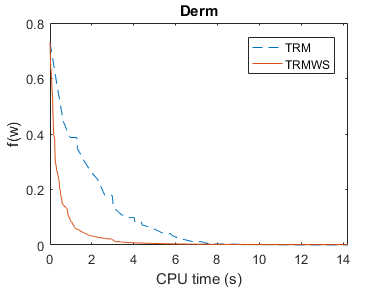
\includegraphics[width=\textwidth]{../../Desktop/Figures/Derm_TRMWS.png}
		\end{subfigure}
		\begin{subfigure}{.45\textwidth}
			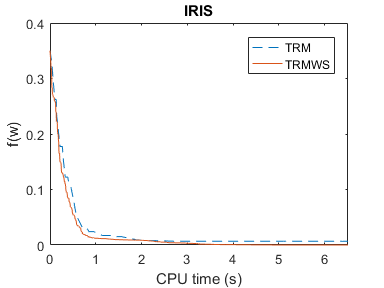
\includegraphics[width=\textwidth]{../../Desktop/Figures/IRIS_TRMWS.png}
		\end{subfigure}
		\begin{subfigure}{.45\textwidth}
			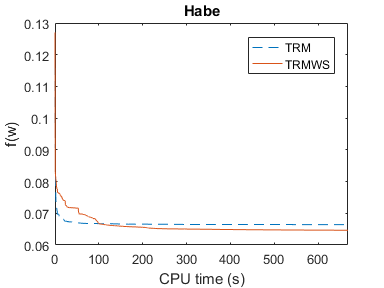
\includegraphics[width=\textwidth]{../../Desktop/Figures/Habe_TRMWS.png}
		\end{subfigure}
		\begin{subfigure}{.45\textwidth}
			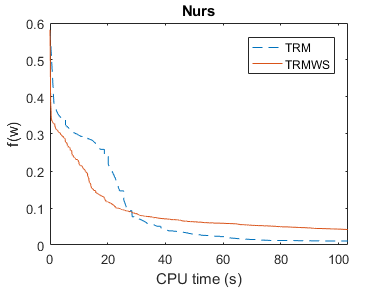
\includegraphics[width=\textwidth]{../../Desktop/Figures/Nurs_TRMWS.png}
		\end{subfigure}
		\begin{subfigure}{.45\textwidth}
			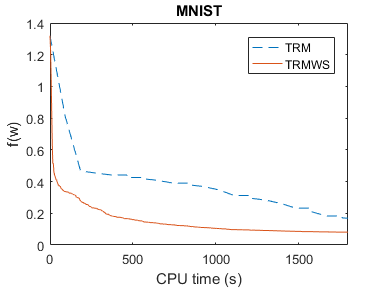
\includegraphics[width=\textwidth]{../../Desktop/Figures/MNIST_TRMWS.png}
		\end{subfigure}
		\caption{Running TRM vs TRMWS for training ff-ANNs on five datasets.}
		\label{figure:TRMWS}
	\end{figure}
	
	\begin{figure}
		\centering
		\begin{subfigure}{.45\textwidth}
			\includegraphics[width=\textwidth]{../../Desktop/figures/Derm_BTRMWS3.png}
		\end{subfigure}
		\begin{subfigure}{.45\textwidth}
			\includegraphics[width=\textwidth]{../../Desktop/figures/IRIS_BTRMWS3.png}
		\end{subfigure}
		\begin{subfigure}{.45\textwidth}
			\includegraphics[width=\textwidth]{../../Desktop/figures/Habe_BTRMWS3.png}
		\end{subfigure}
		\begin{subfigure}{.45\textwidth}
			\includegraphics[width=\textwidth]{../../Desktop/figures/Nurs_BTRMWS3.png}
		\end{subfigure}
		\begin{subfigure}{.45\textwidth}
			\includegraphics[width=\textwidth]{../../Desktop/figures/MNIST_BTRMWS3.png}
		\end{subfigure}
		\caption{Running BTRM vs BTRMWS for training ff-ANNs on five datasets.}
		\label{figure:BTRMWS}
	\end{figure}
	

	
	By looking at all of our results from applying weight subsampling together, the trend appears to be that the smaller the stochastic subset of training samples chosen at each iteration, the less effective adding weight subsampling will be to reduce TRRS. This result, though not entirely expected, is not surprising as every time a variation is made using a stochastic approach, the steps become less likely to lead to the solution of the overall problem. Once the sum of all approximated steps is no longer leading towards a minima for the full objective function, $f(\mathbf{w})$, they are no longer useful.
	
	\begin{figure}
		\centering
		\begin{subfigure}{.45\textwidth}
			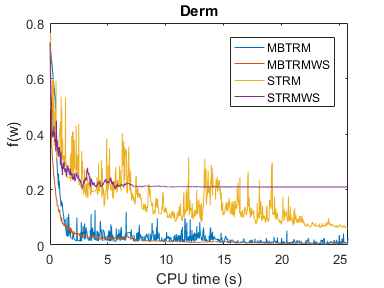
\includegraphics[width=\textwidth]{../../Desktop/Figures/Derm_SMBTRMWS2.png}
		\end{subfigure}
		\begin{subfigure}{.45\textwidth}
			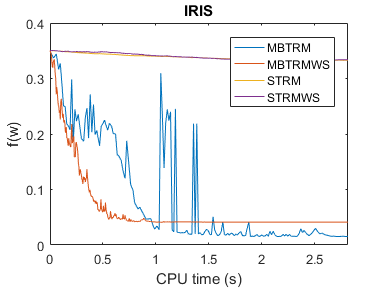
\includegraphics[width=\textwidth]{../../Desktop/Figures/IRIS_SMBTRMWS2.png}
		\end{subfigure}
		\begin{subfigure}{.45\textwidth}
			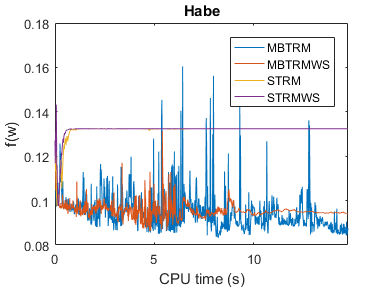
\includegraphics[width=\textwidth]{../../Desktop/Figures/Habe_SMBTRMWS2.png}
		\end{subfigure}
		\begin{subfigure}{.45\textwidth}
			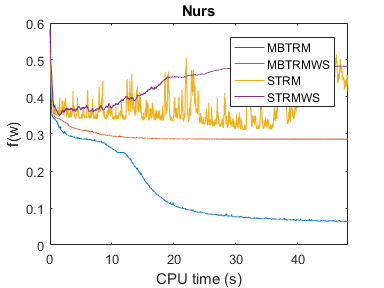
\includegraphics[width=\textwidth]{../../Desktop/Figures/Nurs_SMBTRMWS2.png}
		\end{subfigure}
		\begin{subfigure}{.45\textwidth}
			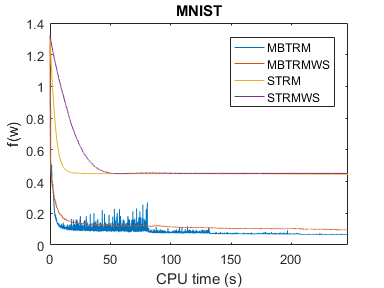
\includegraphics[width=\textwidth]{../../Desktop/Figures/MNIST_SMBTRMWS2.png}
		\end{subfigure}
		\caption{Test results for using stochastic TRM methods.}
		\label{figure:SMBTRMWS}
	\end{figure}
	
	\begin{table}[h] 
		\centering 
		\begin{tabular}{ |c||l|l||l|l|| } 
			\hline 
			\textbf{Dataset} & \textbf{MBTRM} & \textbf{MBTRMWS} & \textbf{STRM} & \textbf{STRMWS} \\ 
			\hline 
			\hline 
			Derm & $\mathbf{14.8783}$ &17.1257 & $\mathbf{22.0584}$ & -\\ 
			\hline 
			Habe & $\mathbf{8.1992}$ & - & $\mathbf{0.097114}$ &0.15717\\ 
			\hline 
			IRIS & $\mathbf{1.4322}$ & - & $\mathbf{14.1681}$ & -\\ 
			\hline 
			MNIST & $\mathbf{83.2774}$ & - & $\mathbf{17.2798}$ &46.9834\\ 
			\hline 
			Nurs & $\mathbf{55.4531}$ & - & $\mathbf{27.9826}$ & -\\ 
			\hline 
		\end{tabular} 
		\caption{TRRS results for $\Delta = 1\%$} \label{SMBTRMWS1} 
	\end{table}
	\begin{table}[h] 
		\centering 
		\begin{tabular}{ |c||l|l||l|l|| } 
			\hline 
			\textbf{Dataset} & \textbf{MBTRM} & \textbf{MBTRMWS} & \textbf{STRM} & \textbf{STRMWS} \\ 
			\hline 
			\hline 
			Derm & $\mathbf{1.455}$ &2.0583 & $\mathbf{10.3782}$ & -\\ 
			\hline 
			Habe & $\mathbf{2.0487}$ &4.4119 & $\mathbf{0.079468}$ &0.13661\\ 
			\hline 
			IRIS & $\mathbf{0.98844}$ & - & $\mathbf{2.4714}$ &3.2203\\ 
			\hline 
			MNIST & $\mathbf{6.4677}$ &31.6931 & $\mathbf{9.7466}$ &35.0008\\ 
			\hline 
			Nurs & $\mathbf{26.2484}$ & - & $\mathbf{9.0291}$ & -\\ 
			\hline 
		\end{tabular} 
		\caption{TRRS results for $\Delta = 5\%$} \label{SMBTRMWS5} 
	\end{table}
	\begin{table}[h] 
		\centering 
		\begin{tabular}{ |c||l|l||l|l|| } 
			\hline 
			\textbf{Dataset} & \textbf{MBTRM} & \textbf{MBTRMWS} & \textbf{STRM} & \textbf{STRMWS} \\ 
			\hline 
			\hline 
			Derm &1.2892 & $\mathbf{1.168}$ & $\mathbf{7.9418}$ & -\\ 
			\hline 
			Habe &0.96801 & $\mathbf{0.65215}$ & $\mathbf{0.061815}$ &0.11599\\ 
			\hline 
			IRIS &0.90709 & $\mathbf{0.54737}$ & 0 & 0 \\ 
			\hline 
			MNIST & $\mathbf{3.932}$ &7.9736 & $\mathbf{7.3748}$ &28.1962\\ 
			\hline 
			Nurs & $\mathbf{19.4037}$ & - & $\mathbf{0.50192}$ &0.9181\\ 
			\hline 
		\end{tabular} 
		\caption{TRRS results for $\Delta = 10\%$} \label{SMBTRMWS10} \end{table}
	
	
	
	\section{CPU Time Analysis}
	We study the profile of the CPU time expenditure for each Trust region derived method applied to each dataset. We exclude \textbf{TRMMBGD} which computes mainly stochastic mini-batch gradient steps and therefore cannot be compared directly. In order to make the comparison between remaining methods, we timed each component of an algorithm to determine if there are any outliers. It turns out that computing $\mathbf{H}_{k}$ for each iteration $k$, and $\mathbf{p}_{1}$ take the most time for all methods. This can be seen in Figures \ref{figure:p1_time} and \ref{figure:H_time}. For methods that require the computation of both $\mathbf{p}_{1}$ and $\mathbf{p}_{0}$, $\mathbf{p}_{0}$ always takes less than 12\% of the CPU time for an average step computation. If we sum together the time taken to compute $\mathbf{H}_{k}$, $\mathbf{p}_{1}$ and $\mathbf{p}_{0}$ (if $\mathbf{p}_{0}$ is applicable for that method) we find that these components contribute over 98\% of the CPU time. This gives us an explanation for why the second order methods, despite progressing more at each step, still produce longer TRRS values when compared to the gradient methods. It does show how Newton's method, equivalent to the instances where $\mathbf{p} = \mathbf{p}_{0}$ for \textbf{TRM}, is effective at computing a solution efficiently compared to computing the boundary step since the $\mathbf{p}_{0}$ computation takes much less time than the $\mathbf{p}_{1}$ computation as we can gather by comparing Figures \ref{figure:p1_time} and \ref{figure:p0_time}.
	\begin{figure}
		\centering
		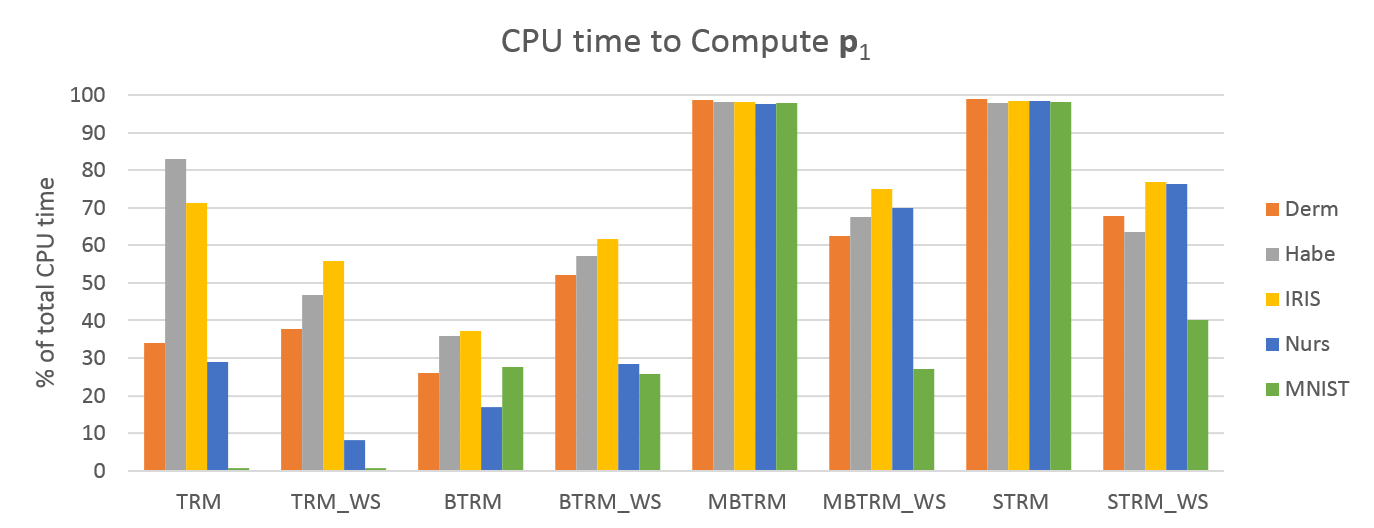
\includegraphics[width=\textwidth]{../../Desktop/Figures/CPU_time_p1_notitle.png}
		\caption{Percentage of time taken up by solving the Generalized Eigenvalue Problem (\ref{equation:M_def}) and computing $\mathbf{p}_{1}$ from the result at each step.}
		\label{figure:p1_time}
	\end{figure}
	\begin{figure}
		\centering
		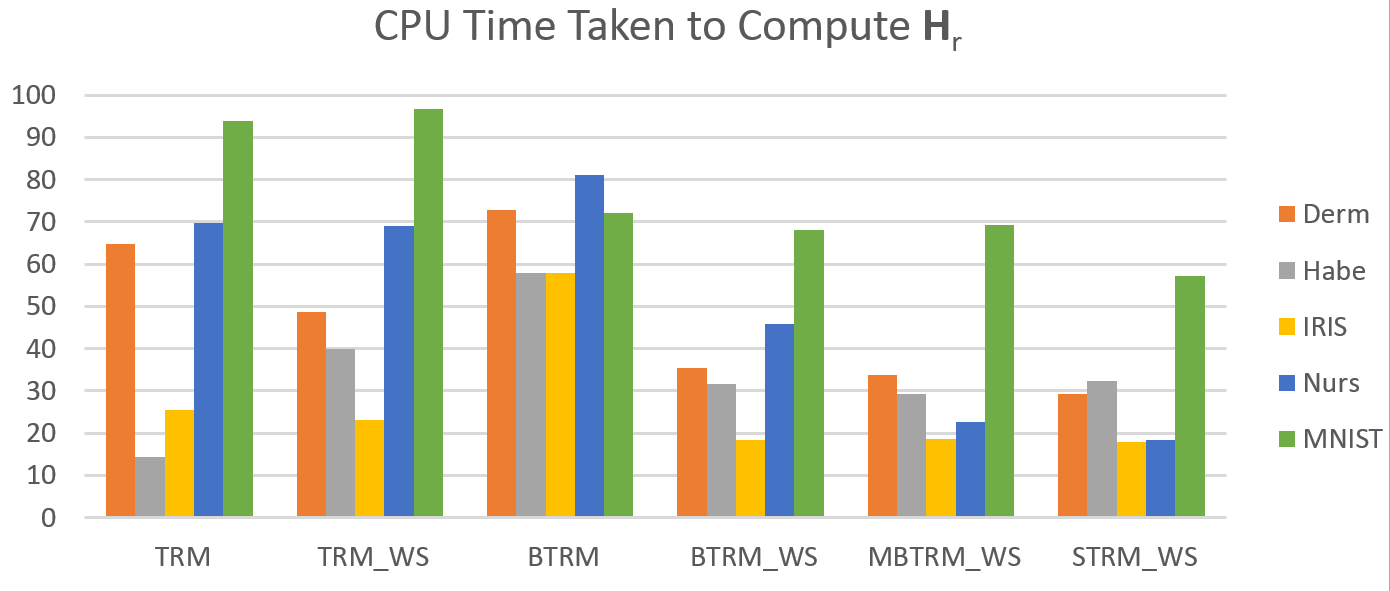
\includegraphics[width=\textwidth]{../../Desktop/Figures/CPU_time_H_notitle.png}
		\caption{Percentage of time taken for computing the Hessian matrix at each change in weight values $\mathbf{w}$. Recall that only five of our methods include the computation of the Hessian matrix. }
		\label{figure:H_time}
	\end{figure}
\begin{figure}
	\centering
	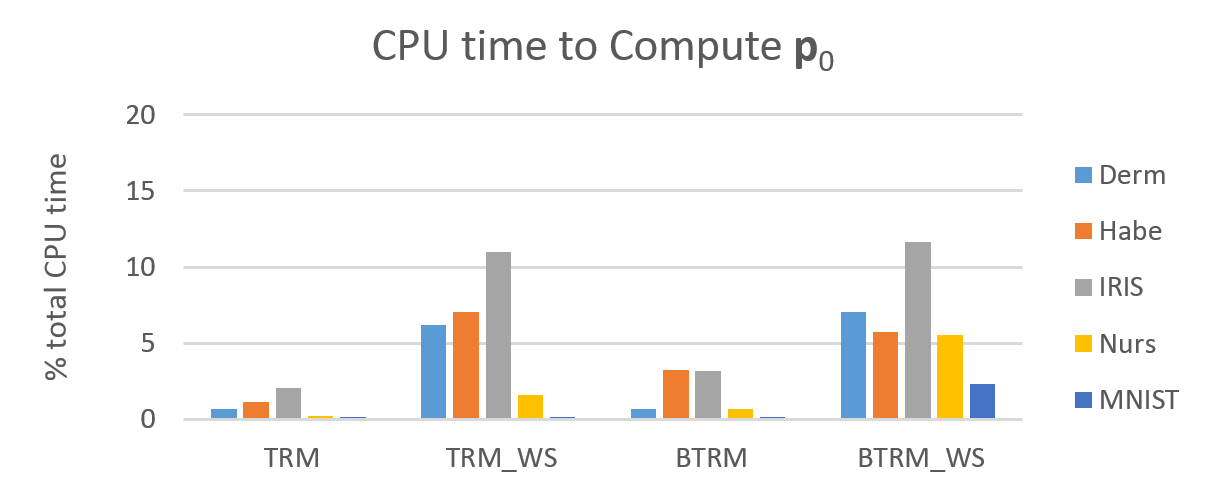
\includegraphics[width=\textwidth]{../../Desktop/Figures/CPU_time_p0_notitle.png}
	\caption{Percentage of time taken to solve for the $\mathbf{p}_{0}$, which is solving the linear equation (\ref{equation:p0}). Recall that those methods which use the ATRRS do not compute $\mathbf{p}_{0}$ (see Algorithm \ref{algorithm:assrs-simple}).}
	\label{figure:p0_time}
\end{figure}
	
	The $\mathbf{p}_{1}$ and $\mathbf{p}_{0}$ steps both involve iterative methods to determine their solution, namely ``eigs" in MATLAB and conjugate gradient, respectively. The algorithm is stopped when the relative residual is less than $10^{-3}$ for both ``eigs" and the conjugate gradient computation. Since convergence times depend on properties of the optimization problem that are out of our control, we decided to reduce these times by setting a very small limit on the number of iterations for each of the methods and accepting steps where the methods did not converge. We are changing the stopping criteria reaching a residual of $10^{-3}$ to reaching a max iteration number we refer to as \textbf{submaxiter}. In other words, the tests so far have been performed where convergence is achieved in order to solve the TRS at each step of the original problem. For the following methods, rather than waiting for convergence, we use the result achieved after \textbf{submaxiter} iterations regardless of it's accuracy to see how this performs. We compare these results to those where the method must converge to see if it speeds up the method. For most datasets the resulting behaviour is not notably different, this is likely because the datasets have a low number of parameters, $n$, and therefore may not need as many iterations to converge. On the other hand, we found a big difference in performance on the MNIST dataset, which is trained on the ff-ANN with the most parameters (1120), more than double the number of the next largest network. These results are displayed in Figure \ref{figure:mnist_maxiter}. When TRM with $\mathbf{p}_{1}$ and $\mathbf{p}_{0}$ convergence is compared with TRM run with a very low max iteration number for these two computations, and no convergence requirement, we see that TRM with convergence is more productive per epoch but much slower in terms of CPU time. Early stopping of $\mathbf{p}_{0}$ and $\mathbf{p}_{1}$ computations is shown here to produce less precise results in terms of step direction, but is significantly faster on problems with a large (in our case $>1000$) number of parameters. We compare with \textbf{SGD} to put the speed of the \textbf{submaxiter} \textbf{TRM} method in perspective. This comparison is shown in the bottom subfigure of Figure \ref{figure:mnist_maxiter}. We observe that despite seeing a speed up with \textbf{TRM}, the speed of objective function reduction still is much slower than that of \textbf{SGD}.
	
	
	\begin{figure}
		\centering
		\begin{subfigure}{.49\textwidth}
			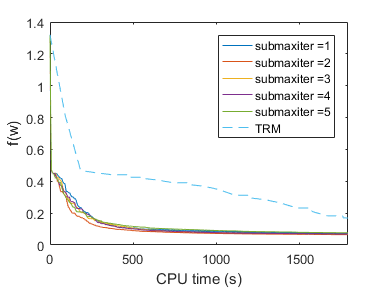
\includegraphics[width=\textwidth]{../../Desktop/figures/Submaxiter_noSGD.png}
		\end{subfigure}
		\begin{subfigure}{.49\textwidth}
			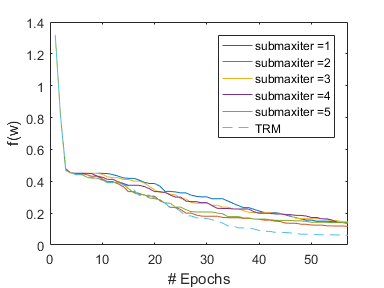
\includegraphics[width=\textwidth]{../../Desktop/figures/Submaxiter_epoch.png}
		\end{subfigure}
		\begin{subfigure}{.5\textwidth}
			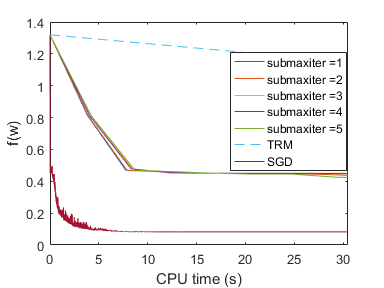
\includegraphics[width=\textwidth]{../../Desktop/figures/Submaxiter.png}
		\end{subfigure}
		\caption{Convergence of \textbf{TRM} with $\mathbf{p}_{0}$ and $\mathbf{p}_{1}$ using stopping criterion of residual magnitude less than $10^{-3}$ (dashed line) and stopping criterion of reaching the max iteration (\textbf{submaxiter}=1, 2, 3, 4, 5). (Upper Left) Convergence in terms of CPU time. (Upper Right) Convergence in terms of Epoch. (Bottom) Convergence in terms of CPU time with \textbf{SGD} for reference.}
		\label{figure:mnist_maxiter}
	\end{figure}
	
	\section{Robustness Test} 
	
	It is important to have some measure of robustness for an algorithm which is non-deterministic since outcomes may differ between experiment runs. We performed a robustness test on our algorithms by running them many times on the same small network and checking the accuracy of the solution. In order to perform this experiment we used a small network to compute the XOR output for two inputs on a two layer. This network can be trained quickly and also has a known saddle point, making it well suited to measure robustness.
	
	\subsection{The XOR Problem}
	
	The XOR problem that we use is specifically the two feature case of the XOR function. The total number of distinct values that a training sample can take is four, all of which are displayed in Table \ref{table:XOR}. In this test problem we use four training samples, one of each distinct value.
	
	\begin{table}[h] 
		\centering 
		\begin{tabular}{ |c|c||c| } 
			\hline 
			$\mathbf{x}_{1}$ & $\mathbf{x}_{2}$ & $y$\\ 
			\hline
			\hline
			0 & 0 & 0\\ 
			\hline 
			0 & 1 & 1\\ 
			\hline 
			1 & 0 & 1\\ 
			\hline 
			1 & 1 & 0\\ 
			\hline 
		\end{tabular} 
		\caption{The 2-feature XOR problem.} \label{table:XOR} \end{table}
	
	This is a very simple problem that contains classes which are not linearly separable. When trained on a two-layer network with two hidden nodes, the problem has a known saddle point, two local minima and a global mininum which are displayed in the Table \ref{table:XOR_point_type}.
	
	\begin{table}[h] 
		\centering 
		\begin{tabular}{ |c|c| } 
			\hline 
			$f(\mathbf{w})$ & \textbf{Point Type}\\ 
			\hline
			0.125 & saddle point\\  
			0.0625 & local minimum\\ 
			0.0833 & local minimum\\ 
			0 & global minimum\\ 
			\hline 
		\end{tabular} 
		\caption{First order critical point classification for the XOR problem when trained on a 2-layer ff-ANN with two hidden nodes.} \label{table:XOR_point_type} \end{table}
	
	Because of these known values, small size for fast training, and the known results of training a network on the XOR problem using various methods this is a well suited problem to test our methods for robustness by running each method many times and grouping the results. 
	
	\subsection{XOR Training Results}
	
	In order to see quantitatively how well all of these methods perform, we train a two layer ff-ANN to learn the XOR solution, and run it 1000 times on 100 initial weight settings in order to test robustness. We analyze our results by categorizing the final value of the objective function for each trial for each of our methods. We say a method has reached one of the four known points, $\mathbf{x}$, if the final objective function value achieved by the method is within $10^{-3}$ of $f(\mathbf{x})$. The value of these known points are displayed in Table \ref{table:XOR_point_type}. The results of this experiment are displayed in Figure \ref{figure:XOR}.
	
	 The hyperparameter procedure resulted in values for training example sampling: $b_{m}^{small} = b_{m}^{large} = m$, therefore \textbf{TRM} is equivalent to \textbf{BTRM} for this experiment so we do not show \textbf{BTRM} results. The mini-batch trust region methods, \textbf{MBTRM} and \textbf{MBTRMWS}, are still distinct from \textbf{TRM} and \textbf{TRMWS} respectively because of difference in $\gamma$ update method.  
	
	The results of the experiment are shown in Figure \ref{figure:XOR}. The first, most striking result, is the stochastic gradient descent, \textbf{SGD}, converges to the saddle point 100\% of the time. Its important to point out that this result could be dependent on the initial learning rate and learning rate schedule. It is still an interesting result and shows that with certain parameter choices, \textbf{SGD} may have difficulty converging to a minimizer. The promising takeaway for our methods is that \textbf{TRM}, \textbf{MBTRM}, \textbf{MBTRMWS}, and \textbf{TRMWS} all converge to a local minima for all 1000 trials. This shows that in this context, weight subsampling does not seem to affect the global convergence property of \textbf{TRM}, that is the method still converges to minima in all cases. 
	
	Another interesting result from this experiment is the improvement in performance between \textbf{MBGD} and \textbf{TRMMBGD}. We see that \textbf{TRMMBGD} increases the chances of at least resulting in a saddle point solution, compared to reaching no critical point for \textbf{MBGD}, and in some cases reaching the global minimum, compared to \textbf{MBGD} which most of the time does not reach a saddle point and never reaches a local or global minimum. When we look at all the results together that the percentage of times that a local minimum is reached can be predicted by the number of steps calculated using all 4 training examples of the XOR problem. That is, all methods that used $b_{m} = m$ at each step reached a local minimum 100\% of the time. \textbf{TRMMBGD}, which uses $b_{m} = 2$ most of the time and $b_{m} = m$ occasionally, reaches a local minimum occasionally. Finally those methods that never consider all training samples at the same step, $b_{m} < m$, never reach a local minimum. This is to be expected that stochastic subsampling of training samples is ineffective for the XOR problem since the classes for any set of three or fewer samples is linearly separable, therefore all four samples are required to represent the more complex XOR problem.
	
	\begin{figure}[h]
		\centering
		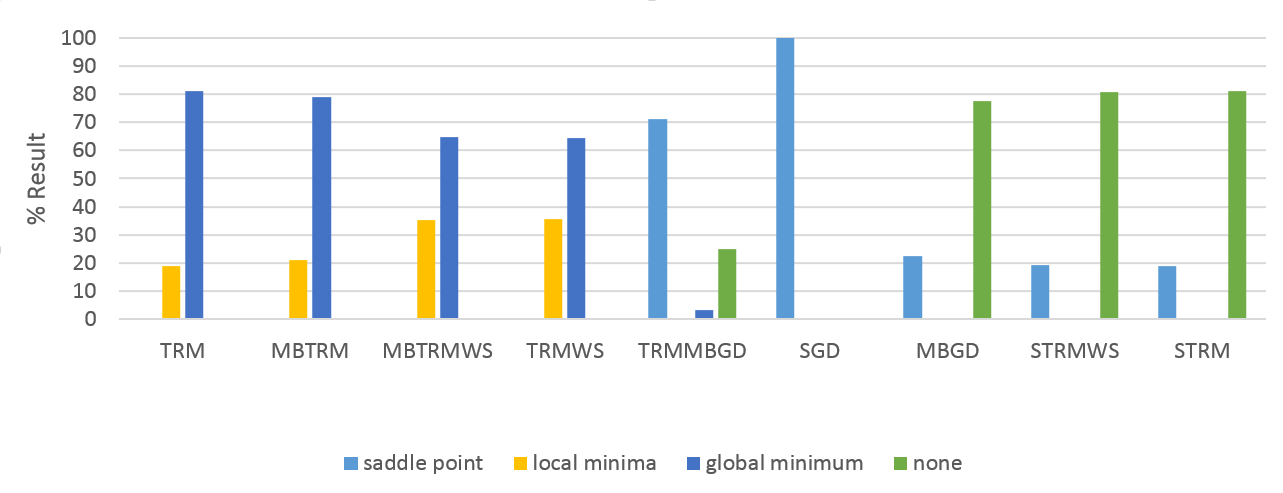
\includegraphics[width=\linewidth]{../../Desktop/figures/XOR_robustness2.PNG}
		\caption{Final points are recorded when the final objective function value is within a tolerance of $10^{-3}$ from one of the known points.}
		\label{figure:XOR}
	\end{figure}

	
	\begin{figure}[h]
		\centering
		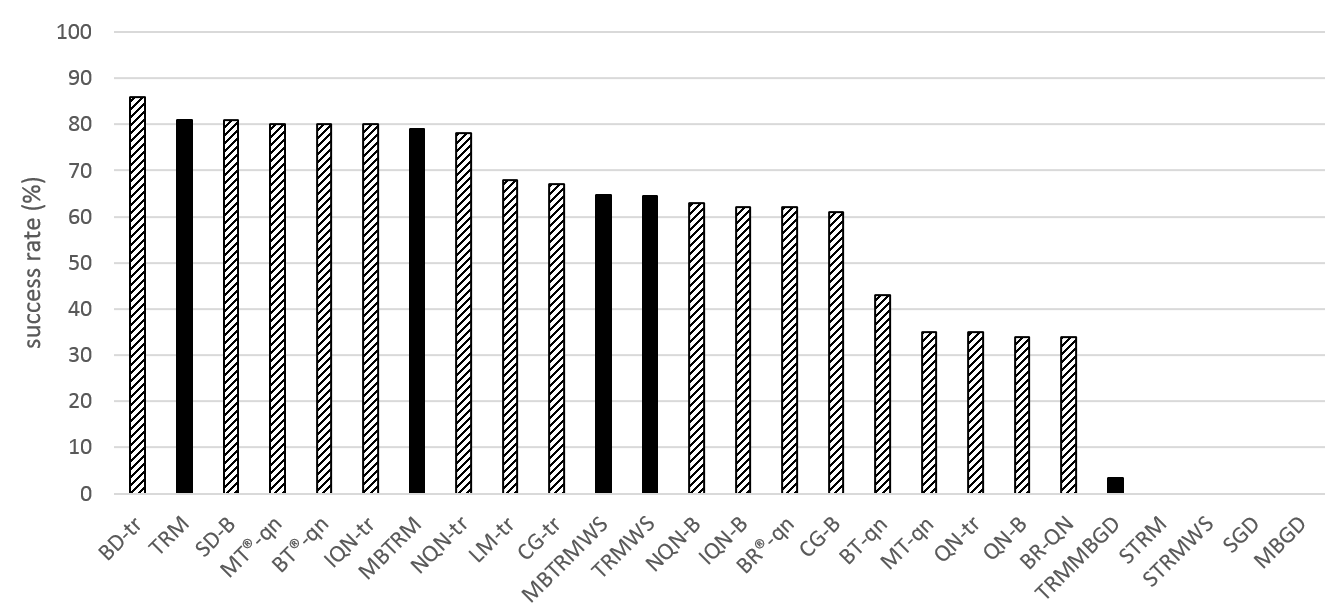
\includegraphics[width=\linewidth]{../../Desktop/figures/XOR_robustness_perceptron2.PNG}
		\caption{Percentage of runs which successfully converge to the global minimum of the XOR problem. The methods from our exploration are displayed as solid black and methods from \cite{Shepherd.1997} are coloured with a diagonal pattern.}
		\label{figure:XOR_comparison}
	\end{figure}
	Finally, we compare these results with those from other methods used to train the same two layer ff-ANN from \cite{Shepherd.1997}. This comparison is shown in Figure \ref{figure:XOR_comparison}. Methods with the suffix $-tr$ are methods that use the trust region model approach, those with $-B$ uses line minimization and those ending in $-qn$ are quasi-Newton methods. The full list of methods and their definitions are available on p. 134 of \cite{Shepherd.1997}.
	
	In Figure \ref{figure:XOR_comparison} we see that \textbf{TRM} manages to outperform all methods studied in \cite{Shepherd.1997}, with the exception of \textbf{BD-tr} which is the trust region model method with the bold driver method for adjusting the step size. The bold driver method simply increases the trust region radius when the previous step reduces the objective function, and decreases it otherwise. This is different from \textbf{TRM} which updates the trust region size based on the reliability of the second order model used within the bounds. This method therefore does not determine ``trust" of the second order model based on model accuracy but rather on reduction of the objective function, $f(\mathbf{w})$, a measure which does not take the model into consideration. In this thesis we decided to focus on methods derived from the more classical measure $\rho$, from (\ref{equation:rho}), which is based on model accuracy. 
	
	All of the methods from this thesis that use $b_{m} = m$ perform similarly to the trust region approaches tested in \cite{Shepherd.1997}, in terms of percentage of trials that reach the global minimum on the XOR problem. This simple problem does not show a very detailed comparison for training ff-ANNs in general but provides some context to show how these methods compare to a wide array of methods that have been studied in the context of training ff-ANNs. 
	
	\chapter{Conclusion}
	
	In this thesis, we studied a trust region approach, that uses the recent generalized eigenvalue method to solve the trust region subproblem (TRS), on training feedforward neural networks (ff-ANNs) by using the `Pearlmutter Trick' to compute the second order information. From this full method, we developed several variations of this learning algorithm that either estimate the TRS at an iteration, reduce the dimension of the TRS, or combine the trust region method with a stochastic gradient method. We used each of these methods to train networks on five datasets of different sizes and application domains. We analyzed these results to provide some insight as to the behaviour of these methods as well as a measure of CPU time taken to reach a reasonable solution, which provides an indicator of speed.
	
	Our results suggest that combining the trust region method presented in this thesis, along with mini-batch gradient descent, we can match or improve upon the speed of mini-batch gradient descent for all datasets tested. In terms of stochastic approximation approaches, we find that second order approximations using stochastic sampling were not beneficial for all datasets. However, results for using a large batch trust region method with the trust region size update showed that for most datasets a speed up in training results from large batch size sampling. We also find that with the largest dataset, MNIST, which requires the most parameters in a two-layer network, smaller batch stochastic sampling can be effective at speeding up the method. These results show promise for use on larger datasets.
	
	We find that weight subsampling at each iteration, which reduces the dimension of the TRS, can speed up the trust region method in some cases. It was particularly effective for the largest dataset tested, MNIST, on the largest network. This benefit however, was not seen, in a significant way, when used in combination with a stochastic sampling methods. Therefore, our results suggest that weight sampling can benefit trust region methods for problems with a larger number of test samples, $m$, and a larger number of parameters $n$. It should be considered, however, as an alternative to stochastic subsampling rather than a complementary method since we do not see the same benefits when used in tandem with a stochastic sampling method.
	
	The most useful result found in this investigation was the improvement or matching of solution and the time required for a reasonable solution (TRRS) for trust region used in tandem with mini-batch gradient descent as compared to mini-batch gradient descent on its own. This is a very promising result and indicates that other tandem methods may also be successful.
	
	 Despite some reduction of time required for a reasonable solution using stochastic subsampling and weight subsampling, these time reductions are still not large enough to improve upon the TRRS of a stochastic gradient descent method. Therefore, the benefit of a trust region method, without used in combination with a first order method, still lies purely in its ability to produce precise results and not in its speed.
	
	Overall, we have shed some light into the behaviour and performance changes of a specific approach to approximation of the trust region method used to train feedforward neural networks. We have also identified one method, the hybrid of the trust region method with mini-batch gradient descent, which does provide some improvements in speed and precision to mini-batch gradient descent.
	

	\section{Future Work}
	
	The most promising method that was tested in our numerical investigation was a hybrid method combining the complete trust region method with mini-batch gradient descent as was mentioned previously. We leave it as future work to determine what other methods can be improved for training neural networks when used in combination with the trust region method, or even a locally convergent method such as Newton's method.
	
	Another avenue of future work is to expand this survey to deeper networks and larger scale datasets. Since the trust region method has scaling difficulties, it is likely that the benefits of using approximate information become more obvious with larger datasets and a higher number of parameters in the network. This is something we see already with training on the MNIST dataset compared to the smaller datasets tested.
	
	The final interesting area that is left open for future exploration, is how to choose hyperparameters more effectively. This has been considered for training neural networks using more common approaches, but could be investigated further specifically for variations on trust region methods. 
	
	%ars The \appendix statement indicates the beginning of the appendices.
	\appendix
	
	% Add a title page before the appendices and a line in the Table of Contents
	\chapter*{APPENDICES}
	\addcontentsline{toc}{chapter}{APPENDICES}
	%======================================================================
	\chapter{Pearlmutter Trick for Computing Second Order Information}
	\label{appendix:pearlmutter}
	%----------------------------------------------------------------------
	
	In this section we discuss the use of the ``Pearlmutter Trick'' which can be used to exactly compute the matrix vector product of the Hessian, $\mathbf{H} \in \mathbb{R}^{n\times n}$, of an ff-ANN and any vector $\mathbf{v} \in \mathbb{R}^{n}$ \cite{Pearlmutter.1993}. In order to quickly compute the product $\mathbf{Hv}$, Pearlmutter developed a method based upon the ``R" operator which is a differential operator \cite{Pearlmutter.1993} defined as:
	
	\begin{equation}
	R_{\mathbf{v}}\{f(\mathbf{w})\} = \frac{\partial}{\partial r}f(\mathbf{w} + r\mathbf{v})\mid_{r=0} ,
	\end{equation}
	where $f(\mathbf{w})$ is the objective function we are looking to minimize, $\mathbf{w}$ is a vector of the parameters of the objective function (in the case of an ff-ANN these are the weights), and $\mathbf{v}$ can be interpreted as a direction vector to indicate in which direction to measure the derivative. For simplicity we will refer to $R_{\mathbf{v}}\{.\}$ simply as $R\{.\}$ Using this operator we are able to compute the $\mathbf{Hv}$ more easily since:
	
	\begin{equation}
	\mathbf{Hv} = \frac{\partial}{\partial r}\nabla{f}(\mathbf{w} + r\mathbf{v})\mid_{r=0} = R\{\nabla{f(\mathbf{w})}\}.
	\end{equation}
	
	Our goal is therefore to compute the result of using the R operator on the gradient of our objective function. Reaching this result requires a four pass method. The first two are the well known forward and back propagation passes for computing the gradient where we compute $f(\mathbf{w})$ using forward propagation, and $\nabla{f(\mathbf{w})}$ using back propagation. At this point we do a second forward/back propagation method at the end of which we are able to compute elements of $\mathbf{Hv}$.  The specific computations that make up these passes are described in $\S{3.1.1}$ and are referred to collectively as the ``Pearlmutter Trick".  
	
	\subsection{Forward and Back Propagations}
	\label{appendix:forandback}
	
	In this section we describe the forward and back propagation passes required to compute $R\{\nabla{f(\mathbf{w})}\}$ for an ff-ANN. Forward and back propagation methods are a way to reformat approaches to problems so that we can modularize layers in the ff-ANN setting and therefore implement general solutions that apply to all ff-ANNs rather than only a specific network. This is the concept for the use of forward and backpropagation to compute $\nabla{f(\mathbf{w})}$ and will be used as well to compute $R\{\nabla{f(\mathbf{w})}\}$.
	
	In this section there are some variables such as our weight variable $\mathbf{w}$ that are represented differently in the optimization setting than they are in the ff-ANN setting for ease of computations. Here is a list of equivalent values where on the left we have the representation used in optimization settings and on the right we have the representation most useful for training ff-ANNs:
	\begin{equation}
	\begin{split}
	&  n = \sum_{l=1}^{L}{n_{l}(n_{l-1}+1)} ,
	\\&    \mathbf{w} \leftrightarrow \{(\mathbf{W}_{1},\mathbf{b}_{1})\, (\mathbf{W}_{2},\mathbf{b}_{2}), ... , (\mathbf{W}_{L},\mathbf{b}_{L})\} ,
	\\&    \mathbf{v} \leftrightarrow \{(\mathbf{V}_{1},\mathbf{b}_{1}^{v})\, (\mathbf{V}_{2},\mathbf{b}_{2}^{v}), ... , (\mathbf{V}_{L},\mathbf{b}_{L}^{v})\} ,
	\label{equation:map}
	\end{split}    
	\end{equation}
	where $n_{l}$ represents the number of nodes computed at layer $l$, meaning that each layer computes a vector of size $n_{l}$ from a vector of size $n_{l-1}$. In the implementation of the TRM, $\mathbf{w}$ and $\mathbf{v}$ are concatenated vectorized matrices of their set on the right. The set on the right is the form of these weights for computations involved in the four passes of the ``Pearlmutter trick". A reverse mapping is also implemented. Let index $q$ be defined as:
	\begin{equation}
	q = \sum_{c=1}^{l-1}{n_{c}(n_{c-1}+1)} + (i-1)(n_{l-1}+1) + j,
	\label{equation:index}
	\end{equation}
	where $i$ and $j$ are the row and column indices respectively, for the matrix at layer $l$. The mapping by index is defined as:
	\begin{subequations}
		\begin{align}[left = {\mathbf{v}_{q} =(\mathbf{V}_{l},\mathbf{b}_{l}^{v})_{ij} = \empheqlbrace\,}]
		& (\mathbf{b}^{v}_{l})_{i}  \quad \text{if} \ j = (n_{l-1} + 1), \\
		& (\mathbf{V}_{l})_{ij} \quad  \text{otherwise}.
		\end{align}
		\label{equation:biasindex}
	\end{subequations}
	
	We note that we set $j = n_{l-1} + 1$ for bias values. Since we are computing $\mathbf{Hv}$ using backpropagation, the same mapping will apply here. That is to say, we want to compute all elements:
	\begin{equation}
	(\mathbf{Hv})_{q} =  R\{(\nabla f(\mathbf{w}))_{q}\} =  R\Big \{\frac{\partial{f(\mathbf{w})}}{\partial{\mathbf{w}_{q}}} \Big \} = R\Big \{\frac{\partial{f(\mathbf{w})}}{\partial{(\mathbf{W}_{l})_{ij}}} \Big \}, 
	\end{equation}
	where q corresponds to a weight value, otherwise $(\mathbf{Hv})_{q} =R\Big \{\frac{\partial{f(\mathbf{w})}}{\partial{(\mathbf{b}_{l}^{v})_{i}}} \Big \}$. In this section we show that in four passes, $R\{\frac{\partial{f(\mathbf{w})}}{\partial{(\mathbf{W}_{l})_{ij}}}\}$ and $R\Big \{\frac{\partial{f(\mathbf{w})}}{\partial{(\mathbf{b}_{l}^{v})_{i}}} \Big \}$ can be computed exactly for all $l$ and all possible associated values of $i$ and $j$. 
	
	The four propagation steps, or passes, that make up the ``Pearlmutter Trick" will be presented by what will be referred to as a respective \textbf{propagation equation} for each pass. How the \textbf{propagation equation} of an arbitrary pass is used to propagate throughout the layers of a network is shown in Algorithm \ref{algorithm:passes}. The values of some of the parameters used in Algorithm \ref{algorithm:passes} are dependent on whether the pass involves forward or backward propagation. Their values based on direction of propagation are presented in Table \ref{table:passes}.
	
	\begin{algorithm}
		\caption{Pseudocode of a Single Pass}\label{euclid}
		\begin{algorithmic}[1]
			\Procedure{Propagate example $k$}{}
			\State initialize $\mathbf{a}_{start}^{k}$
			\State $ l \gets start + incr$
			\While {$l \neq end$}
			\State $\mathbf{a}_{l}^{k} \gets \text{[\textbf{propagation equation}: unique for each pass]}(\mathbf{a}_{l-incr}^{k})$
			\State $l \gets l + incr$
			\EndWhile
			\EndProcedure
		\end{algorithmic}
		\label{algorithm:passes}
	\end{algorithm}
	In this Algorithm \ref{algorithm:passes}, $\mathbf{a}_{l}$ is the \textbf{propagating vector} for the pass at layer $l$ and the variables are based on the direction of the pass, defined in Table \ref{table:passes}.
	\begin{table}
		\begin{center}
			\begin{tabular}{ |c|c|c| } 
				\hline
				& forward & back \\
				\hline
				start & 0 & L \\ 
				end & L & 0 \\ 
				incr & +1 & -1 \\ 
				\hline
			\end{tabular}
			\caption{Values of parameters for Algorithm \ref{algorithm:passes} based on propagation direction.}
			\label{table:passes}
		\end{center}
	\end{table}
	$\mathbf{Note}$: This section assumes that all non-linear functions, $\sigma_{l}(.)$ map a single dependent variable from one independent variable for all layers $l$. This is not the case for all activation functions including the popular Softmax function for multi-class classification problems in machine learning and the difference in the form that the affected partial derivatives take is outlined at the end of $\S{3.6.1}$.
	
	\subsubsection{Forward Propagation I}
	
	In the first forward pass $\mathbf{a}^{k}_{l} = \mathbf{z}_{l}^{k}$, which is the propagating vector for step 5 of Algorithm \ref{algorithm:passes}.  $\mathbf{z}_{0}^{k}$ is initialized as the vector input for the training example $k$, $\mathbf{x}^{k}$, which is set prior to training. The propagation equation for this pass is given by:
	
	\begin{equation}
	(\mathbf{z}_{l}^{k})_{i} = \sigma_{l}((\mathbf{W}_{l})_{i}\mathbf{z}_{l-1}^{k} + (\mathbf{b}_{l})_{i}), 
	\label{equation:pass1_pe}
	\end{equation}
	where $\sigma_{l}(.)$ is the non-linear function at layer $l$, and $(\mathbf{W}_{l})_{i}$ is the $i^{th}$ row vector of the weight matrix at layer $l$. This allows us to compute the output of our final layer, $\mathbf{z}_{L}^{k}$, where $L$ is the number of layers. This forward propagation step is performed for each training example $k$ in our set of $m$ training examples. With this set of $m$ vectors $\mathbf{z}_{l}^{k}$, which depend on \textbf{w}, the objective function is now computed as:
	
	\begin{equation}
	f(\mathbf{w}) = \frac{1}{2m}\sum_{k=1}^{m}{(\mathbf{z}_{L}^{k} - \mathbf{y}^{k})^{T}(\mathbf{z}_{L}^{k} - \mathbf{y}^{k})},
	\end{equation}
	where $\mathbf{y}^k$ represents the vector of dependent variables of the $k^{th}$ training example, where training examples are presented as in (\ref{equation:training_example}), which is set at the time of training along with it's paired independent variable vector $\mathbf{x}^{k} = \mathbf{z}^{k}_{0}$.
	
	\subsubsection{Back Propagation I}
	
	In this pass the propagation vector, $\mathbf{a}^{k}_{l}$ from Algorithm \ref{algorithm:passes}, for each training example is the vector where the element at index $i$ is defined as  $\frac{\partial{f(\mathbf{w})}}{\partial{(\mathbf{z}^{k}_{l})_{i}}}$ and the vector is of length $n_{l}$. Initializing in this case involves defining this propagation vector at layer $L$ following our propagation procedure. Based on the objective function, the elements of this initial vector are:
	
	\begin{equation}
	\frac{\partial{f(\mathbf{w})}}{\partial{(\mathbf{z}^{k}_{L})_{i}}} = \frac{1}{m}((\mathbf{z}_{L}^{k})_{i} - \mathbf{y}^{k}_{i}).
	\label{equation:df_dzL0}
	\end{equation}
	This pass begins at the final layer, therefore $l = L$ for which $\frac{\partial{f(\mathbf{w})}}{\partial{(\mathbf{z}^{k}_{L})_{i}}}$ has already been computed using equation (\ref{equation:df_dzL0}) for $i=1,...,n_{L}$. The value of $\frac{\partial{f(\mathbf{w})}}{\partial{(\mathbf{z}^{k}_{L})_{i}}}$ are then each computed based on the previous layer. The propagation begins with the propagation equation used in Algorithm \ref{algorithm:passes} defined as:
	
	\begin{equation}
	\frac{\partial{f(\mathbf{w})}}{\partial{(\mathbf{z}_{l-1}^{k})_{i}}} = \sum_{j=0}^{n_{l}}{\frac{\partial{f(\mathbf{w})}}{\partial{(\mathbf{z}_{l}^{k})_{j}}}\sigma_{l}^{\prime}((\mathbf{W}_{l})_{j}\mathbf{z}_{l-1}^{k} + (\mathbf{b}_{l})_{i})(\mathbf{W}_{l})_{ij}}.
	\label{equation:pass2_pe}
	\end{equation}
	From this propagation procedure there is now sufficient information to compute the gradient defined as $\nabla{f(\mathbf{w})}$ where each element indexed by $q$ is defined as $\frac{\partial{f(\mathbf{w})}}{\partial{(\mathbf{W}_{l})_{ij}}}$ using the index mapping from (\ref{equation:index}). Each of these components is computed using:
	
	\begin{equation}
	\frac{\partial{f(\mathbf{w})}}{\partial{(\mathbf{W}_{l})_{ij}}} = \sum_{k=1}^{m}{\frac{\partial{f(\mathbf{w})}}{\partial{(\mathbf{z}_{l}^{k})_{i}}}\sigma_{l}^{\prime}((\mathbf{W}_{l})_{i}\mathbf{z}_{l-1}^{k}+ (\mathbf{b}_{l})_{i})(\mathbf{z}^{k}_{l-1})_{j}},
	\label{equation:grad_w}
	\end{equation}
	and
	\begin{equation}
	\frac{\partial{f(\mathbf{w})}}{\partial{(\mathbf{b}_{l})_{i}}} = \sum_{k=1}^{m}{\frac{\partial{f(\mathbf{w})}}{\partial{(\mathbf{z}_{l}^{k})_{i}}}\sigma_{l}^{\prime}((\mathbf{W}_{l})_{i}\mathbf{z}_{l-1}^{k}+ (\mathbf{b}_{l})_{i})},
	\label{equation:grad_b}
	\end{equation}
	where 
	\begin{equation}
	\sigma_{l}^{\prime}(x) = \frac{d\sigma_{l}(x)}{d x} \quad \forall x \in \mathbb{R}.
	\end{equation}
	For gradient methods this would be the propagation stopping point. The next two passes are required to compute Hessian related information and use values computed during these first two passes.
	
	
	\subsubsection{Forward Propagation II}
	
	In the second forward pass $\mathbf{a}_{l}^{k} = R\{\mathbf{z}_{l}^{k}\}$ for Algorithm \ref{algorithm:passes}. Since this is a forward pass, the vector that needs to be initialized is $R\{\mathbf{z_{0}}^{k}\}$. Because the R operator is a differential operator and $\mathbf{z}_{0}^{k}$ is the $k^{th}$ provided independent variable, $\mathbf{x}^k$, which is set prior to training and therefore treated as a constant:
	\begin{equation}
	R\{\mathbf{z_{0}}^{k}\} = \mathbf{0}.
	\end{equation}
	The propagation equation for Algorithm \ref{algorithm:passes} is determined by applying the ``R" operator to (\ref{equation:pass1_pe}). The ``R" operator follows all the rules of a differential operator so this is results in the following propagation equation:
	\begin{equation}
	\begin{split}
	R\{(\mathbf{z}_{l}^{k})_{i}\} & = R\{\sigma_{l}((\mathbf{W}_{l})_{i}\mathbf{z}_{l-1}^{k} + (\mathbf{b}_{l})_{i})\} \\ & = 
	\sigma_{l}^{\prime}((\mathbf{W}_{l})_{i}\mathbf{z}_{l-1}^{k} + (\mathbf{b}_{l})_{i})R\{(\mathbf{W}_{l})_{i}\mathbf{z}_{l-1}^{k} + (\mathbf{b}_{l})_{i}\} \\ & = 
	\sigma_{l}^{\prime}((\mathbf{W}_{l})_{i}\mathbf{z}^{k}_{l-1}+ (\mathbf{b}_{l})_{i})((\mathbf{W}_{l})_{i}R\{\mathbf{z_{l-1}^{k}}\} + (\mathbf{V}_{l})_{i}\mathbf{z}_{l-1}^{k} + (\mathbf{b}_{l}^{v})_{i}),
	\label{equation:pass3_pe}
	\end{split}
	\end{equation}
	since
	\begin{equation}
	R\{\mathbf{w}\} = \frac{\partial}{\partial r}(\mathbf{w} + r\mathbf{v})\mid_{r=0} = \mathbf{v},
	\end{equation}
	and
	\begin{equation}
	R\{\mathbf{w}\}_{q} = \mathbf{v}_{q},
	\label{equation:RwisV}
	\end{equation}
	which, when converted to matrix form using the mapping in (\ref{equation:index}), is equivalent to:
	\begin{equation}
	R\{(\mathbf{W}_{l})_{ij}\} = (\mathbf{V}_{l})_{ij},
	\label{equation:WtoV}
	\end{equation}
	and
	\begin{equation}
	R\{(\mathbf{b}_{l})_{i}\} = (\mathbf{b}^{v}_{l})_{i}.
	\label{equation:btobv}
	\end{equation}
	
	\subsubsection{Back Propagation II}
	
	In this final pass the propagation vector, $\mathbf{a}_{l}^{k}$, is set as the vector of size $n_{l}$ such that each element $i$ is defined by $R\{\frac{\partial{f(\mathbf{w})}}{\partial{(\mathbf{z}_{l}^{k})_{i}}}\}$. The ``R" operator is applied to (\ref{equation:df_dzL0}) for computing initial values $R\{\frac{\partial{f(\mathbf{w})}}{\partial{(\mathbf{z}_{L}^{k})_{i}}}\}$ which results in:
	\begin{equation}
	R\{\frac{\partial{f(\mathbf{w})}}{\partial{(\mathbf{z}_{L}^{k})_{i}}}\} = \frac{1}{m}R\{(\mathbf{z}_{L}^{k})_{i} - \mathbf{y}_{i}^{k}\} = \frac{1}{m}R\{(\mathbf{z}_{L}^{k})_{i}\},
	\end{equation}
	where $\mathbf{y}^{k}$ is the dependent variable vector for the $k^{th}$ training example which is set before optimization begins and therefore $R\{\mathbf{y}^{k}\} = \mathbf{0}$.
	
	For the propagation equation we can apply the ``R" operator on (\ref{equation:pass2_pe}). To simplify our final equation we can use this definition of an intermediate vector $\mathbf{h}_{l}^{k}$ where:
	\begin{equation}
	\mathbf{h}_{l}^{k} = \mathbf{W}_{l}\mathbf{z}_{l-1}^{k} + \mathbf{b}_{l},
	\end{equation}
	\begin{equation}
	\mathbf{z}_{l}^{k} = \sigma_{l}(\mathbf{h}_{l}^{k}).
	\end{equation}
	Using (\ref{equation:WtoV}) and (\ref{equation:btobv}) we can compute the result of using the ``R" operator on $\mathbf{h}_{l}^{k}$ as:
	\begin{equation}
	\begin{split}
	R\{\mathbf{h}_{l}^{k}\} & = R\{\mathbf{W}_{l}\}\mathbf{z}_{l-1}^{k} + \mathbf{W}_{l}R\{\mathbf{z}_{l-1}^{k}\} + R\{\mathbf{b}_{l}\}\\
	& = \mathbf{V}_{l}\mathbf{z}_{l-1}^{k} + \mathbf{W}_{l}R\{\mathbf{z}_{l-1}^{k}\} + \mathbf{b}_{l}^{v}.
	\label{equation:rh}
	\end{split}
	\end{equation}
	To further simplify our equation we define a second intermediate vector made up of the partial derivatives of $\mathbf{h}_{l}^{k}$ which are computed as:
	
	\begin{equation}
	\frac{\partial{f(\mathbf{w})}}{\partial{(\mathbf{h}_{l}^{k})_{i}}} = \frac{\partial{f(\mathbf{w})}}{\partial{(\mathbf{z}^{k}_{l})_{i}}}\frac{\partial{(\mathbf{z}^{k}_{l})_{i}}}{\partial{(\mathbf{h}^{k}_{l})_{i}}} = \frac{\partial{f(\mathbf{w})}}{\partial{(\mathbf{z}^{k}_{l})_{i}}}\sigma_{l}^{\prime}((\mathbf{h}_{l}^{k})_{i}), 
	\end{equation}
	and applying the ``R" operator we get:
	\begin{equation}
	\begin{split}
	R\{\frac{\partial{f(\mathbf{w})}}{\partial{(\mathbf{h}_{l}^{k})_{i}}}\} & = R\{\frac{\partial{f(\mathbf{w})}}{\partial{(\mathbf{z}^{k}_{l})_{i}}}\}\sigma_{l}^{\prime}((\mathbf{h}_{l}^{k})_{i}) + \frac{\partial{f(\mathbf{w})}}{\partial{(\mathbf{z}^{k}_{l})_{i}}}R\{\sigma_{l}^{\prime}((\mathbf{h}_{l}^{k})_{i}) \} \\
	& = R\{\frac{\partial{f(\mathbf{w})}}{\partial{(\mathbf{z}^{k}_{l})_{i}}}\}\sigma_{l}^{\prime}((\mathbf{h}_{l}^{k})_{i}) + \frac{\partial{f(\mathbf{w})}}{\partial{(\mathbf{z}^{k}_{l})_{i}}}\sigma_{l}^{\prime \prime}((\mathbf{h}_{l}^{k})_{i})R\{(\mathbf{h}_{l}^{k})_{i}\}.
	\label{equation:rdh}
	\end{split}
	\end{equation}
	With the above definitions to simplify the result, we apply ``R" to (\ref{equation:pass2_pe}) which results in the propagation equation:
	\begin{equation}
	\begin{split}
	R\{\frac{\partial{f(\mathbf{w})}}{\partial{(\mathbf{z}^{k}_{l-1})_{i}}}\} =
	& R\{\sum_{j=1}^{\mathbf{n_{l}}}{\frac{\partial{f(\mathbf{w})}}{\partial{(\mathbf{h}_{l}^{k})_{j}}}}(\mathbf{W}_{l})_{ij}\} \\
	=& \sum_{j=1}^{\mathbf{n_{l}}}{(R\{\frac{\partial{f(\mathbf{w})}}{\partial{(\mathbf{h}_{l}^{k})_{j}}}\}(\mathbf{W}_{l})_{ij} + \frac{\partial{f(\mathbf{w})}}{\partial{(\mathbf{h}_{l}^{k})_{j}}}R\{(\mathbf{W}_{l})_{ij}\})}\\
	=& \sum_{j=1}^{\mathbf{n_{l}}}{(R\{\frac{\partial{f(\mathbf{w})}}{\partial{(\mathbf{h}_{l}^{k})_{j}}}\}(\mathbf{W}_{l})_{ij} + \frac{\partial{f(\mathbf{w})}}{\partial{(\mathbf{h}_{l}^{k})_{j}}}(\mathbf{V}_{l})_{ij})}.
	\label{equation:pass4_pe}
	\end{split}
	\end{equation}
	This is all the information necessary to compute all values of $R\{\frac{\partial{f(\mathbf{w})}}{\partial{(\mathbf{W}_{l})_{ij}}}\}$ defined as:
	\begin{equation}
	\begin{split}
	R\{\frac{\partial{f(\mathbf{w})}}{\partial{(\mathbf{W}_{l})_{ij}}}\} = & \sum_{k=1}^{m}{R\{\frac{\partial{f(\mathbf{w})}}{\partial{(\mathbf{h}_{l}^{k})_{i}}}(\mathbf{z}_{l-1}^{k})_{j}\}} \\
	= & \sum_{k=1}^{m}{ R\{\frac{\partial{f(\mathbf{w})}}{\partial{(\mathbf{h}_{l}^{k})_{i}}}\}(\mathbf{z}_{l-1}^{k})_{j} + \frac{\partial{f(\mathbf{w})}}{\partial{(\mathbf{h}_{l}^{k})_{i}}}R\{(\mathbf{z}_{l-1}^{k})_{j}\}},
	\label{equation:hv_w}
	\end{split}
	\end{equation}
	and the equivalent for the bias values $(\mathbf{b}_{l})_{i}$:
	\begin{equation}
	R\{\frac{\partial{f(\mathbf{w})}}{\partial{(\mathbf{b}_{l})_{i}}}\} = \sum_{k=1}^{m}{ R\{\frac{\partial{f(\mathbf{w})}}{\partial{(\mathbf{h}_{l}^{k})_{i}}}\}}. 
	\label{equation:hv_b}
	\end{equation}
	Since $\mathbf{Hv} = R\{\nabla{f(\mathbf{w})}\}$  and we have computed every element of $R\{\nabla{f(\mathbf{w})}\}$ where
	
	\begin{subequations}
		\begin{align}[left = {\mathbf{Hv}_{q} =R\{\nabla{f(\mathbf{w}_{q})}\} =  \empheqlbrace\,}]
		& R\{\frac{\partial{f(\mathbf{w})}}{\partial{(\mathbf{b}_{l})_{i}}}\}  \quad \text{if} \ j = (n_{l-1} + 1), \\
		& R\{\frac{\partial{f(\mathbf{w})}}{\partial{(\mathbf{W}_{l})_{ij}}}\} \quad  \text{otherwise},
		\end{align}
		\label{equation:biasindex}
	\end{subequations}
	where the index mapping between $\mathbf{w}_{q}$ and $(\mathbf{W}_{l},\mathbf{b}_{l})_{ij}$ is defined by (\ref{equation:index}).
	
	\section{Complexity Analysis}
	
	In order to study speed up methods and to compare the TRM with gradient based methods we take this section to analyze the complexity of a single step of the TRM. 
	
	\subsection{Complexity Analysis of The Pearlmutter Trick for ff-ANNs}
	
	This section presents the complexity analysis of this method in order to quantify the scalability of the method and to take a step towards computing the complexity of the full TRS algorithm. Through the analysis of each of the four passes this method is shown to be bound by $O(mn)$ computations where $m$ is the number of training examples and $n$ is the number of parameters (weights). 
	
	\subsubsection{Forward Propagation I}
	
	During this first pass, the algorithm computes $\mathbf{z}_{l}^{k}$ using equation (\ref{equation:pass1_pe}) for every layer, $l=1,...,L$, and training example $k=1,...,m$. This requires computing $\mathbf{W}_{l}\mathbf{z}^{k}_{l-1} + \mathbf{b}_{l}$ which takes $n_{l}(n_{l-1} + 1)$ computations and then computing the non-linear function $\sigma_{l}(.)$ for all $n_{l}$ values of $\mathbf{W}_{l}\mathbf{z}^{k}_{l-1} + \mathbf{b}_{l}$, each of which takes constant time. Therefore the number of computations for the forward pass is:
	
	\begin{equation}
	\begin{split}
	T(n,m) = & \sum_{k=1}^{m}{\sum_{l=1}^{L}{n_{l}(n_{l-1} + 1) + cn_{l}}} \\
	= & m\sum_{l=1}^{L}{n_{l}(n_{l-1}+1) + cn_{l}},
	\end{split}
	\end{equation}
	using (\ref{equation:map}) we can simplify this to:
	\begin{align}
	\begin{split}
	T(n,m) & = m(n + c\sum_{l=1}^{L}{n_{l}}) \\
	& \leq mn(c + 1) \\
	& = O(mn)
	\end{split}
	\end{align}
	
	
	
	\subsubsection{Back Propagation I}
	
	During the second pass, the propagation equation (\ref{equation:pass2_pe}) computes $\sigma_{l}^{\prime}((\mathbf{W}_{l})_{j}\mathbf{z}_{l-1}^{k} + (\mathbf{b}_{l})_{i})$ which takes constant time determined by the non-linear function since the product $(\mathbf{W}_{l})_{j}\mathbf{z}_{l-1}^{k} + (\mathbf{b}_{l})_{i}$ has already been computed in the first forward pass. Finally we need then two constant time multiplications. This must happen for all $j \in n_{l}$ for a single derivative computation of which there are $n_{l-1}$ per layer. By this logic, we have:
	\begin{align}
	\begin{split}
	T(n,m) & =  \sum_{k=1}^{m}{\sum_{l=1}^{L}{\sum_{i=1}^{n_{l-1}}{{\sum_{j=1}^{n_{l}}{(c+2)}}}}} \\
	& = m\sum_{l=1}^{L}{(c+2)n_{l}n_{l-1}} \\
	& = (c+2)mn \\
	& = O(mn).
	\end{split}
	\end{align}
	The second set of values that need to be computed are the values of the gradient, $\frac{\partial{f(\mathbf{w})}}{\partial{(\mathbf{W}_{l})_{ij}}}$ and $\frac{\partial{f(\mathbf{w})}}{\partial{(\mathbf{b}_{l})_{i}}}$, which is done using (\ref{equation:grad_w}) and (\ref{equation:grad_b}) respectively. In this case $\sigma_{l}^{\prime}((\mathbf{W}_{l})_{j}\mathbf{z}_{l-1}^{k} + (\mathbf{b}_{l})_{i})$ has already been computed for (\ref{equation:pass2_pe}) so we have $m$ products of three scalars computed for each element value of $\mathbf{W}_{l} \in \mathbb{R}^{n_{l}n_{l-1}}$ at each layer and $m$ products of two scalars computed for each element value of $\mathbf{b}_{l} \in \mathbb{R}^{n_{l}}$ for each layer $l=1,...,n_{L}$. Therefore we count computations contributed from (3.11) to be:
	\begin{align}
	\begin{split}
	T(n,m) = & \sum_{l=1}^{L}{\sum_{i = 1}^{n_{l}}{{\sum_{k=1}^{m}{(\sum_{j=1}^{n_{l-1}}{2} + 1)}}}} \\
	< & 2m\sum_{l=1}^{L}{n_{l}(n_{l-1}+1)}\\
	= & 2mn \\
	= & O(mn),
	\end{split}
	\end{align}
	therefore, the number of operations required for this pass is bounded by $O(mn)$.
	
	\subsubsection{Forward Propagation II}
	
	During the third pass, which uses the propagation equation (\ref{equation:pass3_pe}), we note that the vector $\sigma_{l}^{\prime}((\mathbf{W}_{l})_{j}\mathbf{z}_{l-1}^{k} + (\mathbf{b}_{l})_{i})$ has already been computed during the previous pass for (\ref{equation:pass2_pe}). The two products $(\mathbf{W}_{l})_{i}R\{\mathbf{z_{l-1}^{k}}\}$ and  $(\mathbf{V}_{l})_{i}\mathbf{z}_{l-1}^{k}$ require $n_{l-1}$ computations each and then are added together so we can say that there are $cn_{l-1}$ computations total for a constant value $c$. The propagation equation, (\ref{equation:pass3_pe}), is computed for $i=1,...,n_{l}$, for $l=1,...,L$ for all $m$ training examples $k$. Therefore the runtime is:
	
	\begin{align}
	\begin{split}
	T(m,n) = & \sum_{k=1}^{m}{\sum_{l=1}^{L}{\sum_{i=1}^{n_l}{c(n_{l-1})}}} \\
	= & cm\sum_{l=1}^{L}{n_{l}n_{l-1}} \\
	= & cmn \\
	= & O(mn)
	\end{split}
	\end{align}
	
	\subsubsection{Back Propagation II}
	
	In (\ref{equation:rh}), there are $cn_{l}(n_{l-1}+1)$ computations to compute $ R\{\mathbf{h}_{l}^{k}\} $. Looking at (\ref{equation:rdh}), there are constant time operations for computing each value $(\mathbf{h}_{l}^{k})_{i}$, call this $c_{1}$. Therefore the total computations is:
	\begin{align}
	\begin{split}
	T(m,n) = & \sum_{k=1}^{m}{\sum_{l=1}^{L}{(\sum_{i=1}^{n_{l-1}}{\sum_{j=1}^{n_l}{c_{2}}} + cn_{l}(n_{l-1}+1) + \sum_{i=1}^{n_l}{c_{1}}})} \\
	= & \sum_{k=1}^{m}{\sum_{l=1}^{L}{((c + c_{2})n_{l}n_{l-1} + c_{1}n_{l})}} \\
	\leq & m\sum_{l=1}^{L}{((c + c_{1} + c_{2})n_{l}n_{l-1})} \\ 
	= & (c + c_{1} + c_{2})mn \\ 
	= & O(mn),
	\end{split} 
	\end{align}
	where $c_{2}$ is the amount of time to compute the right side of (3.21) within the sum.
	
	\subsubsection{Softmax vs Sigmoid}
	
	All analysis was done for non-linear functions, $\sigma_{l}(.)$, that produce a single dependent variable for a single independent varaible. That is, $\sigma_{l}(x) = y$ where $x, \ y \ \in \mathbb{R}$. Using a function such as softmax $\sigma_{l}(\mathbf{x}) = y$ where $\mathbf{x} \in \mathbb{R}^{w}$ and $y \in \mathbb{R}$ requires an extra bit of analysis. Recall that the number of output values in a layer computation is $n_{l}$ when we are iterating through multiple layers $l$. Here we look at what that difference is for completion of the algorithm. 
	
	$\mathbf{Sigmoid}$ (or any other function of one-to-one):\\
	The sigmoid function refers to:
	
	\begin{equation}
	\mathbf{z}_{i} = \sigma(\mathbf{h}_{i}) = \frac{1}{(1 + e^{-\mathbf{h}_{i}})}  ,
	\end{equation}
	where $\mathbf{z}_{i}, \mathbf{h}_{i} \in \mathbb{R}$ and the operation takes constant time. The first derivative of this function comes out to be:
	\begin{equation}
	\sigma^{\prime}(\mathbf{h}_{i}) = \sigma(\mathbf{h}_{i})(1-\sigma(\mathbf{h}_{i})),
	\end{equation}
	which also takes constant time and maps a single input to a single output. Finally, the second derivative is defined as:
	\begin{equation}
	\sigma^{\prime \prime}(\mathbf{h}_{i}) = \sigma^{\prime}(\mathbf{h}_{i})(1-2\sigma(\mathbf{h}_{i})),
	\end{equation}
	which can be computed in constant time as well. Therefore derivatives in terms of the objective function for our problem in terms of the inputs to the non-linear function are:
	\begin{equation}
	\frac{\partial{f(\mathbf{w})}}{\partial{\mathbf{h}_{i}}} = \frac{\partial{f(\mathbf{w})}}{\partial{\mathbf{z}_{i}}}\frac{\partial{\mathbf{z}_{i}}}{\partial{\mathbf{h}_{i}}} = \frac{\partial{f(\mathbf{w})}}{\partial{\mathbf{z}_{i}}}\sigma^{\prime}(\mathbf{h}_{i}),
	\end{equation}
	and:
	\begin{equation}
	\frac{\partial^{2}{f(\mathbf{w})}}{\partial{\mathbf{h}_{i}^{2}}} = \frac{\partial^{2}{f(\mathbf{w})}}{\partial{\mathbf{z}_{i}^{2}}}(\frac{\partial{\mathbf{z}_{i}}}{\partial{\mathbf{h}_{i}}})^{2} + \frac{\partial{f(\mathbf{w})}}{\partial{\mathbf{z}_{i}}}\frac{\partial^{2}{\mathbf{z}_{i}}}{\partial{\mathbf{h}_{i}^{2}}} = \frac{\partial^{2}{f(\mathbf{w})}}{\partial{\mathbf{z}_{i}^{2}}}\sigma^{\prime}(\mathbf{h}_{i}) + \frac{\partial{f(\mathbf{w})}}{\partial{\mathbf{z}_{i}}}\sigma^{\prime \prime}(\mathbf{h}_{i}).
	\end{equation}
	This confirms that applying the sigmoid function element-wise to the output vector of a layer takes $O(n_{l})$ complexity which is what we assumed in our analysis.
	
	$\mathbf{Softmax}$:
	The softmax function is defined as:
	\begin{equation}
	\sigma(\mathbf{h})_{i} = \frac{e^{\mathbf{h}_{i}}}{\sum_{j=1}^{n_{L}}{e^{\mathbf{h}_{j}}}},
	\end{equation}
	where the output, $\sigma(\mathbf{h})_{i}$ is a scalar and it requires all elements of the vector $\mathbf{h}$ to be computed. The runtime for computing a single output value appears to be $O(n_{L})$ based on the sum in the denominator, but can be made faster by computing the denominator once and then used for all values of $i=1,...,n_{L}$, therefore the runtime complexity bound for a single training example remains unchanged from sigmoid for forward propagation at $O(n_{l})$ where $l=L$ in the case of the final layer. 
	
	The partial derivatives $\frac{\partial{\mathbf{z}_{j}}}{\partial{\mathbf{h}_{i}}}$ for all $j=1,...,n_{l}$ are defined as follows:
	\begin{equation}
	\frac{\partial{\mathbf{z}_{j}}}{\partial{\mathbf{h}_{i}}} = -\mathbf{z}_{i}\mathbf{z}_{j} \quad \quad \forall i \neq j ,
	\label{equation:simplifieda}
	\end{equation}
	and
	\begin{equation}
	\frac{\partial{\mathbf{z}_{i}}}{\partial{\mathbf{h}_{i}}} = \mathbf{z}_{i}(1 - \mathbf{z}_{i}).
	\label{equation:simplifiedb}
	\end{equation}
	Finally, $\frac{\partial{f(\mathbf{w})}}{\partial{\mathbf{h}_{i}}}$ can be computed using the sum:
	\begin{equation}
	\frac{\partial{f(\mathbf{w})}}{\partial{\mathbf{h}_{i}}} = \sum_{j = 0}^{n-1}{\frac{\partial{f(\mathbf{w})}}{\partial{\mathbf{z}_{j}}}\frac{\partial{\mathbf{z}_{j}}}{\partial{\mathbf{h}_{i}}}} = \frac{\partial{f(\mathbf{w})}}{\partial{\mathbf{z}_{i}}}\mathbf{z}_{i} - (\mathbf{z}^{T}\frac{\partial{f(\mathbf{w})}}{\partial{\mathbf{z}}})\mathbf{z}_{i},
	\end{equation}
	which we computed using (\ref{equation:simplifieda}) as well as (\ref{equation:simplifiedb}), and $\frac{\partial{f(\mathbf{w})}}{\partial{\mathbf{z}}}$, is the vector such that:
	\begin{equation}
	(\frac{\partial{f(\mathbf{w})}}{\partial{\mathbf{z}}})_{i} = \frac{\partial{f(\mathbf{w})}}{\partial{\mathbf{z}_{i}}}
	\end{equation}
	which contains some $n_{l}$ computations where $\mathbf{h} \in \mathbb{R}^{n_{l}}$. However, the inner product $(\mathbf{z}^{T}\frac{\partial f(\mathbf{w})}{\partial{\mathbf{z}}})$ can be computed once in $O(n_{l})$ time and used to compute the output values for all $i \in n_{l}$. Therefore, the runtime complexity remains unchanged once again for back propagation I. 
	
	Finally we look at the second order derivative of the objective function in terms of the input to the non-linear function, $\mathbf{h}$. Firstly, the second derivatives of the softmax function are:
	
	\begin{equation}
	\frac{\partial^{2}{\mathbf{z}_{i}}}{\partial{\mathbf{h}_{i}}^{2}} = \mathbf{z}_{i}(1 - 2\mathbf{z}_{i}) + \mathbf{z}_{i}^2(2\mathbf{z}_{i} - 1) ,
	\end{equation}
	
	\begin{equation}
	\frac{\partial^{2}{\mathbf{z}_{j}}}{\partial{\mathbf{h}_{i}}^{2}} = \mathbf{z}_{j}\mathbf{z}_{i}(2\mathbf{z}_{i}-1) \quad \forall j \neq i.
	\end{equation}
	Using these results the second derivative, $\frac{\partial^{2}{f(\mathbf{w})}}{\partial{\mathbf{h}_{i}^{2}}}$, is defined as:
	
	\begin{equation}
	\begin{split}
	\frac{\partial^{2}{f(\mathbf{w})}}{\partial{\mathbf{h}_{i}^{2}}} = &\sum_{j = 1}^{n_{l}}({\frac{\partial^{2}{f(\mathbf{w})}}{\partial{\mathbf{z}_{j}}^{2}}(\frac{\partial{\mathbf{z}_{j}}}{\partial{\mathbf{h}_{i}}})^{2} +\frac{\partial{f(\mathbf{w})}}{\partial{\mathbf{z}_{j}}}\frac{\partial^{2}{\mathbf{z}_{j}}}{\partial{\mathbf{h}_{i}}^{2}}}) \\ = & \frac{\partial{f(\mathbf{w})}}{\partial{\mathbf{z}_{i}}}\mathbf{z}_{i}(1 - 2\mathbf{z}_{i})+\frac{\partial^{2}{f(\mathbf{w})}}{\partial{\mathbf{z}_{i}}^{2}}\mathbf{z}_{i}^{2}(1-2\mathbf{z}_{i})\\ &  + \sum_{j = 1}^{n_{l}}{\frac{\partial^{2}{f(\mathbf{w})}}{\partial{\mathbf{z}_{j}}^{2}}(\mathbf{z}_{i}\mathbf{z}_{j})^{2}} +\frac{\partial{f(\mathbf{w})}}{\partial{\mathbf{z}_{j}}}\mathbf{z}_{j}\mathbf{z}_{i}(2\mathbf{z}_{i}-1).
	\end{split}
	\end{equation}
	The summation in this equation takes $O(n_{l})$ to compute, but is the same for every value of $\frac{\partial^{2}{f(\mathbf{w})}}{\partial{\mathbf{h}_{i}^{2}}}$. Therefore, as before, the same runtime complexity can be achieved for both softmax and sigmoid non-linear functions. This shows that despite assuming there is a 1-to-1 mapping for the non-linear function used, the complexity analysis still applies to Softmax as the activation function used in the network.
	
	\chapter{Hyperparameters}
	\label{appendix:hyperparameters}
	
	As mentioned in Chapter 4, there are parameters that need to be chosen prior to training, we refer to these as hyperparameters to differentiate them from parameters or weights, which are tuned during training. The hyperparameters we consider before training are the weight subset size, $b_{w}$, the mini-batch size for trust region steps, $b_{m}^{small}$, the mini-batch size for gradient steps, $b_{m}^{GD}$, the large batch size $b_{m}^{large}$, the initial learning rate for stochastic gradient descent, $\gamma^{SGD}_{0}$, the initial learning rate for mini-batch gradient descent, $\gamma^{MBGD}_{0}$, the initial learning rate, or step size, for \textbf{STRM}, $\gamma^{STRM}_{0}$ and finally the initial learning rate, or step size, for \textbf{MBTRM}, $\gamma^{MBTRM}_{0}$. These hyperparameters are chosen using a line search type test protocol shown in Algorithm \ref{algorithm:hyperparameters}, where $f(\mathbf{w}_{i_{t}})$ is the objective function achieved at iteration $i_{t}$ where iteration $i_{t}$ is the smallest iteration count where the CPU time taken thus far is larger than $t$. Values of $incr$ and $p_{0}$ for each hyperparameter and dataset can be found in Appendix \ref{appendix:hyperparameter_values}, and the $\mathbf{Method}$ is chosen based on the parameter being tested using the mapping in Table \ref{table:hyperparameters}.
	
	\begin{algorithm}
		\caption{Hyperparameter Protocol}\label{algorithm:hyperparameters}
		\begin{algorithmic}[1]
			\Procedure{Find Suitable Hyperparameter}{}
			\State {Given: \textbf{Dataset}, $p_{0}$, $incr$, \textbf{Hyperparameter} }
			\State {\textbf{Method} $\gets$ from \textbf{Hyperparameter}, see Table \ref{table:hyperparameters}}
			\State $t$ $\gets$ CPU time for 10 iterations of $\mathbf{TRM}$
			\State $p \gets p_{0}$
			\State $error_{0} \gets$ $f(\mathbf{w}_{i_{t}})$ running \textbf{Method} on \textbf{Dataset} given $p$
			\State $i \gets 0$
			\State $error_{-1} = \infty$
			\While {$error_{i} < error_{i-1}$}
			\State $p \gets p + incr$
			\State $i = i + 1$
			\State $error_{i} \gets f(\mathbf{w}_{i_{t}})$ running \textbf{Method} on \textbf{Dataset} given $p$
			\EndWhile
			\Return{$p-incr$}
			\EndProcedure
		\end{algorithmic}
	\end{algorithm}
	
	\begin{table}[h]
		\centering
		\begin{tabular}{ |c|c| }  
			\hline
			\textbf{Hyperparameter} & \textbf{Method}\\
			\hline
			$b_{w}$ & \textbf{TRMWS} \\
			\hline
			$b_{m}^{GD}$ & \textbf{MBGD} \\
			\hline
			$b_{m}^{small}$ & \textbf{MBTRM} \\
			\hline
			$b_{m}^{large}$ & \textbf{BTRM} \\
			\hline
			$\gamma^{SGD}_{0}$ & \textbf{SGD} \\ 
			\hline
			$\gamma^{MBGD}_{0}$ & \textbf{MBGD} \\ 
			\hline
			$\gamma^{STRM}_{0}$ & \textbf{STRM} \\ 
			\hline
			$\gamma^{MBTRM}_{0}$ & \textbf{MBTRM} \\ 
			\hline
		\end{tabular}
		\caption{ The \textbf{Method} is the  algorithm used to test the \textbf{hyperparameter} in the same row. This mapping is used in Algorithm \ref{algorithm:hyperparameters}, row 3.}
		\label{table:hyperparameters}
		%\end{center}
	\end{table}
\chapter{Full Hessian vs Hessian Free}
\label{appendix:fhhf}
\begin{table}[h] 
	\centering 
	\begin{tabular}{ |c|l|l|l|l|l|l| } 
		\hline 
		\textbf{Dataset} & \textbf{IRIS} FH & \textbf{IRIS} HF & \textbf{Nurs} FH & \textbf{Nurs} HF & \textbf{Habe} FH & \textbf{Habe} HF \\ 
		\hline 
		TRM & $\mathbf{6.5095}$ &15.526 & $\mathbf{103.2252}$ &1393.098 & $\mathbf{562.1648}$ &1799.944\\
		\hline 
		BTRM &25.7475 & $\mathbf{22.2905}$ & $\mathbf{254.3873}$ &331.7311 &21.0777 & $\mathbf{20.9922}$\\ 
		\hline 
		MBTRM &1.6608 & $\mathbf{1.2765}$ &47.2323 & $\mathbf{24.9619}$ & $\mathbf{17.3623}$ &17.4178\\ 
		\hline 
		STRM &5.1491 & $\mathbf{3.7489}$ &35.5067 & $\mathbf{17.8883}$ &18.5672 & $\mathbf{17.6631}$\\ 
		\hline 
		TRMMBGD &0.62793 & $\mathbf{0.50674}$ &0.58953 & $\mathbf{0.51024}$ &0.31192 & $\mathbf{0.2718}$\\ 
		\hline 
		TRMWS & $\mathbf{6.539}$ &14.1964 & $\mathbf{67.2935}$ &306.8893 & $\mathbf{18.3271}$ &269.4662\\ 
		\hline 
		BTRMWS & $\mathbf{5.701}$ &11.1422 & $\mathbf{17.5241}$ &51.3723 & $\mathbf{11.4665}$ &21.4033\\ 
		\hline 
		MBTRMWS & $\mathbf{1.9442}$ &3.4353 & $\mathbf{7.2354}$ &13.1268 & $\mathbf{9.8883}$ &16.7996\\ 
		\hline 
		STRMWS & $\mathbf{4.6339}$ &8.0689 & $\mathbf{6.4347}$ &10.7207 & $\mathbf{10.3431}$ &18.0074\\ 
		\hline 
	\end{tabular} 
	\caption{Time taken to compute min(1000,max iterations) using the full H approach and the HF approach.} 
\end{table}


\begin{table}[h] 
	\centering 
	\begin{tabular}{ |c|l|l|l|l| } 
		\hline 
		\textbf{Dataset} & \textbf{MNIST} FH & \textbf{MNIST} HF & \textbf{Derm} FH & \textbf{Derm} HF \\ 
		\hline 
		TRM &3569.335 & $\mathbf{1731.513}$ &21.7445 & $\mathbf{14.5365}$\\ 
		\hline 
		BTRM &1798.383 & $\mathbf{235.8341}$ &151.3577 & $\mathbf{45.5098}$\\ 
		\hline 
		MBTRM &645.3847 & $\mathbf{46.7114}$ &109.1076 & $\mathbf{22.4816}$\\ 
		\hline 
		STRM &398.102 & $\mathbf{27.7807}$ &36.0154 & $\mathbf{8.4558}$\\ 
		\hline 
		TRMMBGD &1.224 & $\mathbf{1.1368}$ & $\mathbf{0.31795}$ &0.34063\\ 
		\hline 
		TRMWS & $\mathbf{203.0851}$ &1114.619 & $\mathbf{9.7145}$ &28.1894\\ 
		\hline 
		BTRMWS & $\mathbf{84.9487}$ &168.2657 & $\mathbf{13.1542}$ &25.5094\\ 
		\hline 
		MBTRMWS & $\mathbf{31.547}$ &32.5771 & $\mathbf{10.7201}$ &18.7424\\ 
		\hline 
		STRMWS & $\mathbf{20.5796}$ &21.3626 & $\mathbf{9.7782}$ &16.4827\\ 
		\hline 
	\end{tabular} 
	\caption{Time taken to compute min(1000,max iterations) iterations using the full H approach and the HF approach.} 
\end{table}
	
	\chapter{Hyperparameter Test Results}
	\label{appendix:hyperparameter_values}
	
	
	\begin{table}[h]
		\centering
		\begin{tabular}{ |c|c|c|c|c|c|c|c|c| }  
			\hline
			 & $\gamma_{0}$ & $\gamma_{0}$ & $\gamma_{0}$ & $\gamma_{0}$ &  &  &  &  \\
			\textbf{Dataset} & \textbf{SGD} & \textbf{MBGD} & \textbf{STRM} & \textbf{MBTRM} & $\mathbf{b_{w}}$ & $\mathbf{b}_{m}^{small}$ & $\mathbf{b}_{m}^{large}$ & $\mathbf{b}_{m}^{MBGD}$ \\
			
			\hline
			MNIST & 10 & 10 & 1.000000e-02 & 1 & 40 & 100 & 1000 & 100 \\
			\hline
			Derm & 1 & 10 & 1 & 1 & 15 & 20 & 75 & 10\\
			\hline
			IRIS & 1 & 1 & 0.01 & 1 & 5 & 15 & 50 & 5\\
			\hline
			Nurs & 1 & 10 & 0.1 & 0.1 & 5 & 60 & 1500 & 40\\
			\hline
			Habe & 0.01 & 0.1 & 0.1 & 0.1 & 15 & 10 & 75 & 5 \\ 
			\hline
			XOR & 0.1 & 0.1 & 0.001 & 1 & 4 & 4 & 4 & 2\\
			\hline
		\end{tabular}
		\caption{Final objective function achieved for training an ff-ANN on the set of datasets using SGD and using TRM.}
		\label{table:hyperparam}
		%\end{center}
	\end{table}
	
	%----------------------------------------------------------------------
	% END MATERIAL
	%----------------------------------------------------------------------
	
	% B I B L I O G R A P H Y
	% -----------------------
	
	% The following statement selects the style to use for references.  It controls the sort order of the entries in the bibliography and also the formatting for the in-text labels.
	\bibliographystyle{plain}
	% This specifies the location of the file containing the bibliographic information.  
	% It assumes you're using BibTeX (if not, why not?).
	\cleardoublepage % This is needed if the book class is used, to place the anchor in the correct page,
	% because the bibliography will start on its own page.
	% Use \clearpage instead if the document class uses the "oneside" argument
	\phantomsection  % With hyperref package, enables hyperlinking from the table of contents to bibliography             
	% The following statement causes the title "References" to be used for the bibliography section:
	\renewcommand*{\bibname}{References}
	
	% Add the References to the Table of Contents
	\addcontentsline{toc}{chapter}{\textbf{References}}
	
	\bibliography{uw-ethesis}
	% Tip 5: You can create multiple .bib files to organize your references. 
	% Just list them all in the \bibliogaphy command, separated by commas (no spaces).
	
	% The following statement causes the specified references to be added to the bibliography% even if they were not 
	% cited in the text. The asterisk is a wildcard that causes all entries in the bibliographic database to be included (optional).
	\nocite{*}
	
\end{document}